% Forcer la sortie PDF même si le compilateur Overleaf est réglé sur « LaTeX »
% (le moteur sous-jacent est pdfTeX ; sans ceci, on reste en mode DVI/dvips).
\pdfoutput=1

\documentclass[12pt,a4paper]{report}

\usepackage[T1]{fontenc}
\usepackage[utf8]{inputenc}
\usepackage[french]{babel}
\usepackage{lmodern}
\usepackage{microtype}
\usepackage{setspace}
\setstretch{1.25}

\usepackage{graphicx}
\DeclareGraphicsExtensions{.pdf,.png,.jpg,.jpeg}
\usepackage{geometry}
\geometry{margin=2.5cm}

% Charger xcolor avant tikz pour éviter le conflit d'options (tikz charge aussi xcolor).
\usepackage[table]{xcolor}
\usepackage{tikz}
\usetikzlibrary{arrows.meta, positioning, shapes.misc, shapes.geometric, shapes.multipart, calc, fit}

\usepackage{enumitem}
\setlist[itemize]{topsep=0.4em, itemsep=0.2em, leftmargin=1.5em}

\usepackage{fancyhdr}
\setlength{\headheight}{28pt}
\fancypagestyle{main}{
  \fancyhf{}
  \fancyhead[L]{\nouppercase{\leftmark}}
  \fancyfoot[C]{\thepage}
  \renewcommand{\headrulewidth}{0.4pt}
  \renewcommand{\footrulewidth}{0pt}
}

% Réduit les risques de lignes trop longues (overfull boxes)
\setlength{\emergencystretch}{2em}

\usepackage{booktabs}
\usepackage{longtable}
\usepackage{array}
\usepackage{tabularx}
\usepackage{float}
\newcolumntype{Y}{>{\raggedright\arraybackslash}X}
\newcolumntype{L}[1]{>{\raggedright\arraybackslash}p{#1}}
\newcommand{\tableheader}[1]{\textbf{\small #1}}
\newcommand{\tabarrow}{\ensuremath{\rightarrow}}

\usepackage{hyperref}
\hypersetup{
  colorlinks=true,
  linkcolor=black!70!blue,
  urlcolor=blue,
  citecolor=blue!70!black
}

% Citation auteur-année cliquable vers la bibliographie.
% Usage : \citer{davenport1998}{Davenport et Prusak (1998)}
% L'ancre correspondante dans la bibliographie est \label{ref:davenport1998}.
\newcommand{\citer}[2]{\hyperref[ref:#1]{#2}}

\usepackage{csquotes}
\usepackage{listings}
\lstset{
  basicstyle=\ttfamily\small,
  breaklines=true,
  frame=single,
  rulecolor=\color{black!20},
  backgroundcolor=\color{black!2},
  tabsize=2
}

% ---------------------------------------------------------------------------
% Métadonnées (à adapter si besoin)
% ---------------------------------------------------------------------------
\newcommand{\rapportTitre}{Vers une gestion documentaire intelligente : conception et réalisation d'une plateforme d'archivage numérique intégrant des mécanismes d'intelligence artificielle}
\newcommand{\auteurNom}{KOEVI Komi Pascal}
\newcommand{\typeDocument}{Mémoire pour le diplôme de}
\newcommand{\diplome}{Master professionnel en système d'information}
\newcommand{\formation}{Master Systèmes d’Information}
\newcommand{\universite}{LBS}
\newcommand{\nomEcole}{Lomé Business School}
\newcommand{\anneeAcademique}{2025--2026}
\newcommand{\nomMinistere}{Ministère de l'Efficacité du Service Public et de Transformation Numérique (MESPTN)}
\newcommand{\directeurNom}{M. KONAN Arnaud}
\newcommand{\directeurFonction}{Sr Machine Learning \& AI Engineer}
\newcommand{\structureAccueil}{Structure d’accueil : \textit{\nomMinistere}}
\newcommand{\tuteurStage}{Référent professionnel : \textit{M. Morlé KOUDEKA}}
\newcommand{\appNom}{ARIA}
\newcommand{\appDescription}{Archivage et Recherche par Intelligence Artificielle}

\title{\rapportTitre}
\author{\parbox{0.95\textwidth}{\centering
  \auteurNom\\
  \diplome\\
  \directeurNom\\
  \structureAccueil\\
  \tuteurStage
}}
\date{Avril 2026}

\begin{document}
% Page de garde (mise en page contrôlée, évite les débordements)
\begin{titlepage}
  \thispagestyle{empty}
  \centering
  \vspace*{1cm}
  {\Large \nomEcole\par}
  \vspace{1.5cm}

  {\large \typeDocument\par}
  \vspace{0.2cm}
  {\large \diplome}\par
  \vspace{2cm}

  {\LARGE \textbf{\rapportTitre}\par}
  \vspace{2.2cm}

  {\large Présenté par\par}
  \vspace{0.2cm}
  {\large \textbf{\auteurNom}\par}
  \vspace{1.5cm}

  {\large Directeur de Mémoire\par}
  \vspace{0.3cm}
  {\directeurNom\par}
  {\directeurFonction\par}
  \vspace{0.8cm}

  \vfill
  {Année universitaire 2023-2025\par}
\end{titlepage}

% Préliminaires (numérotation romaine)
% Ordre guide LBS : Remerciements → Dédicace → figures/tableaux → abréviations → résumé/abstract → TOC
\pagenumbering{roman}
\setcounter{page}{1}

\chapter*{Remerciements}
\addcontentsline{toc}{chapter}{Remerciements}
Je tiens tout d’abord à exprimer ma profonde gratitude au Ministère de l’Efficacité du Service Public et de la Transformation Numérique (MESPTN), au sein duquel j’exerce mes fonctions, pour le cadre professionnel, les ressources et la confiance qui m’ont permis de mener à bien ce projet et la rédaction de ce mémoire. Je remercie également l’ensemble de mes collègues pour leur disponibilité, leur collaboration et la qualité des échanges qui ont enrichi cette expérience, en particulier M. Songuimpale Koumbogle pour son soutien constant et ses précieux conseils tout au long du projet.

J’adresse mes sincères remerciements à M. Morlé KOUDEKA pour son encadrement, sa disponibilité et ses précieux conseils relatifs aux enjeux métiers de l’archivage numérique. Son expertise du domaine, sa vision stratégique ainsi que ses orientations ont largement contribué à la conception et à la réalisation de la solution proposée.

Je remercie également M. KONAN Arnaud, mon directeur de mémoire, pour la qualité de son accompagnement, la rigueur de ses observations et ses conseils éclairés sur les aspects techniques et méthodologiques liés à l’intelligence artificielle. Ses recommandations ont constitué un appui essentiel dans le développement du système et dans la rédaction de ce mémoire.

Ma reconnaissance s’adresse également à l’ensemble des collaborateurs du ministère qui, à travers leurs retours d’expérience, leurs échanges constructifs et leur disponibilité, ont contribué à affiner les besoins fonctionnels, à définir les règles de gestion documentaire et à orienter les choix de conception retenus pour cette plateforme intelligente d’archivage documentaire.

Je remercie Lomé Business School ainsi que l’ensemble du corps enseignant du Master Professionnel en Systèmes d’Information pour la qualité de la formation dispensée, les connaissances transmises et l’accompagnement méthodologique qui ont constitué un socle indispensable à la réalisation de ce travail.

Je tiens également à exprimer ma profonde gratitude à ma famille pour son soutien indéfectible, sa patience et ses encouragements tout au long de ce parcours. J’adresse une pensée particulière à mon frère Augustin pour ses relectures attentives, ses remarques pertinentes et les discussions enrichissantes qui ont nourri ma réflexion.

Enfin, je suis profondément reconnaissant envers toutes les personnes qui, de près ou de loin, ont contribué à la réussite de ce projet. Leur soutien, leurs conseils et leurs encouragements ont été une source constante de motivation et ont joué un rôle déterminant dans la concrétisation de ce mémoire et de la solution développée.

\clearpage
\chapter*{Dédicace}
\addcontentsline{toc}{chapter}{Dédicace}
\begin{flushright}
\vspace*{1cm}
\textbf{À ma famille,}\\[0.8em]
Pour son amour, son soutien indéfectible, ses sacrifices et ses encouragements constants tout au long de mon parcours académique et professionnel.\\[1.2em]
\textbf{À mes camarades, amis et collègues,}\\[0.8em]
Pour leur soutien moral, leurs échanges enrichissants et les moments de partage qui ont contribué à maintenir ma motivation et à enrichir ma réflexion.\\[1.2em]
\textbf{À toutes les personnes qui m’ont accompagné, soutenu et encouragé dans la poursuite de mes objectifs et de mes ambitions.}\\[1.2em]
Je dédie ce travail avec gratitude et reconnaissance.
\end{flushright}

\clearpage
\listoffigures
\clearpage
\listoftables
\clearpage

\chapter*{Liste des abréviations, sigles et acronymes}
\addcontentsline{toc}{chapter}{Liste des abréviations, sigles et acronymes}
\begin{description}[leftmargin=2.5cm, style=nextline]
  \item[ACL] \textit{Access Control List}
  \item[API] \textit{Application Programming Interface}
  \item[GED] Gestion électronique des documents
  \item[IA] Intelligence artificielle
  \item[IAM] \textit{Identity and Access Management}
  \item[LLM] \textit{Large Language Model}
  \item[MFA] \textit{Multi-Factor Authentication}
  \item[OAIS] \textit{Open Archival Information System}
  \item[OCR] \textit{Optical Character Recognition}
  \item[RBAC] \textit{Role-Based Access Control}
  \item[RAG] \textit{Retrieval-Augmented Generation}
  \item[RRF] \textit{Reciprocal Rank Fusion}
  \item[SSO] \textit{Single Sign-On}
  \item[TAL] Traitement automatique du langage
  \item[TLS] \textit{Transport Layer Security}
\end{description}

\clearpage
\chapter*{Résumé}
\addcontentsline{toc}{chapter}{Résumé}
Un document scanné n’est pas encore une archive. Dans les administrations publiques, la gestion documentaire repose encore largement sur des supports papier et sur des pratiques de classement hétérogènes, rendant l’accès à l’information difficile, lent et peu fiable. Au \nomMinistere{}, des milliers de documents anciens, dont certains remontent à 1906, devaient être numérisés dans un délai contraint, tout en restant exploitables au quotidien.

L’enjeu principal consistait ainsi à transformer un volume important de documents numérisés en archives structurées, correctement nommées, classées et facilement retrouvables.

Ce rapport présente la conception et la réalisation d’un système d’archivage numérique déployé en environnement \textit{on-premise}. La solution proposée permet l’ingestion automatique des documents depuis plusieurs scanners via des dossiers partagés, puis déclenche une chaîne de traitement basée sur des techniques d’intelligence artificielle : reconnaissance optique de caractères (OCR), extraction d’informations, structuration des données et génération de métadonnées. Ces traitements permettent de proposer automatiquement un renommage et un classement conformes aux règles définies par le ministère, tout en laissant à l’utilisateur la possibilité de valider ou corriger les résultats via une interface web dédiée.

L’architecture du système repose sur une approche microservices, garantissant la scalabilité, la résilience et la modularité de la solution. En complément, un assistant conversationnel permet d’interroger le contenu documentaire en langage naturel. Les réponses sont générées à partir d’un contexte extrait des documents archivés, selon une approche de recherche sémantique couplée à la génération augmentée par récupération (\textit{RAG}), améliorant significativement l’accès à l’information.

Ainsi, la solution mise en place permet d’industrialiser le processus d’archivage numérique en réduisant les tâches manuelles, en améliorant la qualité et la cohérence du classement, et en garantissant la traçabilité des opérations. Elle répond également aux exigences de sécurité et de souveraineté grâce à un déploiement en environnement interne.

\noindent\textbf{Mots-clés :} archivage numérique ; intelligence artificielle ; RAG ; OCR ; administration publique.

\chapter*{Abstract}
\addcontentsline{toc}{chapter}{Abstract}
A scanned document is not yet an archive. In public administrations, document management still relies heavily on paper-based workflows and heterogeneous filing practices, making access to information difficult, slow, and unreliable. At the \nomMinistere{}, thousands of legacy documents, some dating back to 1906, had to be digitized within a constrained timeframe while remaining usable on a daily basis.

The main challenge was therefore to transform a large volume of digitized documents into structured archives that are properly named, consistently classified, and easy to retrieve.

This report presents the design and implementation of an on-premise digital archiving system. The proposed solution enables automatic ingestion of documents from multiple scanners through shared network folders, then triggers an AI-driven processing pipeline: optical character recognition (OCR), information extraction, data structuring, and metadata generation. These capabilities support automated suggestions for file naming and classification according to predefined rules, while allowing users to validate or correct the results through a dedicated web interface.

The system architecture follows a microservices approach to ensure scalability, resilience, and modularity. In addition, a conversational assistant allows users to query the document corpus in natural language. Answers are generated from relevant document context using semantic search combined with retrieval-augmented generation (RAG), significantly improving access to information.

\noindent\textbf{Keywords:} digital archiving; artificial intelligence; RAG; OCR; public administration.

\clearpage
\tableofcontents
\clearpage

% Corps du document (numérotation arabe + en-têtes/pieds de page)
\pagenumbering{arabic}
\pagestyle{main}

\chapter*{Introduction}
\addcontentsline{toc}{chapter}{Introduction}
L'information est aujourd'hui reconnue comme l'une des ressources les plus stratégiques des organisations. Dans les administrations publiques, elle constitue le fondement de l'action administrative, assure la continuité du service public, garantit la transparence des décisions et participe à la préservation de la mémoire institutionnelle. Chaque courrier, rapport, arrêté, contrat, note de service ou document réglementaire représente une trace des activités de l'administration et contribue à la constitution d'un patrimoine documentaire dont la valeur dépasse largement son usage immédiat. Correctement conservé, organisé, sécurisé et exploité, ce patrimoine devient un levier essentiel de gouvernance, de pilotage et d'aide à la décision.

Cependant, une part importante de ce patrimoine documentaire demeure encore conservée sous format papier dans de nombreuses administrations publiques. Accumulés pendant plusieurs années, voire plusieurs décennies, ces fonds documentaires représentent une richesse informationnelle considérable, mais leur exploitation reste limitée par les contraintes liées aux supports physiques : difficultés de classement, risques de détérioration, temps nécessaire à la recherche d'informations et absence de mécanismes permettant une exploitation rapide et intelligente des contenus. Ainsi, la préservation et la valorisation de ces archives nécessitent aujourd'hui une approche dépassant la simple conservation physique des documents.

L'accélération de la transformation numérique a profondément modifié la manière dont le patrimoine documentaire est produit, traité et conservé. La dématérialisation progressive des procédures administratives, la généralisation des services numériques et l'évolution des outils collaboratifs ont entraîné une croissance continue du volume documentaire produit par les organisations. Parallèlement, les administrations doivent désormais gérer une diversité importante de ressources : documents papier historiques nécessitant une numérisation, fichiers bureautiques, courriers électroniques, images numérisées, feuilles de calcul, présentations, contenus audiovisuels, archives compressées et autres formats numériques hétérogènes. Cette coexistence entre documents physiques à transformer et documents numériques natifs donne naissance à un patrimoine documentaire multimodal dont la gestion constitue un défi majeur pour les systèmes d'information.

Face à cette évolution, les plateformes de Gestion Électronique des Documents (GED) se sont progressivement imposées comme des outils essentiels de modernisation des organisations. Elles permettent de centraliser les documents, d'en assurer le stockage, l'indexation, le partage et la conservation tout au long de leur cycle de vie. Toutefois, ces solutions interviennent généralement après la numérisation des documents et restent encore largement dépendantes d'opérations manuelles réalisées par les utilisateurs pour l'indexation, la description des contenus, la classification ou l'organisation des documents. Lorsque les volumes documentaires deviennent importants, notamment lors de projets de numérisation massive d'archives papier, ces opérations deviennent longues, coûteuses et sources d'erreurs, limitant ainsi la capacité des organisations à exploiter efficacement leur patrimoine documentaire.

La problématique ne réside donc plus uniquement dans la conversion des documents papier en fichiers numériques, mais dans la capacité des organisations à transformer ces nouveaux contenus numériques en une ressource informationnelle structurée et exploitable. La numérisation constitue une première étape indispensable, mais elle ne garantit pas à elle seule la valorisation des archives. Les documents obtenus doivent être identifiés, classifiés, enrichis par des métadonnées pertinentes, organisés selon des règles documentaires cohérentes et rendus facilement accessibles aux utilisateurs concernés. La gestion documentaire évolue ainsi d'une logique de simple stockage vers une logique de valorisation intelligente de la connaissance contenue dans les archives.

Les progrès récents de l'intelligence artificielle offrent des perspectives particulièrement prometteuses pour répondre à ces nouveaux défis. Les avancées en reconnaissance optique de caractères (OCR), en vision par ordinateur, en traitement automatique du langage naturel, en apprentissage profond et, plus récemment, en grands modèles de langage (\textit{Large Language Models}) permettent aujourd'hui d'automatiser des tâches auparavant réalisées exclusivement par l'humain. Ces technologies rendent possible l'extraction automatique d'informations depuis des documents numérisés, la génération de métadonnées, la classification intelligente, la reconnaissance d'entités, le renommage automatique des fichiers, la détection de similarités documentaires ainsi que la recherche sémantique dans des corpus volumineux. Les approches fondées sur le \textit{Retrieval-Augmented Generation} (RAG) ouvrent également la voie à de nouvelles formes d'interaction avec les archives, en permettant aux utilisateurs d'interroger leur patrimoine documentaire en langage naturel.

Toutefois, l'intégration de l'intelligence artificielle dans les systèmes documentaires ne peut se limiter à une simple évolution technologique. Dans le domaine des archives publiques, où l'authenticité, l'intégrité, la confidentialité, la disponibilité et la traçabilité des documents constituent des exigences fondamentales, l'intelligence artificielle doit être conçue comme un outil d'assistance au service des archivistes et des gestionnaires de l'information. Elle doit permettre de réduire les tâches répétitives et d'améliorer l'efficacité des traitements documentaires, tout en respectant les principes archivistiques et les règles de gouvernance documentaire.

Au Togo, la modernisation de l'administration publique s'inscrit dans une dynamique de transformation numérique visant à améliorer l'efficacité des services publics, à renforcer la transparence administrative et à promouvoir une meilleure gouvernance de l'information. Dans ce cadre, plusieurs institutions ont engagé des initiatives visant à numériser leurs archives physiques afin de préserver le patrimoine documentaire national et d'en faciliter l'accès. Toutefois, ces projets de numérisation font apparaître de nouveaux défis liés au traitement de grandes quantités de documents numérisés : identification du contenu, classement, indexation, organisation logique des archives et recherche efficace de l'information. La transformation d'un document papier en fichier numérique ne constitue donc qu'une étape intermédiaire ; elle doit être accompagnée de mécanismes intelligents permettant d'exploiter pleinement la valeur informationnelle des archives.

C'est dans ce contexte que s'inscrit le présent mémoire intitulé \textbf{« \rapportTitre{} »}. Ce travail trouve son origine dans un projet de transformation numérique d'un fonds documentaire composé de plusieurs milliers de documents papier issus d'une administration publique togolaise. L'objectif initial était de préserver ces archives physiques par leur numérisation. Cependant, cette opération a rapidement mis en évidence une problématique majeure : une fois les documents convertis en fichiers numériques, leur organisation représentait toujours un défi important.

En effet, le traitement manuel des documents numérisés nécessitait de nombreuses interventions humaines pour l'identification des informations pertinentes, l'extraction des métadonnées, la détermination des catégories documentaires, le renommage des fichiers, l'identification des expéditeurs et leur classement dans une structure archivistique cohérente. Face au volume important des documents traités, ces opérations devenaient particulièrement longues, complexes et susceptibles d'introduire des incohérences dans l'organisation finale des archives.

Afin de répondre à ces défis, ce mémoire propose \textbf{\appNom{}} (\textit{\appDescription{}}), une plateforme intelligente de gestion documentaire multimodale conçue pour accompagner la transformation des archives papier en archives numériques intelligemment organisées. La plateforme intervient dans l'ensemble du cycle de transformation documentaire, depuis l'exploitation des documents issus de la numérisation jusqu'à leur classification, leur organisation et leur recherche avancée. Elle prend également en charge les documents nativement numériques afin de répondre aux besoins actuels des administrations.

\appNom{} repose sur une architecture orientée services intégrant un stockage objet compatible S3 permettant la gestion de ressources documentaires hétérogènes. Les mécanismes d'intelligence artificielle intégrés automatisent notamment l'extraction de métadonnées, la classification documentaire, le renommage intelligent, la reconnaissance d'entités, la recherche sémantique et l'assistance aux utilisateurs, tout en garantissant les exigences de sécurité, de traçabilité et de gouvernance propres aux environnements administratifs.

Cette situation conduit à la problématique suivante :

\textbf{Comment concevoir une plateforme intelligente de gestion documentaire multimodale capable d'accompagner la transformation des archives papier vers des archives numériques intelligemment organisées, tout en exploitant les capacités de l'intelligence artificielle afin d'améliorer la classification, la recherche et la valorisation du patrimoine documentaire de l'administration publique togolaise ?}

Pour répondre à cette problématique, ce mémoire poursuit comme objectif principal la conception et la réalisation d'une plateforme intelligente de gestion documentaire multimodale intégrant des techniques d'intelligence artificielle afin d'automatiser le traitement documentaire et d'améliorer la valorisation des archives administratives. Plus spécifiquement, il s'agit d'analyser les besoins liés à la transformation des archives papier, de concevoir une architecture adaptée à un environnement documentaire multimodal, de développer une plateforme fonctionnelle intégrant des mécanismes d'intelligence artificielle et d'évaluer les apports de cette approche dans un contexte réel d'utilisation.

Le présent mémoire est organisé en plusieurs parties. Le premier chapitre présente les fondements de la gestion documentaire intelligente : notions d'information, de document et de patrimoine documentaire, principes d'archivage numérique, évolution des systèmes de GED, multimodalité et technologies d'intelligence artificielle mobilisées. Le deuxième chapitre situe l'étude dans le contexte de la transformation numérique de l'administration publique togolaise et précise la problématique liée au traitement des archives. La partie suivante analyse le fonctionnement documentaire existant au \nomMinistere{} et spécifie les besoins de la plateforme, avant de décrire la conception et la réalisation de \appNom{}, puis l'évaluation, l'exploitation et le bilan de la démarche.

\chapter*{Présentation de Lomé Business School}
\addcontentsline{toc}{chapter}{Présentation de Lomé Business School}
Lomé Business School (LBS) est un établissement d’enseignement supérieur situé à Lomé (Togo), engagé dans la formation de cadres et de professionnels capables de répondre aux besoins du tissu économique et institutionnel. L’école propose des parcours de Licence et de Master dans des domaines liés au management, à la finance, au marketing et aux systèmes d’information, avec une orientation professionnalisante fondée sur l’articulation entre enseignements théoriques et mises en situation pratiques.

Dans le cadre du Master professionnel en Systèmes d’Information, la formation vise à doter les étudiants de compétences en conception, développement, déploiement et gouvernance des systèmes d’information. Elle combine des apports académiques (méthodologie de recherche, architecture logicielle, bases de données, sécurité) et une immersion professionnelle via le stage de fin de cycle. Le mémoire constitue l’aboutissement de ce parcours : il doit articuler une problématique scientifique ou technique, une revue des connaissances existantes et une expérience de terrain, tout en respectant les normes de rédaction et de validation définies par l’établissement.

Le présent travail s’inscrit pleinement dans cette logique. Il a été réalisé sous la direction de M. KONAN Arnaud, dans le cadre d’une mission menée au \nomMinistere{}, et répond aux exigences du diplôme de Master professionnel en systèmes d’information de Lomé Business School. Il illustre la volonté de l’école de former des profils capables de concevoir des solutions numériques sobres, sécurisées et adaptées aux contraintes des organisations publiques.

\part{Fondements théoriques et contexte de l'étude}
\chapter{Fondements de la gestion documentaire intelligente}
La gestion documentaire constitue un enjeu essentiel pour les organisations qui doivent produire, conserver, retrouver et exploiter un volume croissant d'informations. L'évolution des pratiques administratives et la transformation numérique ont progressivement fait évoluer les méthodes de gestion des documents, depuis les approches principalement fondées sur le support papier vers des environnements numériques capables de traiter des ressources documentaires hétérogènes.

Cette évolution ne concerne pas uniquement le stockage des documents. Elle touche également leur identification, leur description, leur classement, leur conservation et leur exploitation. Les systèmes de Gestion Électronique des Documents (GED) ont ainsi apporté des mécanismes permettant de structurer et de sécuriser les ressources documentaires. Les progrès de l'intelligence artificielle ouvrent aujourd'hui une nouvelle étape en permettant d'automatiser certaines opérations d'analyse et de traitement documentaire.

Ce chapitre présente les principaux concepts nécessaires à la compréhension de cette évolution. Il aborde successivement la relation entre information, document et patrimoine documentaire, les principes de la gestion documentaire et de l'archivage numérique, l'évolution des systèmes de GED vers des plateformes plus intelligentes, la gestion des documents multimodaux et les principales technologies d'intelligence artificielle appliquées au traitement documentaire.

\section{De l'information au patrimoine documentaire}
La compréhension de la gestion documentaire repose d'abord sur la distinction entre l'information, le document et le patrimoine documentaire. Ces trois notions sont liées : l'information constitue le contenu à exploiter, le document permet de la fixer et de la transmettre, tandis que l'ensemble des documents produits et conservés par une organisation forme progressivement son patrimoine documentaire.

\subsection{L'information : une ressource stratégique}
L'information peut être considérée comme une donnée interprétée et replacée dans un contexte lui donnant une signification. Elle permet notamment de comprendre une situation, de réduire l'incertitude et de soutenir la prise de décision.

Dans une organisation, l'information intervient dans les activités opérationnelles, la coordination des acteurs, le suivi des décisions et la conservation de la mémoire institutionnelle. Sa valeur dépend donc non seulement de son contenu, mais également de sa disponibilité, de sa fiabilité et de sa capacité à être retrouvée au moment nécessaire. Cette perspective rejoint les travaux de \citer{davenport1998}{Davenport et Prusak (1998)}, qui insistent sur le rôle stratégique de l'information et de la connaissance dans le fonctionnement des organisations, ainsi que sur la nécessité de les gérer et de les exploiter efficacement.

La transformation numérique a considérablement augmenté les volumes d'informations produits et échangés. Cette évolution renforce l'intérêt de mécanismes permettant de les structurer, de les sécuriser et de les exploiter efficacement. Le document constitue l'un des principaux moyens utilisés pour fixer et conserver cette information.

\subsection{Le document : support de l'information}
Un document est un support sur lequel une information est fixée afin d'être conservée, transmise ou exploitée. Il peut être physique ou numérique et prendre des formes variées : texte, image, tableau, présentation, courrier électronique, fichier audio ou vidéo.

Conformément à la norme \citer{iso15489}{ISO~15489-1:2016}, les documents d'activité doivent être gérés indépendamment de leur structure ou de leur forme, dès lors qu'ils constituent une preuve ou une trace des activités de l'organisation. Cette approche permet de ne pas limiter le concept de document aux seuls fichiers bureautiques ou aux formats PDF.

Dans les environnements numériques, la facilité de production et de duplication des documents entraîne une augmentation importante des volumes documentaires. La gestion de ces ressources nécessite alors de disposer d'informations permettant de les identifier, de les contextualiser et de les retrouver.

La valeur d'un document ne dépend donc pas uniquement de son contenu. Elle dépend également de son contexte, de son origine, de son authenticité, de son intégrité et des informations qui permettent de le retrouver et de l'exploiter, conformément aux principes rappelés par la norme \citer{iso15489}{ISO~15489-1:2016}.

\subsection{Le patrimoine documentaire : mémoire des organisations}
Les documents produits ou reçus dans le cadre des activités d'une organisation constituent progressivement un patrimoine documentaire. Certains sont conservés en raison de leur valeur administrative, juridique, historique ou informationnelle.

\citer{unesco2015}{L'UNESCO (2015)} considère le patrimoine documentaire comme un héritage devant être préservé, protégé et rendu accessible, y compris sous forme numérique. Ce patrimoine permet notamment de conserver les traces des activités réalisées, de justifier certaines décisions et de maintenir une continuité documentaire malgré l'évolution des organisations. Sa valeur dépend toutefois de la capacité de l'organisation à maintenir les documents accessibles, compréhensibles et exploitables dans le temps.

La gestion du patrimoine documentaire implique ainsi des règles et des dispositifs permettant d'assurer son organisation, sa conservation et son accès. Ces principes conduisent naturellement aux notions de gestion documentaire et d'archivage.

\section{Gestion documentaire et archivage numérique}
La gestion documentaire regroupe les pratiques et les mécanismes permettant de maîtriser les documents produits ou reçus par une organisation tout au long de leur cycle de vie. L'archivage constitue une dimension particulière de cette gestion, centrée sur la conservation des documents présentant une valeur durable.

\subsection{Les principes de la gestion documentaire}
La gestion documentaire vise notamment à organiser les documents, contrôler leur accès, faciliter leur recherche et garantir leur conservation selon les règles définies par l'organisation.

La norme \citer{iso15489}{ISO~15489-1:2016} met l'accent sur la maîtrise du cycle de vie des documents d'activité et sur les propriétés qui en garantissent la valeur dans le temps : authenticité, fiabilité, intégrité et exploitabilité. Elle précise également les principes relatifs à la création, à la capture et à la gestion des documents, ainsi qu'aux politiques, responsabilités et systèmes documentaires associés.

Ces principes nécessitent des règles de classement, des droits d'accès et des mécanismes de traçabilité adaptés. Les métadonnées y jouent un rôle central : la norme \citer{iso23081}{ISO~23081-1:2017} en définit les principes de gestion afin d'assurer l'identification, le contexte et l'exploitabilité des documents d'activité.

\subsection{De la capture numérique à l'archivage numérique}
La transition d'un document physique vers un environnement numérique commence par sa capture. Celle-ci consiste à produire une représentation numérique du document, notamment au moyen d'un dispositif de numérisation. Dans la logique de la norme \citer{iso15489}{ISO~15489-1:2016}, la capture constitue une étape de gestion documentaire, et non une fin en soi.

Numérisation et archivage numérique ne se confondent donc pas. Le fichier obtenu doit encore pouvoir être identifié, décrit, classé, stocké et retrouvé. L'archivage numérique ajoute des exigences de conservation et d'accès dans le temps. Le modèle de référence OAIS (\citer{iso14721}{ISO~14721:2025}) définit un système d'archivage comme un ensemble combinant matériel, logiciel, informations, politiques et processus, mis en œuvre afin de préserver l'information et de la rendre disponible à une communauté désignée.

Les bonnes pratiques de préservation numérique rappellent par ailleurs que l'évolution technologique peut rendre des contenus inutilisables si leur environnement de lecture devient obsolète (\citer{dpc}{Digital Preservation Coalition (s.d.)}). La valeur d'un document numérique dépend ainsi de son organisation, de ses métadonnées et des dispositifs qui en assurent la conservation.

\subsection{Les exigences de l'archivage numérique}
L'archivage numérique doit permettre de maintenir les documents accessibles et exploitables sur la durée tout en préservant leurs caractéristiques essentielles. Ces exigences rejoignent les propriétés rappelées par la norme \citer{iso15489}{ISO~15489-1:2016} et se déclinent notamment ainsi :
\begin{itemize}
  \item l'authenticité, permettant d'établir qu'un document est bien celui qu'il prétend être ;
  \item l'intégrité, garantissant que son contenu n'a pas été altéré de manière non autorisée ;
  \item la traçabilité, permettant de suivre les opérations réalisées sur le document ;
  \item la disponibilité, assurant son accès aux personnes autorisées ;
  \item l'exploitabilité, permettant de retrouver et d'interpréter l'information dans le temps.
\end{itemize}

Le modèle OAIS (\citer{iso14721}{ISO~14721:2025}) complète cette perspective en précisant les responsabilités liées à la conservation et à l'accessibilité à long terme, tandis que \citer{dpc}{Digital Preservation Coalition (s.d.)} met en évidence les risques technologiques et organisationnels associés à l'obsolescence des formats et des environnements de lecture. L'archivage numérique ne peut donc être réduit à une simple fonction de stockage : il suppose une organisation cohérente des documents, de leurs métadonnées et des règles qui encadrent leur conservation.

\subsection{Les limites des approches traditionnelles à grande échelle}
Lorsque les volumes documentaires restent limités, les opérations de description, de classement et d'indexation peuvent être réalisées manuellement. Leur maintien devient plus difficile lorsque le nombre de documents augmente et que les ressources deviennent plus hétérogènes.

Le traitement manuel présente alors plusieurs limites : temps important consacré à l'analyse, dépendance à l'expertise des opérateurs, risques d'incohérences dans la description et difficultés à maintenir une organisation homogène. \citer{bantin2002}{Bantin (2002)} rappelle que les documents constituent des traces des activités institutionnelles et que leur gestion nécessite des principes permettant de les contrôler depuis leur création jusqu'à leur sort final. À grande échelle, ces exigences deviennent difficiles à satisfaire uniquement par des opérations manuelles.

Ces limites ne remettent pas en cause le rôle des professionnels de l'information. Elles indiquent plutôt l'intérêt de disposer d'outils capables de les assister dans les opérations répétitives ou nécessitant l'analyse de volumes importants.

\section{De la gestion documentaire aux plateformes intelligentes}
Les systèmes de GED ont constitué une étape importante dans l'évolution de la gestion documentaire en proposant des mécanismes centralisés de stockage, de classement, d'indexation et de recherche.

\subsection{Les apports des systèmes de GED}
Dès les travaux fondateurs sur la gestion électronique des documents, \citer{sprague1995}{Sprague (1995)} souligne l'importance stratégique des documents dans les organisations et le rôle des systèmes d'information dans leur traitement. Une GED permet ainsi de centraliser les documents et de contrôler leur accès selon des règles définies. Elle facilite leur classement, leur recherche et leur partage, tout en conservant des informations relatives à leur gestion : stockage, métadonnées, versionnement, sécurisation, indexation et recherche, y compris pour des images issues de documents papier.

Ces systèmes répondent aux besoins fondamentaux d'organisation et de sécurisation. Leur fonctionnement repose toutefois encore largement sur des informations fournies par les utilisateurs ou sur des règles prédéfinies. Lorsque les documents sont nombreux, hétérogènes ou difficiles à interpréter automatiquement, l'identification, la classification et l'indexation restent souvent dépendantes de l'intervention humaine.

\subsection{L'évolution vers les plateformes intelligentes}
Les plateformes intelligentes prolongent les fonctions classiques de la GED en intégrant des mécanismes capables d'analyser le contenu des documents et d'assister certaines opérations documentaires.

Les travaux sur la compréhension automatique des documents illustrent cette évolution. LayoutLM (\citer{xu2020}{Xu et al., 2020}) montre qu'il est possible de pré-entraîner un modèle sur le texte et la mise en page d'images de documents afin d'améliorer l'extraction et la compréhension documentaire. De telles approches peuvent contribuer à l'extraction d'informations, à la classification, à l'enrichissement des métadonnées et à la recherche dans de grands volumes documentaires.

Le système documentaire ne se limite alors plus seulement à conserver et à retrouver des documents : il peut aussi assister leur traitement et leur exploitation.

\section{La gestion documentaire multimodale}
Les documents gérés par les organisations ne se limitent plus à du texte brut. Ils combinent souvent plusieurs formes de contenu : texte, tableaux, images, éléments graphiques, parfois son ou vidéo. Dans le cadre de ce mémoire, la multimodalité désigne surtout la coexistence, au sein d'une même ressource, de modalités textuelles et visuelles, typiquement une image de document scanné, sa mise en page et le texte qui peut en être extrait.

\subsection{Les différentes modalités documentaires}
Une ressource documentaire peut être constituée d'une ou plusieurs modalités. Un document numérisé combine par exemple une image du support original et du texte obtenu après reconnaissance de caractères. Un document nativement numérique peut, lui, associer texte, tableaux et illustrations selon son format et sa structure.

La gestion d'un patrimoine documentaire doit donc prendre en compte cette diversité. Les modèles multimodaux tels que LayoutLM et LayoutLMv2 (\citer{xu2020}{Xu et al., 2020} ; \citer{xu2021}{Xu et al., 2021}) l'illustrent en combinant texte, mise en page et image pour analyser des documents visuellement riches.

\subsection{Les enjeux de la multimodalité}
Une approche limitée au seul texte risque de perdre une partie de l'information portée par la structure visuelle, un tableau ou une image. LayoutLMv2 (\citer{xu2021}{Xu et al., 2021}) montre précisément que la compréhension d'un document ne repose pas uniquement sur son contenu textuel, mais aussi sur sa mise en page et sur ses éléments visuels.

La gestion documentaire multimodale nécessite ainsi des mécanismes capables de traiter ces différentes formes de contenu et, lorsque cela est utile, de les exploiter conjointement. Cette capacité apparaît particulièrement utile pour les systèmes documentaires contemporains, lorsque les fonds mêlent ressources issues de supports physiques et documents nativement numériques.

\section{Intelligence artificielle appliquée au traitement documentaire}
L'intelligence artificielle apporte de nouvelles possibilités d'automatisation au traitement documentaire. Elle permet notamment d'analyser des contenus qui nécessitaient auparavant une intervention humaine systématique.

\subsection{La reconnaissance optique de caractères}
La reconnaissance optique de caractères (OCR) permet de convertir le contenu textuel présent dans une image en texte exploitable par un système informatique. \citer{smith2007}{Smith (2007)} présente le moteur Tesseract comme illustration des principes et des enjeux techniques de cette conversion.

Pour les documents issus de supports physiques, l'OCR constitue souvent une étape préalable à la recherche, à l'extraction d'informations et au traitement automatique. La qualité du résultat dépend toutefois de la qualité de l'image, de la mise en page et des caractéristiques du document source.

\subsection{Les grands modèles de langage}
Les grands modèles de langage (\textit{Large Language Models}, LLM) sont capables d'analyser et de générer du texte à partir de modèles entraînés sur de grandes quantités de données. Leur développement repose largement sur l'architecture Transformer introduite par \citer{vaswani2017}{Vaswani et al. (2017)}, devenue le socle technique des modèles de langage contemporains.

Dans le domaine documentaire, ces modèles peuvent servir à interpréter un contenu, identifier certaines informations, produire des métadonnées ou assister l'interrogation d'une collection. Leur usage doit cependant être encadré par des mécanismes de contrôle, de validation et de sécurité, afin de limiter les erreurs d'interprétation et de préserver la fiabilité des informations traitées.

\subsection{Les représentations vectorielles et les embeddings}
Les \textit{embeddings} permettent de représenter des contenus sous forme de vecteurs numériques reflétant certaines relations sémantiques entre eux. \citer{reimers2019}{Reimers et Gurevych (2019)} montrent comment produire des représentations vectorielles de phrases comparables par similarité cosinus, avec des applications directes à la recherche sémantique.

Dans un système documentaire, ces représentations permettent de comparer des contenus et de retrouver des documents proches en sens, même lorsque les termes de la requête diffèrent de ceux présents dans les documents. Elles constituent ainsi une base technique pour les mécanismes modernes de recherche sémantique.

\subsection{La recherche sémantique et le Retrieval-Augmented Generation}
La recherche sémantique vise à retrouver des documents en fonction de leur signification plutôt que d'une simple correspondance entre mots-clés.

Le \textit{Retrieval-Augmented Generation} (RAG) associe cette capacité à un modèle génératif. \citer{lewis2020}{Lewis et al. (2020)} proposent une architecture combinant génération et mémoire externe accessible par recherche, afin de produire des réponses à partir de connaissances récupérées dans une collection. Le système recherche d'abord des informations pertinentes, puis les fournit au modèle pour produire une réponse contextualisée.

Cette approche permet d'envisager des interactions en langage naturel avec de grands corpus documentaires, tout en maintenant un lien entre les réponses produites et les sources disponibles.

\subsection{Apports de l'intelligence artificielle dans la gestion documentaire}
Ces technologies peuvent être combinées pour assister différentes opérations du traitement documentaire. L'OCR rend exploitable le texte contenu dans une image (\citer{smith2007}{Smith, 2007}) ; les modèles de langage, fondés sur l'architecture Transformer (\citer{vaswani2017}{Vaswani et al., 2017}), interprètent et génèrent du contenu textuel ; les \textit{embeddings} assurent une représentation sémantique (\citer{reimers2019}{Reimers et Gurevych, 2019}) ; le RAG associe recherche et génération (\citer{lewis2020}{Lewis et al., 2020}) ; les modèles multimodaux tels que LayoutLM prennent en compte conjointement le texte, la structure et l'image (\citer{xu2020}{Xu et al., 2020} ; \citer{xu2021}{Xu et al., 2021}).

L'intelligence artificielle ne constitue cependant pas une solution autonome. Son efficacité dépend de la qualité des documents, des données disponibles, des règles de gestion et des mécanismes de validation mis en place. Elle doit être envisagée comme un moyen d'assistance intégré à un système documentaire maîtrisé, plutôt que comme un remplacement des principes de gestion documentaire.

\section{Analyse critique des travaux existants}
Les travaux et technologies étudiés montrent une évolution progressive des systèmes documentaires, du stockage et du classement vers l'analyse et l'automatisation du contenu. Le tableau~\ref{tab:analyse-critique-ch1} en synthétise les principaux apports, limites et implications pour la suite de cette étude.

\begin{table}[htbp]
\centering
\caption{Apports, limites et implications des approches étudiées}
\label{tab:analyse-critique-ch1}
\small
\renewcommand{\arraystretch}{1.55}
\begingroup
\rowcolors{2}{black!3}{white}
\begin{tabularx}{\textwidth}{@{}>{\bfseries}L{2.4cm}YYY@{}}
\toprule
\rowcolor{black!12}
\tableheader{Approche} &
\tableheader{Apport} &
\tableheader{Limite} &
\tableheader{Implication pour l'étude} \\
\midrule
GED traditionnelle &
Stockage, classement et recherche centralisés &
Forte dépendance aux métadonnées et aux règles manuelles &
Intérêt d'assister l'enrichissement et le classement \\
OCR &
Extraction du texte contenu dans les images scannées &
Qualité très sensible à l'état du document source &
Étape utile, mais insuffisante à elle seule \\
LLM &
Interprétation, extraction et génération de contenu &
Risques d'erreur ; besoin de contrôle et de validation &
Intégrer un circuit de validation humaine \\
Embeddings / RAG &
Recherche sémantique et interrogation en langage naturel &
Dépendance à la qualité de l'indexation et du corpus &
Soigner la constitution et l'indexation du fonds \\
Modèles multimodaux &
Prise en compte conjointe du texte, de la structure et de l'image &
Complexité technique et coût de mise en œuvre plus élevés &
Pertinents pour les documents scannés et visuellement riches \\
\bottomrule
\end{tabularx}
\endgroup
\end{table}

La littérature montre donc une évolution allant du stockage documentaire vers l'analyse et l'exploitation automatisées du contenu. Toutefois, ces approches répondent généralement à des dimensions spécifiques du traitement documentaire. Leur combinaison au sein d'une plateforme prenant en charge la capture de documents physiques, les documents nativement numériques, leur organisation, leur conservation et leur exploitation constitue un problème d'ingénierie et de conception qui reste à traiter dans le contexte de cette étude.

Ces constats fournissent les fondements théoriques nécessaires à l'analyse du contexte dans lequel s'inscrit cette étude. Le chapitre suivant examine ce contexte à travers la transformation numérique de l'administration publique togolaise, la place des archives administratives et la formulation de la problématique de l'étude.

\chapter{Contexte de l'étude et problématique de la gestion des archives administratives}
La transformation numérique de l'administration togolaise modifie progressivement les modes de production, de circulation et de conservation de l'information. Cette évolution ne fait cependant pas disparaître les fonds documentaires constitués au fil des années sur support papier. Dans de nombreuses administrations, ces documents continuent de représenter une part importante du patrimoine informationnel et doivent être préservés tout en devenant plus facilement accessibles et exploitables.

Le présent chapitre situe l'étude dans ce contexte. Il s'appuie notamment sur le cas du \nomMinistere{}, où un fonds d'archives papier, hétérogène et classé sans nomenclature standardisée, devait être transformé en ressources numériques organisées et exploitables dans un délai contraint. L'analyse distingue la capture numérique de l'organisation documentaire, met en évidence les limites du traitement manuel, puis conduit à la formulation de la problématique et des objectifs de l'étude.

\section{Une administration togolaise engagée dans sa transformation numérique}
La transformation numérique constitue un axe important de modernisation de l'administration publique togolaise. Les initiatives nationales portent notamment sur le développement des infrastructures numériques, la dématérialisation des procédures, la mise en place de services publics numériques et l'amélioration de la gouvernance de l'information. La stratégie \textit{Togo Digital 2025} formalise cette orientation (\citer{togodigital2025}{République togolaise, s.d.}), tandis que des programmes tels que ProDigiT accompagnent le renforcement des usages numériques dans les institutions (\citer{prodigit}{GIZ et LuxDev, s.d.}).

Cette dynamique implique de maîtriser non seulement les outils, mais aussi les informations produites dans le cadre des activités publiques. La gestion documentaire en constitue un composant essentiel, conformément aux principes de maîtrise des documents d'activité (\citer{iso15489}{ISO~15489-1:2016}).

Le \nomMinistere{} s'inscrit dans cette orientation. Chargé d'accompagner la modernisation de l'administration, il dispose lui-même d'un patrimoine documentaire important, en partie encore conservé sur support papier. La modernisation de ses systèmes d'information doit donc prendre en compte à la fois les documents nouvellement produits sous forme numérique et les fonds physiques existants.

\section{Des archives administratives à préserver et à valoriser}
Les administrations publiques produisent et reçoivent quotidiennement des documents nécessaires à l'exercice de leurs missions. Ces documents, lorsqu'ils sont conservés comme archives, participent à la continuité administrative, à la justification des actes, au contrôle et à la mémoire institutionnelle. \citer{unesco2015}{L'UNESCO (2015)} rappelle que le patrimoine documentaire doit être préservé, protégé et rendu accessible, y compris sous forme numérique.

\subsection{La valeur des archives administratives}
La valeur des archives repose sur leur contenu, mais également sur leur authenticité, leur intégrité, leur contexte de production et leur capacité à être retrouvées et exploitées (\citer{iso15489}{ISO~15489-1:2016}). Dans une administration publique, elles peuvent servir de preuves, soutenir le fonctionnement des services et permettre de retracer l'évolution des décisions.

\subsection{La situation observée au \nomMinistere{}}
Dans le cadre de cette étude, le fonds concerné est conservé dans une salle d'archives physique du \nomMinistere{}. Les documents y sont classés manuellement dans des dossiers, sans nomenclature standardisée, ce qui rend leur organisation, leur recherche et leur suivi difficiles. La conservation exclusivement physique expose également le fonds à des risques de perte, de détérioration ou d'altération au fil du temps.

La diversité typologique du fonds renforce cette complexité. Y figurent notamment des lettres d'invitation, d'information ou de remerciement, des arrêtés, décrets et lois, des bordereaux, des courriers entrants et sortants, des notes de service, des attestations de prise de service, des contrats et des offres de marchés. La diversité temporelle du patrimoine documentaire est également notable : certains documents conservés remontent à 1906, témoignant d'une profondeur historique de près de 120 ans. Dans ce contexte, la conservation du support physique doit être complétée par des mécanismes facilitant l'accès et l'exploitation de l'information.

\subsection{De la capture du document papier à l'archive numérique}
La capture numérique constitue une première étape permettant de transformer un document physique en une représentation numérique, notamment sous forme d'image ou de fichier PDF. Elle ne suffit toutefois pas à constituer une archive numérique organisée. Le document doit encore être identifié, décrit, associé à des métadonnées pertinentes et intégré dans une structure de classement permettant sa conservation et sa recherche (\citer{iso15489}{ISO~15489-1:2016} ; \citer{iso14721}{ISO~14721:2025}).

Le processus peut être représenté de manière simplifiée par la figure~\ref{fig:chaine-transformation-archives}.

\begin{figure}[htbp]
\centering
\resizebox{\textwidth}{!}{\begin{tikzpicture}[
  font=\sffamily\footnotesize,
  node distance=0.55cm and 0.45cm,
  etape/.style={
    draw=black!55,
    line width=0.7pt,
    rounded corners=2.5pt,
    align=center,
    minimum height=1.55cm,
    minimum width=2.45cm,
    inner xsep=2pt,
    inner ysep=5pt,
    fill=black!3,
    text=black!90
  },
  fleche/.style={
    -{Stealth[length=2.4mm, width=1.8mm]},
    line width=0.8pt,
    draw=black!50
  },
  badge/.style={
    circle,
    fill=black!78,
    text=white,
    font=\sffamily\bfseries\tiny,
    inner sep=0.6pt,
    minimum size=4.2mm
  }
]
  % Ligne supérieure
  \node[etape] (p1) {Document\\papier};
  \node[etape, right=of p1] (p2) {Capture\\numérique};
  \node[etape, right=of p2] (p3) {Extraction des\\informations};
  \node[etape, right=of p3] (p4) {Description};

  % Ligne inférieure
  \node[etape, below=1.2cm of p1] (p5) {Classement};
  \node[etape, right=of p5] (p6) {Conservation};
  \node[etape, right=of p6] (p7) {Recherche et\\exploitation};

  % Badges numérotés
  \foreach \n/\lab in {p1/1, p2/2, p3/3, p4/4, p5/5, p6/6, p7/7} {
    \node[badge] at (\n.north west) {\lab};
  }

  % Flèches horizontales
  \draw[fleche] (p1) -- (p2);
  \draw[fleche] (p2) -- (p3);
  \draw[fleche] (p3) -- (p4);
  \draw[fleche] (p5) -- (p6);
  \draw[fleche] (p6) -- (p7);

  % Passage de la ligne 1 à la ligne 2
  \draw[fleche] (p4.south) -- ++(0,-0.35) -| (p5.north);
\end{tikzpicture}
}
\caption{Chaîne de transformation d'un document papier vers une ressource numérique exploitable}
\label{fig:chaine-transformation-archives}
\end{figure}

Dans le cas du ministère, le besoin ne se limite donc pas à brancher un scanner. Il s'agit de transformer le contenu capturé en ressource exploitable : extraction d'informations, nommage cohérent, classement par type, enregistrement des métadonnées, validation humaine et recherche ultérieure. Les bonnes pratiques de préservation numérique rappellent d'ailleurs que la capture seule ne garantit ni la pérennité ni l'exploitabilité des contenus (\citer{dpc}{Digital Preservation Coalition (s.d.)}).

\subsection{Un patrimoine documentaire appelé à devenir hybride}
Parallèlement à la reprise du fonds papier, l'administration continue de produire des documents nativement numériques. Le patrimoine documentaire est ainsi appelé à devenir progressivement hybride. Une solution durable doit donc pouvoir traiter les documents issus de la capture et les fichiers produits directement sous forme numérique, dans un cadre commun de conservation, d'organisation et de recherche.

\section{Quand le volume documentaire dépasse les capacités du traitement manuel}
La transformation des archives papier en ressources numériques suppose plusieurs opérations par document. Lorsque le volume et la diversité augmentent, ces opérations deviennent difficiles à maintenir uniquement à la main.

\subsection{Identification, description et classement}
Avant d'être classé, un document doit pouvoir être caractérisé : type, expéditeur, numéro d'enregistrement, objet, date, chemin d'archivage, etc. Les métadonnées jouent ici un rôle central pour conserver le contexte et faciliter la recherche (\citer{iso23081}{ISO~23081-1:2017}).

Dans le cahier des charges du projet, ces besoins se précisent concrètement. Après capture, le système doit notamment extraire l'expéditeur, le numéro d'enregistrement et l'objet (le cas échéant en le synthétisant à partir du contenu), puis renommer le fichier selon une nomenclature du type \texttt{[Expéditeur] - [Numéro] - [Objet]}, et le classer dans une arborescence organisée par type de document. En l'absence d'assistance, chaque pièce doit être examinée individuellement, ce qui allonge fortement les délais.

Le classement manuel présente en outre un risque d'incohérence lorsque plusieurs agents interviennent ou lorsque les règles évoluent. \citer{bantin2002}{Bantin (2002)} rappelle que la gestion des documents nécessite des principes permettant de les contrôler depuis leur création jusqu'à leur sort final ; à grande échelle, ces exigences deviennent difficiles à satisfaire uniquement par des opérations manuelles.

\subsection{Recherche, suivi et contrôle}
Une archive n'est utile que si elle peut être retrouvée et exploitée. Sans métadonnées fiables ni nomenclature homogène, la recherche dépend souvent de la navigation dans des dossiers et de la mémoire des agents. Le projet prévoit également une traçabilité des actions (validation, modification, consultation) et une gestion différenciée des accès (administrateur, validateur, lecteur) afin de répondre aux exigences de contrôle administratif.

Ces constats montrent que la capture numérique doit être accompagnée de mécanismes d'assistance à l'identification, à la description, au classement, à la validation et à la recherche.

\section{Vers une approche intelligente du traitement documentaire}
Plutôt que de considérer la capture comme l'étape finale, il devient possible d'utiliser des techniques d'intelligence artificielle pour assister les opérations qui la suivent.

Un scanner produit une représentation numérique, mais ne fournit pas automatiquement l'expéditeur, le numéro d'enregistrement, l'objet ou le type documentaire. L'OCR peut rendre le contenu textuel exploitable (\citer{smith2007}{Smith, 2007}). Des modèles d'analyse documentaire peuvent ensuite contribuer à l'extraction d'informations, à la proposition de métadonnées et à la classification (\citer{xu2020}{Xu et al., 2020} ; \citer{xu2021}{Xu et al., 2021}). Ces mécanismes permettent également d'assister le renommage et le classement dans l'arborescence définie par l'organisation.

L'objectif n'est toutefois pas de supprimer l'intervention humaine. Dans un contexte administratif, les résultats produits automatiquement doivent pouvoir être vérifiés, corrigés et validés (notamment la date d'arrivée et les champs incomplets) avant confirmation définitive. Au-delà du traitement unitaire, les approches de recherche sémantique et de génération augmentée par récupération ouvrent aussi la voie à une interrogation plus fine du corpus (\citer{lewis2020}{Lewis et al., 2020}).

\section{Des besoins opérationnels aux exigences d'une plateforme}
Les besoins issus du contexte ministériel et du cahier des charges peuvent être regroupés autour de trois orientations.

D'abord, accompagner la reprise du fonds papier : connexion aux scanners, récupération automatique des fichiers capturés, extraction des informations clés, nommage normalisé, classement par type, enregistrement des métadonnées et interface de validation.

Ensuite, garantir la recherche, le suivi et la gouvernance : consultation différenciée selon les rôles, moteur de recherche sur les critères métier, journalisation des actions et maîtrise des accès.

Enfin, préparer l'évolution du patrimoine documentaire. La solution ne doit pas se limiter au stock historique scanné : elle doit pouvoir accueillir, dans le même cadre, des documents nativement numériques produits au fil de l'activité administrative.

\section{De ces constats à la problématique de l'étude}
L'administration publique togolaise poursuit sa transformation numérique, mais une partie importante de son patrimoine documentaire demeure constituée de fonds physiques. Au \nomMinistere{}, la reprise de ces archives ne se résume pas à une opération de scan : les documents doivent être décrits, renommés, classés, validés, conservés et rendus accessibles, dans le respect de règles de traçabilité et de sécurité.

Lorsque les volumes et la diversité des pièces augmentent, le traitement manuel devient coûteux, répétitif et susceptible de produire des incohérences. Parallèlement, l'administration continue de produire des documents directement sous forme numérique. La gestion documentaire doit donc accompagner à la fois la transformation des fonds physiques et l'évolution future des pratiques.

Dans ce contexte, la question de recherche retenue est la suivante :

\begin{quote}
\textbf{Comment concevoir une plateforme intelligente capable d'accompagner la transformation de documents physiques en archives numériques organisées, tout en assurant leur conservation, leur recherche et leur exploitation, et en permettant également la prise en charge des futurs documents nativement numériques~?}
\end{quote}

\subsection{Objectif général}
L'objectif général de cette étude est de concevoir et réaliser une plateforme intelligente de gestion documentaire multimodale capable d'assister la transformation des documents physiques en archives numériques organisées et d'assurer la gestion de documents nativement numériques, en mobilisant des techniques d'intelligence artificielle pour améliorer leur traitement, leur organisation, leur recherche et leur exploitation.

\subsection{Objectifs spécifiques}
Il s'agit plus spécifiquement de :
\begin{itemize}
  \item analyser les besoins issus du contexte ministériel et du cahier des charges de numérisation ;
  \item concevoir une architecture permettant la capture, le traitement et la conservation de documents issus de supports et de formats différents ;
  \item automatiser ou assister l'extraction des informations clés, le renommage normalisé et le classement par type de document ;
  \item mettre en place des mécanismes de validation humaine, de recherche, de traçabilité et de contrôle d'accès ;
  \item évaluer l'apport de cette approche dans un contexte réel de gestion d'archives administratives.
\end{itemize}

Ces objectifs orientent la suite du mémoire vers l'analyse de l'existant, la conception de la solution et son évaluation dans le contexte du \nomMinistere{}.

\part{De l'analyse des besoins à la conception de la solution d'archivage intelligent}
\chapter{Analyse de l'existant et spécification des besoins}
Au \nomMinistere{}, le traitement des archives repose encore largement sur une chaîne d'opérations manuelles. Environ cinq secrétaires y participent, pour un volume moyen estimé à 10\,000 dossiers par an (courriers entrants, sortants et pièces internes). Les documents papier sont numérisés, déposés sur un serveur Windows selon une arborescence prédéfinie, puis référencés dans un fichier Excel. Cette organisation assure une conservation et une recherche de base ; elle devient cependant plus difficile à tenir lorsque le volume augmente et que les pièces restent hétérogènes.

L'observation du processus en place, les échanges avec les agents chargés du traitement et le cahier des charges du projet de numérisation permettent de décrire ce fonctionnement, d'en préciser les limites opérationnelles, puis de formuler les exigences d'une solution plus intégrée.

\section{Le fonctionnement documentaire existant}
Lorsqu'un document reçu par le ministère (courrier, note circulaire ou autre pièce administrative) arrive sous forme papier, il est à la fois numérisé pour le traitement documentaire et conservé dans le fonds d'archives physiques. Les secrétaires réalisent la capture à l'aide d'un scanner, puis transmettent l'original à la salle d'archives. Le fichier numérique suit un autre chemin : dépôt manuel sur le serveur documentaire, classement dans l'arborescence, puis indexation dans Excel. Les documents déjà disponibles sous forme numérique rejoignent directement les étapes de stockage et d'indexation.

La capture fournit une représentation numérique du document, mais n'identifie ni l'expéditeur, ni le type, ni l'emplacement de classement. Ces informations restent à déterminer par l'agent. Le fichier est ensuite déposé sur un serveur Windows dédié, où le classement suit une arborescence à plusieurs niveaux : expéditeur, type de document, année, mois, puis fichier (figure~\ref{fig:arborescence-existante}).

\begin{figure}[H]
\centering
\begingroup
\shorthandoff{:;!?}
\resizebox{\textwidth}{!}{%
\begin{tikzpicture}[
  font=\sffamily,
  header/.style={
    font=\sffamily\bfseries\small,
    text=black!82,
    anchor=base
  },
  caption/.style={
    font=\sffamily\itshape\scriptsize,
    text=black!62,
    align=center,
    anchor=north
  },
  lien/.style={
    -{Triangle[length=3.4mm, width=3.0mm, fill=black!38]},
    line width=2.35pt,
    draw=black!38,
    line cap=round,
    line join=round
  }
]
\tikzset{
  pics/classeur/.style={
    code={
      \fill[black!10] (0.10,-0.07) rectangle (2.14,0.80);
      \fill[yellow!60!orange!88] (0,0) rectangle (2.04,0.90);
      \draw[orange!62!black, line width=0.6pt]
        (0,0) rectangle (2.04,0.90);
      \fill[yellow!72!orange]
        (0.10,0.90) -- (0.10,1.10) -- (0.80,1.10) -- (0.98,0.90) -- cycle;
      \draw[orange!62!black, line width=0.55pt]
        (0.10,0.90) -- (0.10,1.10) -- (0.80,1.10) -- (0.98,0.90);
      \fill[white, opacity=0.18] (0.08,0.58) rectangle (1.96,0.82);
    }
  },
  pics/pdfdoc/.style={
    code={
      \fill[black!10] (0.08,-0.06) rectangle (1.24,1.30);
      \fill[white]
        (0,0) -- (0,1.34) -- (0.84,1.34) -- (1.16,1.02) -- (1.16,0) -- cycle;
      \draw[black!48, line width=0.6pt]
        (0,0) -- (0,1.34) -- (0.84,1.34) -- (1.16,1.02) -- (1.16,0) -- cycle;
      \fill[black!6]
        (0.84,1.34) -- (0.84,1.02) -- (1.16,1.02) -- cycle;
      \draw[black!48, line width=0.5pt]
        (0.84,1.34) -- (0.84,1.02) -- (1.16,1.02);
      \fill[blue!64] (0,0.90) rectangle (1.16,1.14);
      \node[font=\sffamily\bfseries\tiny, text=white, inner sep=0pt]
        at (0.58,1.02) {PDF};
      \foreach \y in {0.22,0.38,0.54,0.70}
        \draw[black!22, line width=0.45pt] (0.16,\y) -- (1.00,\y);
    }
  }
}

% En-têtes
\node[header] at (1.12, 4.55) {Expéditeur};
\node[header] at (4.42, 4.55) {Type de doc.};
\node[header] at (7.72, 4.55) {Année};
\node[header] at (11.02, 4.55) {Mois};
\node[header] at (14.22, 4.55) {Fichier};

% Colonne 1 : un dossier, entre les deux branches
\pic[local bounding box=e1] at (0.10, 1.35) {classeur};
\node[caption] at ([yshift=-0.16cm] e1.south) {Ex: Entreprise ABC};

% Branche haute
\pic[local bounding box=t1] at (3.40, 2.70) {classeur};
\node[caption] at ([yshift=-0.16cm] t1.south) {Ex: Factures};
\pic[local bounding box=a1] at (6.70, 2.70) {classeur};
\node[caption] at ([yshift=-0.16cm] a1.south) {Ex: 2024};
\pic[local bounding box=m1] at (10.00, 2.70) {classeur};
\node[caption] at ([yshift=-0.16cm] m1.south) {Ex: Juillet};
\pic[local bounding box=f1] at (13.64, 2.58) {pdfdoc};
\node[caption] at ([yshift=-0.16cm] f1.south) {Ex: Facture\_01.pdf};

% Branche basse
\pic[local bounding box=t2] at (3.40, 0.00) {classeur};
\node[caption] at ([yshift=-0.16cm] t2.south) {Ex: Contrats};
\pic[local bounding box=a2] at (6.70, 0.00) {classeur};
\node[caption] at ([yshift=-0.16cm] a2.south) {Ex: 2023};
\pic[local bounding box=m2] at (10.00, 0.00) {classeur};
\node[caption] at ([yshift=-0.16cm] m2.south) {Ex: Décembre};
\pic[local bounding box=f2] at (13.64, -0.12) {pdfdoc};
\node[caption] at ([yshift=-0.16cm] f2.south) {Ex: Contrat\_SérieA.pdf};

% Fourche depuis l'expéditeur
\coordinate (split) at ([xshift=0.46cm] e1.east);
\draw[line width=2.35pt, draw=black!38, line cap=round] (e1.east) -- (split);
\draw[lien, rounded corners=2.5pt] (split) |- (t1.west);
\draw[lien, rounded corners=2.5pt] (split) |- (t2.west);

% Liaisons horizontales
\draw[lien] (t1.east) -- (a1.west);
\draw[lien] (a1.east) -- (m1.west);
\draw[lien] (m1.east) -- (f1.west);
\draw[lien] (t2.east) -- (a2.west);
\draw[lien] (a2.east) -- (m2.west);
\draw[lien] (m2.east) -- (f2.west);

\end{tikzpicture}%
}
\endgroup

\caption{Arborescence documentaire existante sur le serveur}
\label{fig:arborescence-existante}
\end{figure}

Cette organisation regroupe les pièces selon leur origine, leur nature et leur période. Elle n'est toutefois pas contrôlée automatiquement : le respect du chemin dépend de l'interprétation de l'agent, et le système ne vérifie pas la cohérence entre le contenu du document et l'emplacement choisi.

En parallèle, les informations descriptives sont saisies dans un fichier Excel qui joue le rôle d'index. Les colonnes utilisées sont :
\begin{quote}
Date ; numéro interne ; expéditeur ; objet ; destinataire ; instructions ; date d'archivage
\end{quote}
Le serveur conserve donc les fichiers, tandis qu'Excel conserve leurs métadonnées. Cette séparation facilite la recherche sans parcours systématique de l'arborescence, mais elle crée une dépendance entre le fichier et sa description : un déplacement, un renommage ou une saisie incomplète suffit à rendre le document plus difficile à retrouver.

Dans la pratique, le traitement d'une pièce physique enchaîne ainsi plusieurs opérations : numérisation, récupération du fichier, identification de l'expéditeur et du type, détermination de l'année et du mois, création ou sélection du répertoire, nommage, déplacement, puis saisie des champs Excel. Avec cinq secrétaires et environ 10\,000 dossiers par an, ces gestes répétitifs constituent une charge structurelle. L'ensemble de ce processus est représenté à la figure~\ref{fig:processus-documentaire-existant}.

\begin{figure}[H]
\centering
\resizebox{\textwidth}{!}{\begin{tikzpicture}[
  font=\sffamily\footnotesize,
  node distance=0.55cm and 0.42cm,
  etape/.style={
    draw=black!55,
    line width=0.7pt,
    rounded corners=2.5pt,
    align=center,
    minimum height=1.35cm,
    minimum width=2.25cm,
    inner xsep=2pt,
    inner ysep=4pt,
    fill=black!3,
    text=black!90
  },
  fleche/.style={
    -{Stealth[length=2.4mm, width=1.8mm]},
    line width=0.8pt,
    draw=black!50
  },
  badge/.style={
    circle,
    fill=black!78,
    text=white,
    font=\sffamily\bfseries\tiny,
    inner sep=0.6pt,
    minimum size=4.2mm
  },
  note/.style={
    font=\sffamily\tiny,
    text=black!55
  }
]
  \node[etape] (p1) {Document\\physique};
  \node[etape, right=of p1] (p2) {Numérisation\\(secrétaires)};
  \node[etape, right=of p2] (p4) {Dépôt sur\\le serveur};
  \node[etape, right=of p4] (p5) {Classement\\manuel};
  \node[etape, right=of p5] (p6) {Indexation\\Excel};

  \node[etape, below=1.05cm of p2] (p3) {Conservation\\papier (salle)};

  \foreach \n/\lab in {p1/1, p2/2, p3/3, p4/4, p5/5, p6/6} {
    \node[badge] at (\n.north west) {\lab};
  }

  \draw[fleche] (p1) -- (p2);
  \draw[fleche] (p2) -- (p4);
  \draw[fleche] (p4) -- (p5);
  \draw[fleche] (p5) -- (p6);
  \draw[fleche] (p2) -- (p3);

  \node[note] at ([xshift=1.6cm]p3.east) {voie physique};
  \node[note, above=0.05cm of p4] {voie numérique};
\end{tikzpicture}
}
\caption{Processus documentaire existant au MESPTN}
\label{fig:processus-documentaire-existant}
\end{figure}

Le fonds lui-même renforce cette difficulté. Comme déjà souligné, il rassemble des courriers, des actes, des notes, des contrats et des pièces de marchés, dont les informations utiles n'apparaissent pas toujours aux mêmes endroits. Un courrier peut rendre immédiatement visibles l'expéditeur, le destinataire, la date et l'objet ; un acte ou un contrat exige souvent une lecture plus attentive pour en déduire le type, le numéro interne ou les instructions associées. À cette hétérogénéité s'ajoute l'évolution du patrimoine documentaire : la reprise des archives papier coexiste désormais avec la production de documents nativement numériques, ce qui impose de penser un cadre commun pour un fonds progressivement hybride.

\section{Les limites du fonctionnement actuel}
Ce dispositif répond au besoin de stockage, mais ses limites deviennent visibles dès que le volume et la diversité augmentent. Comme chaque document suppose une série de décisions humaines, le coût cumulé des opérations manuelles dépasse rapidement une simple contrainte de confort.

Parce que le classement dépend de l'interprétation individuelle, deux agents peuvent placer une pièce similaire dans des emplacements différents lorsque les règles restent implicites ou que certaines informations sont ambiguës. Une erreur sur l'expéditeur, le type, l'année ou le mois déplace alors le fichier hors de la logique attendue et fragilise la cohérence de l'arborescence. La saisie Excel présente le même risque sous une autre forme : transcription inexacte, champs incomplets, variations d'appellation pour l'expéditeur, l'objet ou le destinataire. Or la recherche s'appuie précisément sur cet index ou sur le parcours des dossiers ; un document mal classé ou mal décrit peut donc rester présent sur le serveur tout en devenant difficile à retrouver.

La séparation entre serveur et Excel aggrave ces écarts. Un fichier correctement stocké peut être mal référencé ; une ligne d'index peut survivre à un fichier déplacé, renommé ou supprimé. Aucun des deux supports n'assure non plus un historique complet des opérations : il est difficile de savoir qui a modifié une information, déplacé un document ou validé une saisie. Dans un contexte administratif, cette absence de traçabilité limite le contrôle du cycle de vie documentaire (\citer{iso15489}{ISO~15489-1:2016}).

Enfin, l'arborescence actuelle, relativement fixe, répond aux pratiques actuelles mais évolue difficilement. L'ajout de nouvelles catégories, de nouvelles métadonnées ou de nouvelles règles de classement reste coûteux tant que ces règles ne sont pas centralisées dans un système capable de les appliquer de manière homogène.

\section{Du processus manuel aux besoins d'automatisation}
Les difficultés ne portent donc pas tant sur l'existence d'un espace de stockage que sur les opérations situées entre la capture et l'archivage. Le tableau~\ref{tab:existant-vers-besoins} traduit ce passage du fonctionnement observé aux besoins d'une chaîne plus intégrée.

\begin{table}[htbp]
\centering
\caption{Passage du fonctionnement actuel aux besoins d'automatisation}
\label{tab:existant-vers-besoins}
\small
\renewcommand{\arraystretch}{1.55}
\begingroup
\rowcolors{2}{black!3}{white}
\begin{tabularx}{\textwidth}{@{}Y>{\centering\arraybackslash}p{0.85cm}Y@{}}
\toprule
\rowcolor{black!12}
\tableheader{Fonctionnement actuel} &
\tableheader{} &
\tableheader{Besoin identifié} \\
\midrule
Numérisation effectuée par les secrétaires & \tabarrow & Intégrer la capture au processus documentaire \\
Dépôt manuel sur le serveur & \tabarrow & Récupérer automatiquement les fichiers \\
Identification manuelle des informations & \tabarrow & Extraire automatiquement les informations pertinentes \\
Renommage manuel & \tabarrow & Générer un nom conforme à une nomenclature \\
Classement manuel dans l'arborescence & \tabarrow & Proposer ou appliquer automatiquement le classement \\
Saisie dans Excel & \tabarrow & Centraliser les métadonnées dans un système structuré \\
Recherche dans Excel et le serveur & \tabarrow & Fournir une recherche documentaire intégrée \\
Vérification manuelle & \tabarrow & Permettre la validation et la correction des résultats \\
Gestion séparée des fichiers & \tabarrow & Associer document, métadonnées et classement \\
Suivi limité des opérations & \tabarrow & Journaliser les actions réalisées \\
\bottomrule
\end{tabularx}
\endgroup
\end{table}

Le cahier des charges reprend plusieurs de ces orientations : récupération automatique des fichiers issus des scanners, extraction de l'expéditeur, du numéro d'enregistrement et de l'objet, génération d'un nom du type \texttt{[Expéditeur] - [Numéro] - [Objet]}, classement selon le type et enregistrement des métadonnées. L'enjeu n'est pas de supprimer l'intervention humaine, mais de la recentrer sur le contrôle et la validation, là où elle apporte réellement de la valeur (\citer{bantin2002}{Bantin, 2002}).

\section{Besoins fonctionnels}
Les exigences fonctionnelles découlent directement de cette chaîne. Après capture, les fichiers déposés par les scanners doivent être récupérés automatiquement, et les documents nativement numériques pouvoir être importés dans le même processus de traitement. L'analyse du contenu vise ensuite à proposer les informations nécessaires à l'organisation documentaire : expéditeur, numéro d'enregistrement, objet, type, destinataire lorsque cela est pertinent, ainsi que les éléments utiles au classement.

Sur cette base, le renommage suit la nomenclature retenue, notamment \texttt{[Expéditeur] - [Numéro] - [Objet]}, avec possibilité d'adaptation lorsque certains champs manquent. Le classement s'appuie sur la structure déjà en usage (expéditeur, type, année, mois), tout en restant évolutif. Les métadonnées ne restent plus dans un Excel externe : elles sont associées au document et couvrent au minimum les champs aujourd'hui saisis dans l'index (date, numéro interne, expéditeur, objet, destinataire, instructions, date d'archivage), conformément aux principes de description documentaire (\citer{iso23081}{ISO~23081-1:2017}).

Avant archivage définitif, une validation humaine permet de consulter le document, de corriger les propositions et de confirmer le classement. La recherche s'effectue ensuite à partir des métadonnées et, lorsque c'est possible, du contenu textuel. Enfin, l'accès est différencié selon trois profils prévus par le cahier des charges (administrateur, validateur, lecteur), et les opérations critiques (validation, modification, consultation) sont journalisées.

\section{Critères d'acceptation}
Pour rendre ces exigences vérifiables, les critères d'acceptation du tableau~\ref{tab:criteres-acceptation-ch3} portent sur les fonctions prioritaires de la chaîne de traitement.

\begin{table}[htbp]
\centering
\caption{Critères d'acceptation associés aux besoins prioritaires}
\label{tab:criteres-acceptation-ch3}
\small
\renewcommand{\arraystretch}{1.55}
\begingroup
\rowcolors{2}{black!3}{white}
\begin{tabularx}{\textwidth}{@{}>{\bfseries}L{2.4cm}YY@{}}
\toprule
\rowcolor{black!12}
\tableheader{Besoin} &
\tableheader{Critère d'acceptation} &
\tableheader{Résultat attendu} \\
\midrule
Ingestion &
Fichier déposé par le scanner pris en charge sans intervention technique &
Le document apparaît dans le flux de traitement \\
Extraction &
Champs clés proposés automatiquement &
Expéditeur, numéro et objet renseignés ou signalés incomplets \\
Renommage &
Nom généré conforme à la nomenclature &
Format \texttt{[Expéditeur] - [Numéro] - [Objet]} \\
Classement &
Emplacement proposé selon les règles retenues &
Proposition alignée sur l'arborescence existante \\
Validation &
Le validateur peut corriger puis confirmer &
Aucun archivage définitif sans validation \\
Métadonnées &
Informations centralisées avec le document &
Plus de dépendance à un Excel externe \\
Recherche &
Document indexé retrouvable par critères métier &
Accès via expéditeur, numéro, objet ou contenu \\
Traçabilité &
Actions critiques journalisées &
Historique consultable (acteur, action, horodatage) \\
\bottomrule
\end{tabularx}
\endgroup
\end{table}

Ces critères ne quantifient pas encore toutes les performances du système ; ils relient toutefois l'analyse de l'existant à des exigences contrôlables lors de la conception et de l'évaluation.

\section{Besoins non fonctionnels}
Au-delà des fonctions, plusieurs exigences conditionnent la qualité du dispositif. Les documents administratifs ne sont accessibles qu'aux utilisateurs autorisés, ce qui implique authentification, gestion des droits et protection des ressources. Les fichiers et leurs métadonnées doivent être conservés de manière fiable, et les propositions automatiques rester suffisamment cohérentes pour être contrôlées. Les actions importantes sont associées à un utilisateur et à un horodatage, afin de reconstituer l'historique du traitement.

La charge observée, de l'ordre de 10\,000 dossiers par an, fixe également une exigence de performance : le traitement et la recherche doivent rester acceptables à cette échelle, notamment lors de la reprise d'un fonds physique volumineux. La solution doit enfin pouvoir accueillir de nouveaux types documentaires, de nouvelles métadonnées et de nouvelles règles de classement sans refonte complète, tout en maintenant une interface simple pour les secrétaires et les validateurs, avec visualisation simultanée du document et des informations associées.

\section{Synthèse des besoins}
Le fonctionnement actuel permet de conserver les documents numériques, mais repose encore sur des interventions manuelles répétées et sur deux supports distincts : le serveur de fichiers et le fichier Excel. L'enjeu n'est donc pas de remplacer uniquement le serveur existant ; il s'agit d'intégrer, dans un même dispositif, les opérations situées entre la capture et l'exploitation. Ces besoins se regroupent en six domaines (tableau~\ref{tab:synthese-besoins-ch3}).

\begin{table}[htbp]
\centering
\caption{Synthèse des besoins de la plateforme}
\label{tab:synthese-besoins-ch3}
\small
\renewcommand{\arraystretch}{1.55}
\begingroup
\rowcolors{2}{black!3}{white}
\begin{tabularx}{\textwidth}{@{}>{\bfseries}L{2.6cm}Y@{}}
\toprule
\rowcolor{black!12}
\tableheader{Domaine} &
\tableheader{Besoin} \\
\midrule
Acquisition & Récupérer les documents physiques numérisés et les fichiers numériques \\
Traitement & Extraire et interpréter les informations documentaires \\
Organisation & Renommer, classifier et appliquer les règles de classement \\
Gouvernance & Valider les propositions et tracer les opérations critiques \\
Sécurité & Authentifier les utilisateurs, contrôler les accès et protéger la confidentialité des archives \\
Exploitation & Rechercher, consulter et utiliser les archives \\
\bottomrule
\end{tabularx}
\endgroup
\end{table}

Avec environ cinq secrétaires et 10\,000 dossiers traités par an, l'organisation actuelle reste utilisable, mais devient plus difficile à maintenir dès que le volume et l'hétérogénéité augmentent. Les risques d'erreur de classement et d'indexation, la séparation entre fichiers et métadonnées, ainsi que la faible automatisation du traitement limitent l'efficacité du dispositif. Le cahier des charges et les critères d'acceptation convergent vers une chaîne plus intégrée : récupération des documents, extraction des informations, renommage, classification, gestion des métadonnées, validation humaine, recherche, traçabilité et sécurité d'accès.

L'analyse du fonctionnement documentaire existant a ainsi permis de préciser les principales difficultés du dispositif actuel et d'en déduire les besoins auxquels la future plateforme devra répondre. L'enjeu est désormais de traduire ces exigences en une solution cohérente, capable d'intégrer les différentes étapes du traitement documentaire tout en conservant une intervention humaine aux étapes où la vérification et la décision restent nécessaires.

Le chapitre suivant présente les choix de conception retenus pour la plateforme : principes directeurs, correspondance avec les besoins, modèle documentaire, pipeline d'archivage, recherche et assistance intelligente, architecture, sécurité et interfaces.

\chapter{Conception de la solution d'archivage intelligent}

Au \nomMinistere{}, l'analyse menée au chapitre précédent a mis en évidence les limites d'un traitement documentaire encore largement manuel. Identifier l'expéditeur, renseigner les informations du document, déterminer son emplacement et le retrouver parmi un volume croissant d'archives mobilisent un temps important et rendent le traitement plus difficile à mesure que les documents s'accumulent. Ces constats ont permis de dégager plusieurs besoins : automatiser les tâches répétitives sans retirer aux agents leur rôle de contrôle, fiabiliser le classement, faciliter la recherche et garantir la sécurité ainsi que la traçabilité des opérations.

Le présent chapitre traduit ces besoins en choix de conception pour la plateforme d'archivage intelligent. Il présente d'abord les principes qui guident ces choix et les responsabilités des différents acteurs, puis la représentation du document, le modèle de données qui la supporte et son organisation dans l'archive. Il décrit ensuite la chaîne de traitement, de l'acquisition à la validation, avant de présenter les mécanismes de recherche intelligente et de génération augmentée par récupération (RAG). Enfin, il expose l'architecture de la solution, les mécanismes de sécurité et de gouvernance, ainsi que les principales interfaces retenues.

\section{Principes directeurs de la conception}

Plusieurs principes guident les choix de conception, chacun répondant à une difficulté déjà observée sur le terrain.

Le premier est celui de l'\textbf{assistance contrôlée}. Les secrétaires ne manquent pas de compétence métier ; c'est surtout le volume et la répétitivité des opérations qui rendent le traitement documentaire contraignant. L'intelligence artificielle peut ainsi proposer une description et un classement du document, mais elle ne doit pas décider seule de son archivage. Une validation humaine précède donc la confirmation du traitement, car une erreur d'expéditeur, de type ou de période peut suffire, dans la pratique, à rendre un document difficile à retrouver.

Le deuxième principe est celui de la \textbf{séparation des responsabilités}. Lorsque l'acquisition, l'analyse, le stockage, la gestion des droits et les interfaces sont trop imbriqués, les évolutions deviennent coûteuses et une défaillance locale peut affecter plusieurs parties du système. La séparation de ces responsabilités facilite donc l'évolution de la solution et prépare son déploiement dans un environnement ministériel où la disponibilité et la maîtrise technique constituent des contraintes importantes.

Le troisième principe concerne la \textbf{structure documentaire}. Les agents du ministère s'orientent déjà selon une logique de dossiers fondée notamment sur l'expéditeur, le type, l'année et le mois, désormais complétée par la distinction entre documents entrants, sortants et internes. Plutôt que de laisser le modèle produire librement un chemin de classement, la plateforme lui fait produire des métadonnées, puis applique une structure explicite à partir de celles-ci. Le classement reste ainsi compréhensible pour les secrétaires et ne dépend pas directement du modèle linguistique utilisé.

Le quatrième principe est celui de la \textbf{représentation multi-composante du document}. Dans l'existant, le fichier conservé sur le serveur et les informations qui lui étaient associées dans Excel pouvaient diverger. Dans la solution proposée, le fichier, ses métadonnées, son emplacement logique et sa représentation destinée à la recherche sémantique restent rattachés au même objet métier. Cette organisation permet ainsi de maintenir la cohérence entre la conservation du document et sa description.

Enfin, la \textbf{sécurité et la traçabilité} ne sont pas considérées comme des fonctionnalités à ajouter en fin de conception. Dans une administration, la maîtrise des accès aux archives et la possibilité de reconstituer qui a validé ou modifié une information conditionnent directement l'acceptabilité de la solution. Ces exigences doivent donc être prises en compte dès la conception de l'architecture.

\section{Correspondance entre besoins et choix de conception}

Ces principes se traduisent en réponses concrètes aux besoins formulés au chapitre précédent (tableau~\ref{tab:besoins-conception-ch4}). La matrice ci-dessous rend visible le fil qui relie l'analyse de l'existant aux choix retenus.

\begin{table}[htbp]
\centering
\caption{Correspondance entre les besoins du chapitre~3 et les choix de conception}
\label{tab:besoins-conception-ch4}
\small
\renewcommand{\arraystretch}{1.55}
\begingroup
\rowcolors{2}{black!3}{white}
\begin{tabularx}{\textwidth}{@{}>{\bfseries}Y Y@{}}
\toprule
\rowcolor{black!12}
\tableheader{Besoin (chapitre~3)} &
\tableheader{Réponse de conception} \\
\midrule
Réduire le traitement manuel &
Extraction et proposition automatique des métadonnées \\
Fiabiliser le classement &
Règles déterministes de construction du chemin \\
Conserver le contrôle humain &
Validation avant confirmation de l'archivage \\
Faciliter la recherche &
Indexation textuelle et vectorielle, assistance RAG \\
Adapter la structure documentaire &
Arborescence Entrants/Sortants/Internes et référentiels configurables \\
Sécuriser les archives &
RBAC, ACL et contrôle de sensibilité \\
Assurer la traçabilité &
Journalisation des opérations critiques \\
\bottomrule
\end{tabularx}
\endgroup
\end{table}

\section{Acteurs et responsabilités}

Sur le terrain, ce sont surtout les secrétaires qui traitent les dossiers au quotidien. La plateforme s'organise donc autour de trois \textbf{profils de base}, déjà prévus dans la spécification des besoins, tout en laissant la possibilité d'en définir d'autres selon l'organisation du ministère.

Le \textbf{validateur} correspond à ces agents de traitement. Il suit la file des documents, consulte le contenu et les propositions automatiques, corrige si nécessaire l'expéditeur, l'objet ou la source (entrant, sortant ou interne), valide le classement, puis confirme l'archivage. C'est sur lui que repose concrètement l'assistance contrôlée.

L'\textbf{administrateur} gère les comptes, les rôles et les permissions, ainsi que les référentiels dont dépend le classement : types documentaires, expéditeurs, destinataires. Il peut ainsi faire évoluer le vocabulaire métier (par exemple ajouter un type ou un organisme partenaire) sans attendre une modification logicielle lourde.

Le \textbf{lecteur} consulte et recherche les archives selon les droits qui lui sont attribués. Il n'intervient pas dans la validation, mais doit pouvoir retrouver une pièce par navigation ou par recherche, comme un cadre ou un collaborateur qui interroge le fonds.

Ces trois profils ne ferment pas le modèle d'accès. Les rôles et permissions restent configurables : on peut créer un profil intermédiaire, ajuster un périmètre ou retirer un droit, afin d'accompagner les évolutions organisationnelles du \nomMinistere{} sans redéploiement.

\section{Conception du modèle documentaire}

\subsection{Représentation multi-composante du document}

Pour répondre à la séparation constatée entre fichiers et index, un document est conçu comme un ensemble de composantes liées (figure~\ref{fig:modele-documentaire}) : le fichier lui-même, l'enregistrement descriptif, le nœud qui le place dans l'arborescence, et une représentation vectorielle du contenu destinée à la recherche.

\begin{figure}[htbp]
\centering
\begingroup
\shorthandoff{:;!?}
\begin{tikzpicture}[
  font=\sffamily,
  carte/.style={
    rounded corners=2.5pt,
    align=left,
    text width=3.55cm,
    inner xsep=8pt,
    inner ysep=7pt,
    font=\sffamily\footnotesize,
    minimum height=2.62cm,
    line width=0.7pt
  },
  badge/.style={
    circle, fill=blue!60, text=white, font=\sffamily\bfseries\scriptsize,
    inner sep=0pt, minimum size=0.46cm
  },
  fleche/.style={
    arrows={-Stealth[length=2.2mm, width=1.6mm]},
    draw=black!50, line width=0.8pt,
    shorten <=1.2pt, shorten >=1.2pt
  }
]

% ----- Hub -----
\node[
  circle, fill=blue!60, text=white,
  font=\sffamily\bfseries\footnotesize,
  minimum size=2.20cm, inner sep=1pt, align=center,
  draw=blue!70!black, line width=0.7pt
] (hub) at (0, 0) {Document};

% ----- Quatre composantes -----
\node[carte, draw=green!50!black!50, fill=green!8] (fichier) at (0, 3.62)
  {\textbf{Fichier}\\[5pt]
   {\scriptsize
     $\bullet$~Stockage objet (MinIO)\\[1.6pt]
     $\bullet$~Conservation binaire\\[1.6pt]
     $\bullet$~Empreinte du fichier\\[1.6pt]
     $\bullet$~Entrants / Sortants / Internes}};

\node[carte, draw=blue!50!black!55, fill=blue!8] (meta) at (4.85, 0)
  {\textbf{Métadonnées}\\[5pt]
   {\scriptsize
     $\bullet$~Expéditeur, destinataire\\[1.6pt]
     $\bullet$~Type, objet, numéros\\[1.6pt]
     $\bullet$~Dates et sensibilité\\[1.6pt]
     $\bullet$~Référentiels métier}};

\node[carte, draw=orange!60!black!45, fill=orange!12] (noeud) at (0, -3.62)
  {\textbf{Nœud d'exploration}\\[5pt]
   {\scriptsize
     $\bullet$~Position dans l'arborescence\\[1.6pt]
     $\bullet$~Statut \texttt{DRAFT} / \texttt{VALIDATED}\\[1.6pt]
     $\bullet$~Navigation et droits\\[1.6pt]
     $\bullet$~Classement confirmé}};

\node[carte, draw=violet!50!black!45, fill=violet!8] (index) at (-4.85, 0)
  {\textbf{Index vectoriel}\\[5pt]
   {\scriptsize
     $\bullet$~Segments métier et contenu\\[1.6pt]
     $\bullet$~Embeddings (pgvector)\\[1.6pt]
     $\bullet$~Recherche par le sens\\[1.6pt]
     $\bullet$~Assistance conversationnelle}};

\node[badge, fill=green!50!black] at (fichier.north west) {1};
\node[badge] at (meta.north west) {2};
\node[badge, fill=orange!70!black] at (noeud.north west) {3};
\node[badge, fill=violet!60] at (index.north west) {4};

\draw[fleche] (hub) -- (fichier);
\draw[fleche] (hub) -- (meta);
\draw[fleche] (hub) -- (noeud);
\draw[fleche] (hub) -- (index);

\end{tikzpicture}
\endgroup

\caption{Représentation multi-composante d'un document : fichier, métadonnées, nœud d'exploration et index vectoriel.}
\label{fig:modele-documentaire}
\end{figure}

Le fichier est conservé en stockage objet. L'enregistrement en base porte les informations techniques et métier. Le nœud d'exploration porte le statut du traitement : tant que la validation n'est pas confirmée, le document reste en \texttt{DRAFT} (non validé, en attente de validation). Il demeure accessible dans le flux de travail des validateurs, mais n'est pas encore un classement confirmé. Ce n'est qu'après validation (\texttt{VALIDATED}) qu'il intègre le corpus d'archives confirmées destiné à la consultation générale et à la recherche assistée.

La représentation vectorielle, elle, ne sert pas au classement dans les dossiers. Elle prépare la recherche par le sens et l'assistance conversationnelle, présentées plus loin comme un dispositif distinct du pipeline d'archivage.

\subsection{Métadonnées métier et référentiels}

Les champs descriptifs prolongent ceux que les secrétaires renseignent déjà dans l'index quotidien : expéditeur, destinataire, numéro interne, numéro d'enregistrement, objet, description, mots-clés, type documentaire, source (entrant, sortant ou interne) et niveau de sensibilité. Plusieurs dates sont distinguées, car elles ne jouent pas le même rôle métier : la date du document, la date de création dans le système (souvent celle du scan ou de l'import) et la date de validation, qui matérialise l'archivage confirmé. Un espace extensible permet d'ajouter des attributs sans reconstruire tout le modèle lorsque de nouvelles familles documentaires apparaissent.

Types, expéditeurs et destinataires sont gérés comme référentiels administrables, afin que le vocabulaire du \nomMinistere{} (courriel, note de service, arrêté, décret, etc.) reste homogène et évolutif. Un même document peut être associé à plusieurs expéditeurs ou destinataires lorsque la réalité administrative l'exige.

\subsection{Organisation hiérarchique et construction du chemin}

L'arborescence proposée prolonge celle déjà utilisée sur le serveur (figure~\ref{fig:arborescence-existante}), en la clarifiant par une racine de sens du flux : \texttt{Entrants}, \texttt{Sortants} ou \texttt{Internes}. Le chemin suit alors :

\begin{center}
\begingroup
\shorthandoff{:;!?}
\resizebox{\textwidth}{!}{%
\begin{tikzpicture}[
  font=\sffamily\scriptsize,
  chip/.style={
    rounded corners=2.5pt, draw=#1!60!black!50, fill=#1!12,
    inner xsep=6pt, inner ysep=4pt, align=center, minimum height=0.82cm
  },
  slash/.style={font=\sffamily\small, text=black!38, inner sep=1.2pt}
]
  \node[chip=orange] (src) {\texttt{Entrants}~\textbar~\texttt{Sortants}~\textbar~\texttt{Internes}};
  \node[slash, right=0.1cm of src] (s1) {/};
  \node[chip=green, right=0.1cm of s1] (exp) {\{expéditeur\}};
  \node[slash, right=0.1cm of exp] (s2) {/};
  \node[chip=blue, right=0.1cm of s2] (typ) {\{type\}};
  \node[slash, right=0.1cm of typ] (s3) {/};
  \node[chip=blue, right=0.1cm of s3] (an) {\{année\}};
  \node[slash, right=0.1cm of an] (s4) {/};
  \node[chip=blue, right=0.1cm of s4] (mois) {\{mois\}};
  \node[slash, right=0.1cm of mois] (s5) {/};
  \node[chip=violet, right=0.1cm of s5] (fic) {\{fichier\}};
\end{tikzpicture}%
}
\endgroup
\end{center}

Par exemple, un courrier de la Présidence classé comme courriel en mars 2026 pourra aboutir à :
\begin{center}
\begingroup
\shorthandoff{:;!?}
\resizebox{\textwidth}{!}{%
\begin{tikzpicture}[
  font=\sffamily\scriptsize,
  chip/.style={
    rounded corners=2.5pt, draw=black!30, fill=black!4,
    inner xsep=5pt, inner ysep=3.5pt, align=center, minimum height=0.72cm
  },
  slash/.style={font=\sffamily\small, text=black!38, inner sep=1.2pt}
]
  \node[chip] (e1) {\texttt{Entrants}};
  \node[slash, right=0.08cm of e1] (p1) {/};
  \node[chip, right=0.08cm of p1] (e2) {\texttt{presidence-republique}};
  \node[slash, right=0.08cm of e2] (p2) {/};
  \node[chip, right=0.08cm of p2] (e3) {\texttt{courriel}};
  \node[slash, right=0.08cm of e3] (p3) {/};
  \node[chip, right=0.08cm of p3] (e4) {\texttt{2026}};
  \node[slash, right=0.08cm of e4] (p4) {/};
  \node[chip, right=0.08cm of p4] (e5) {\texttt{03}};
  \node[slash, right=0.08cm of e5] (p5) {/};
  \node[chip, right=0.08cm of p5] (e6) {\texttt{[PRESIDENCE] - [0000] - [Objet].pdf}};
\end{tikzpicture}%
}
\endgroup
\end{center}

Le nom de fichier reprend la nomenclature déjà attendue : \texttt{[Expéditeur] - [Numéro] - [Objet]}.

Ce choix répond directement au besoin de fiabiliser le classement. L'IA propose les valeurs ; le système calcule ensuite l'emplacement selon des règles explicites. Les secrétaires retrouvent ainsi une organisation proche de leurs habitudes, sans dépendre d'un chemin librement inventé par le modèle. Seules les métadonnées structurantes (source, expéditeur, type, année, mois) déterminent la position ; un résumé ou des mots-clés restent descriptifs.

\section{Conception du modèle de données}

La représentation multi-composante du document doit s'appuyer sur un modèle de données cohérent afin d'assurer la continuité entre ses différentes composantes. Le modèle conçu permet ainsi de prendre en charge le classement, la validation, la recherche, le contrôle des accès et la traçabilité, tout en évitant de reproduire la séparation observée entre les fichiers du serveur et leur indexation.

\subsection{Modèle conceptuel et modèle logique}

Au niveau \textbf{conceptuel}, l'objet métier n'est pas le fichier isolé. Un document administratif relie un objet binaire (le fichier physique conservé en stockage objet), une description (métadonnées métier), une position dans l'arborescence (nœud logique), une représentation destinée à la recherche (segments et vecteurs), et des acteurs (utilisateurs, rôles) qui le consultent, le valident ou en journalisent les évolutions.

Au niveau \textbf{logique}, ces composantes sont modélisées séparément tout en restant reliées par des identifiants communs. Le fichier demeure dans le stockage objet ; la base relationnelle porte l'enregistrement documentaire, l'arborescence, les référentiels, les droits et l'index vectoriel.

Cette structure est présentée sous forme de \textbf{diagrammes de classes UML}, et non comme un schéma entité-association de toutes les tables physiques. Le diagramme de classes est retenu parce que le modèle dépasse une simple collection relationnelle : il relie le document, son emplacement dans l'arborescence, sa représentation pour la recherche et les acteurs de la gouvernance. Les relations plusieurs-à-plusieurs qui portent un attribut propre, ou qui deviennent des tables de liaison, y apparaissent comme des \textbf{classes d'association}. Le schéma physique (noms de colonnes, index, tables techniques) relève de la réalisation.

La figure~\ref{fig:modele-donnees-conception} décrit d'abord le document, son classement et son indexation pour la recherche.

\begin{figure}[H]
\centering
\begingroup
\shorthandoff{:;!?}
\renewcommand{\arraystretch}{1.08}
\resizebox{\textwidth}{!}{%
\begin{tikzpicture}[
  font=\sffamily,
  uml/.style={
    draw, line width=0.7pt, rounded corners=2pt,
    inner sep=2pt, outer sep=1.6pt, font=\sffamily, align=center
  },
  umlEntite/.style={uml, draw=blue!60, fill=blue!7},
  umlRef/.style={uml, draw=green!55!black!65, fill=green!8},
  umlStruct/.style={uml, draw=orange!70!black!55, fill=orange!12},
  umlSearch/.style={uml, draw=violet!55, fill=violet!8},
  umlAssoc/.style={uml, draw=orange!75!black!45, fill=orange!14},
  umlEnum/.style={uml, draw=black!40, fill=black!4},
  assoc/.style={draw=black!55, line width=0.7pt, rounded corners=2pt, shorten <=1pt, shorten >=1pt},
  compose/.style={
    draw=violet!60, line width=0.7pt, rounded corners=2pt,
    {Diamond[fill=violet!60, length=2.3mm, width=2.3mm]}-,
    shorten <=1.5pt, shorten >=1pt
  },
  mult/.style={font=\sffamily\tiny, inner sep=1pt, fill=white, text=black!75},
  role/.style={font=\sffamily\tiny\itshape, inner sep=1pt, fill=white, text=black!55}
]

\node[umlRef, anchor=north] (type) at (-7.8, 0) {%
  \begin{tabular}{@{}l@{}}
  \multicolumn{1}{c}{\textbf{TypeDocumentaire}} \\
  \hline
  {\scriptsize + id : UUID} \\
  {\scriptsize + code : String} \\
  {\scriptsize + libelle : String} \\
  {\scriptsize + actif : Boolean} \\
  \end{tabular}%
};

\node[umlEntite, anchor=north] (document) at (0, 0) {%
  \begin{tabular}{@{}l@{}}
  \multicolumn{1}{c}{\textbf{Document}} \\
  \hline
  {\scriptsize + id : UUID} \\
  {\scriptsize + nomFichier : String} \\
  {\scriptsize + cheminStockage : String} \\
  {\scriptsize + empreinteFichier : String} \\
  {\scriptsize + objet : String} \\
  {\scriptsize + source : SourceFlux} \\
  {\scriptsize + sensibilite : String} \\
  {\scriptsize + metadonnees : Map} \\
  \end{tabular}%
};

\node[umlStruct, anchor=north] (noeud) at (7.8, 0) {%
  \begin{tabular}{@{}l@{}}
  \multicolumn{1}{c}{\textbf{Noeud}} \\
  \hline
  {\scriptsize + id : UUID} \\
  {\scriptsize + nom : String} \\
  {\scriptsize + type : TypeNoeud} \\
  {\scriptsize + chemin : String} \\
  {\scriptsize + statut : StatutNoeud} \\
  \end{tabular}%
};

\node[umlAssoc, below=1.25cm of document] (docDest) {%
  \begin{tabular}{@{}l@{}}
  \multicolumn{1}{c}{\scriptsize\texttt{<<association>>}} \\
  \multicolumn{1}{c}{\textbf{DocumentDestinataire}} \\
  \hline
  {\scriptsize + principal : Boolean} \\
  \end{tabular}%
};

\node[umlAssoc, anchor=north] (docExp) at (type.north |- docDest.north) {%
  \begin{tabular}{@{}l@{}}
  \multicolumn{1}{c}{\scriptsize\texttt{<<association>>}} \\
  \multicolumn{1}{c}{\textbf{DocumentExpediteur}} \\
  \hline
  {\scriptsize + principal : Boolean} \\
  \end{tabular}%
};

\node[umlRef, below=1.2cm of docDest] (dest) {%
  \begin{tabular}{@{}l@{}}
  \multicolumn{1}{c}{\textbf{Destinataire}} \\
  \hline
  {\scriptsize + id : UUID} \\
  {\scriptsize + libelle : String} \\
  {\scriptsize + actif : Boolean} \\
  \end{tabular}%
};

\node[umlRef, below=1.2cm of docExp] (exp) {%
  \begin{tabular}{@{}l@{}}
  \multicolumn{1}{c}{\textbf{Expediteur}} \\
  \hline
  {\scriptsize + id : UUID} \\
  {\scriptsize + libelle : String} \\
  {\scriptsize + actif : Boolean} \\
  \end{tabular}%
};

\node[umlSearch, anchor=north] (segment) at (noeud.north |- dest.north) {%
  \begin{tabular}{@{}l@{}}
  \multicolumn{1}{c}{\textbf{Segment}} \\
  \hline
  {\scriptsize + id : UUID} \\
  {\scriptsize + index : Integer} \\
  {\scriptsize + texte : String} \\
  {\scriptsize + embedding : Vector} \\
  \end{tabular}%
};

\node[umlEnum, below=1.5cm of dest] (enums) {%
  \begin{tabular}{@{}l@{}}
  \multicolumn{1}{c}{\textbf{\texttt{<<}enumeration\texttt{>>}}} \\
  \hline
  {\scriptsize SourceFlux : ENTRANT, SORTANT, INTERNE} \\
  {\scriptsize TypeNoeud : FOLDER, FILE} \\
  {\scriptsize StatutNoeud : DRAFT, VALIDATED, ARCHIVED} \\
  \end{tabular}%
};

\draw[assoc]
  ([yshift=-0.52cm]type.north east) -- ([yshift=-0.52cm]document.north west)
  node[mult, pos=0.16, above] {1}
  node[role, pos=0.16, below] {type}
  node[mult, pos=0.86, above] {*}
  node[role, pos=0.86, below] {documents};

\draw[assoc]
  ([yshift=-0.52cm]document.north east) -- ([yshift=-0.52cm]noeud.north west)
  node[mult, pos=0.16, above] {0..1}
  node[role, pos=0.16, below] {document}
  node[mult, pos=0.86, above] {0..1}
  node[role, pos=0.86, below] {emplacement};

\draw[assoc] ([yshift=3pt]noeud.east) -- ++(1.3,0) -- ++(0,1.85) -| (noeud.north);
\node[mult] at ([xshift=1.55cm, yshift=4pt]noeud.east) {*};
\node[role] at ([xshift=2.05cm, yshift=-6pt]noeud.east) {enfants};
\node[mult] at ([xshift=1.1cm, yshift=0.42cm]noeud.north) {0..1};
\node[role] at ([xshift=1.85cm, yshift=0.42cm]noeud.north) {parent};

\draw[assoc] (docExp.east) -- ([xshift=-1.15cm]document.south)
  node[mult, pos=0.22, above] {*}
  node[mult, pos=0.82, above] {1};
\draw[assoc] (exp.north) -- (docExp.south)
  node[mult, pos=0.28, left] {1}
  node[mult, pos=0.72, left] {*};

\draw[assoc] (document.south) -- (docDest.north)
  node[mult, pos=0.22, right] {1}
  node[mult, pos=0.78, right] {*};
\draw[assoc] (docDest.south) -- (dest.north)
  node[mult, pos=0.28, right] {*}
  node[mult, pos=0.72, right] {1};

\draw[compose] ([xshift=2.05cm]document.south) -- ++(0,-0.55) -| (segment.north)
  node[mult, pos=0.12, right] {1};
\node[mult] at ([xshift=-1.55cm, yshift=0.55cm]segment.north) {*};
\node[role] at ([xshift=-1.55cm, yshift=0.22cm]segment.north) {segments};
\end{tikzpicture}%
}
\endgroup

\caption{Diagramme de classes UML : modèle documentaire et recherche.}
\label{fig:modele-donnees-conception}
\end{figure}

Le contrôle des accès et la traçabilité relèvent du même modèle, mais portent sur les acteurs plutôt que sur le contenu. Un utilisateur est rattaché à des rôles, eux-mêmes associés à des permissions, et peut appartenir à des groupes ; les événements journalisent une action, un horodatage et l'utilisateur concerné, en lien avec le document le cas échéant. La figure~\ref{fig:modele-donnees-securite} isole cette dimension. Le document y apparaît de manière réduite : il sert de point d'accroche avec le modèle documentaire, sans en répéter les attributs métier. Les listes de contrôle d'accès portent les droits fins sur les nœuds. \texttt{ControleAcces} est lié à l'utilisateur et au groupe lorsqu'ils en sont le principal ; un attribut \texttt{typePrincipal} permet aussi un rôle, sans superposer une troisième association sur le schéma.

\begin{figure}[H]
\centering
\begingroup
\shorthandoff{:;!?}
\renewcommand{\arraystretch}{1.08}
\resizebox{\textwidth}{!}{%
\begin{tikzpicture}[
  font=\sffamily,
  uml/.style={
    draw, line width=0.7pt, rounded corners=2pt,
    inner sep=2pt, outer sep=1.6pt, font=\sffamily, align=center
  },
  umlEntite/.style={uml, draw=blue!60, fill=blue!7},
  umlRef/.style={uml, draw=green!55!black!65, fill=green!8},
  umlStruct/.style={uml, draw=orange!70!black!55, fill=orange!12},
  umlTrace/.style={uml, draw=violet!55, fill=violet!8},
  umlAcl/.style={uml, draw=teal!60, fill=teal!8},
  umlAbs/.style={uml, draw=teal!70!black, fill=teal!5, densely dashed},
  assoc/.style={draw=black!55, line width=0.7pt, rounded corners=2pt, shorten <=1pt, shorten >=1pt},
  inherit/.style={
    draw=black!55, line width=0.7pt,
    -{Triangle[open, length=2.5mm, width=2.5mm]},
    shorten <=1pt, shorten >=1pt
  },
  mult/.style={font=\sffamily\tiny, inner sep=1pt, fill=white, text=black!75},
  role/.style={font=\sffamily\tiny\itshape, inner sep=1pt, fill=white, text=black!55}
]

\node[umlAbs, anchor=north] (principal) at (-3.15, 3.15) {%
  \begin{tabular}{@{}l@{}}
  \multicolumn{1}{c}{\scriptsize\texttt{<<abstract>>}} \\
  \multicolumn{1}{c}{\textbf{Principal}} \\
  \hline
  {\scriptsize + id : UUID} \\
  \end{tabular}%
};

\node[umlRef, anchor=north] (groupe) at (-9.4, 0) {%
  \begin{tabular}{@{}l@{}}
  \multicolumn{1}{c}{\textbf{Groupe}} \\
  \hline
  {\scriptsize + nom : String} \\
  {\scriptsize + libelle : String} \\
  {\scriptsize + actif : Boolean} \\
  \end{tabular}%
};

\node[umlStruct, anchor=north] (user) at (-3.15, 0) {%
  \begin{tabular}{@{}l@{}}
  \multicolumn{1}{c}{\textbf{Utilisateur}} \\
  \hline
  {\scriptsize + email : String} \\
  {\scriptsize + nom : String} \\
  {\scriptsize + actif : Boolean} \\
  \end{tabular}%
};

\node[umlRef, anchor=north] (role) at (3.15, 0) {%
  \begin{tabular}{@{}l@{}}
  \multicolumn{1}{c}{\textbf{Role}} \\
  \hline
  {\scriptsize + nom : String} \\
  \end{tabular}%
};

\node[umlRef, anchor=north] (perm) at (8.8, 0) {%
  \begin{tabular}{@{}l@{}}
  \multicolumn{1}{c}{\textbf{Permission}} \\
  \hline
  {\scriptsize + id : UUID} \\
  {\scriptsize + nom : String} \\
  \end{tabular}%
};

\node[umlTrace, below=2.3cm of user] (event) {%
  \begin{tabular}{@{}l@{}}
  \multicolumn{1}{c}{\textbf{Evenement}} \\
  \hline
  {\scriptsize + id : UUID} \\
  {\scriptsize + action : String} \\
  {\scriptsize + message : String} \\
  {\scriptsize + date : DateTime} \\
  \end{tabular}%
};

\node[umlEntite, anchor=north] (document) at (role.north |- event.north) {%
  \begin{tabular}{@{}l@{}}
  \multicolumn{1}{c}{\textbf{Document}} \\
  \hline
  {\scriptsize + id : UUID} \\
  {\scriptsize + nomFichier : String} \\
  \end{tabular}%
};

\node[umlAcl, below=2.3cm of event] (acl) {%
  \begin{tabular}{@{}l@{}}
  \multicolumn{1}{c}{\textbf{ControleAcces}} \\
  \hline
  {\scriptsize + id : UUID} \\
  {\scriptsize + permission : String} \\
  {\scriptsize + effet : String} \\
  {\scriptsize + propager : Boolean} \\
  \end{tabular}%
};

\node[umlStruct, anchor=north] (noeud) at (document.north |- acl.north) {%
  \begin{tabular}{@{}l@{}}
  \multicolumn{1}{c}{\textbf{Noeud}} \\
  \hline
  {\scriptsize + id : UUID} \\
  {\scriptsize + nom : String} \\
  {\scriptsize + statut : String} \\
  \end{tabular}%
};

\draw[inherit] (groupe.north) -- (principal.south);
\draw[inherit] (user.north) -- (principal.south);
\draw[inherit] (role.north) -- (principal.south);

\draw[assoc]
  ([yshift=-0.52cm]groupe.north east) -- ([yshift=-0.52cm]user.north west)
  node[mult, pos=0.16, above] {*}
  node[role, pos=0.16, below] {groupes}
  node[mult, pos=0.86, above] {*}
  node[role, pos=0.86, below] {utilisateurs};

\draw[assoc]
  ([yshift=-0.52cm]user.north east) -- ([yshift=-0.52cm]role.north west)
  node[mult, pos=0.16, above] {*}
  node[role, pos=0.16, below] {utilisateurs}
  node[mult, pos=0.86, above] {*}
  node[role, pos=0.86, below] {roles};

\draw[assoc]
  ([yshift=-0.52cm]role.north east) -- ([yshift=-0.52cm]perm.north west)
  node[mult, pos=0.16, above] {*}
  node[role, pos=0.16, below] {roles}
  node[mult, pos=0.86, above] {*}
  node[role, pos=0.86, below] {permissions};

\draw[assoc] (event.north) -- (user.south)
  node[mult, pos=0.22, left] {*}
  node[role, pos=0.42, left] {evenements}
  node[mult, pos=0.78, left] {0..1}
  node[role, pos=0.92, left] {acteur};

\draw[assoc]
  (event.east) -- (document.west)
  node[mult, pos=0.16, above] {*}
  node[role, pos=0.16, below] {evenements}
  node[mult, pos=0.86, above] {0..1}
  node[role, pos=0.86, below] {document};

\draw[assoc] (document.south) -- (noeud.north)
  node[mult, pos=0.22, right] {0..1}
  node[role, pos=0.38, right] {document}
  node[mult, pos=0.78, right] {0..1}
  node[role, pos=0.92, right] {emplacement};

\draw[assoc]
  (acl.west) -- ++(-8.2,0) |- (principal.west)
  node[mult, pos=0.08, left] {*}
  node[role, pos=0.16, left] {acces}
  node[mult, pos=0.92, above] {1}
  node[role, pos=0.92, below] {principal};

\draw[assoc]
  (acl.east) -- (noeud.west)
  node[mult, pos=0.16, above] {*}
  node[role, pos=0.16, below] {acces}
  node[mult, pos=0.86, above] {1}
  node[role, pos=0.86, below] {noeud};
\end{tikzpicture}%
}
\endgroup

\caption{Diagramme de classes UML : sécurité et traçabilité.}
\label{fig:modele-donnees-securite}
\end{figure}

\subsection{Principales entités et relations}

Le \textbf{document} est l'entité pivot. Il porte le nom de fichier, le chemin de stockage, l'empreinte d'intégrité, le statut de traitement, le type, la source (\texttt{ENTRANT}, \texttt{SORTANT} ou \texttt{INTERNE}), le niveau de sensibilité, les dates métier et les champs descriptifs (objet, numéros, description, mots-clés). Il référence un type documentaire et peut être associé à plusieurs expéditeurs et destinataires.

Le \textbf{nœud} matérialise l'arborescence d'exploration. Un nœud est un dossier ou un fichier ; un nœud fichier référence au plus un document. La relation réflexive de parenté construit le chemin de navigation. Le statut du nœud est distinct du statut technique de traitement (ingestion, OCR, extraction). \texttt{DRAFT} désigne un document encore en cours de traitement, visible des validateurs mais hors du corpus confirmé. \texttt{VALIDATED} correspond au classement confirmé, consultable et interrogeable. \texttt{ARCHIVED} ne signifie pas un second niveau d'archives définitives : il matérialise le retrait du document de l'arborescence active (corbeille), avec possibilité de restauration.

Les \textbf{segments} (\textit{chunks}) appartiennent à un document. Chacun conserve un passage de texte, un index d'ordre et un vecteur d'embedding. Cette relation un-à-plusieurs permet une recherche sémantique fine, sans confondre le classement dans les dossiers et l'indexation destinée au RAG. L'IA propose des métadonnées ; les règles déterministes construisent ensuite le chemin. Les embeddings servent à retrouver des passages, non à inventer l'emplacement du fichier.

Les \textbf{référentiels} (types documentaires, expéditeurs, destinataires) restent administrables. Ils assurent l'homogénéité du vocabulaire métier et alimentent à la fois le classement déterministe et les propositions de l'IA. L'association d'un document à plusieurs expéditeurs ou destinataires est portée par les classes d'association \texttt{DocumentExpediteur} et \texttt{DocumentDestinataire}, qui correspondent aux tables de liaison et conservent l'indication de l'organisme principal.

L'\textbf{utilisateur} n'est pas un simple compte de connexion. Il est rattaché à des rôles et permissions (RBAC) et peut appartenir à des groupes.

Le \textbf{groupe} est une entité organisationnelle. Il rassemble des utilisateurs et peut porter des rôles, afin d'appliquer des droits homogènes à un ensemble d'agents. Il peut aussi servir de principal dans les listes de contrôle d'accès.

Au-delà du RBAC, un \textbf{contrôle d'accès} (\texttt{ControleAcces}) rattache un principal à un nœud. Il est lié à l'utilisateur et au groupe lorsque l'un d'eux est le principal ; un rôle peut l'être également, via \texttt{typePrincipal}. La règle porte une permission (lecture, écriture, suppression, validation), un effet et une propagation éventuelle dans le sous-arbre. Le niveau de sensibilité, lui, reste un attribut du document. Les \textbf{événements} relient une action, un horodatage, un utilisateur, un document et éventuellement un nœud, afin de distinguer ce que le pipeline a proposé de ce qu'un agent a décidé.

\subsection{Contraintes importantes}

Plusieurs contraintes assurent la cohérence du modèle. Un nœud de type fichier ne référence qu'un seul document, et un document n'apparaît qu'une fois dans l'arborescence. L'index d'un segment est unique au sein d'un document, afin d'éviter des doublons d'indexation. Les statuts du nœud et la source du flux sont des valeurs fermées, pour que les règles de classement et de visibilité restent déterministes. L'empreinte SHA-256 du fichier est conservée avec le document : elle ne remplace pas un identifiant métier, mais permet la vérification d'intégrité et la détection de contenus identiques. La réalisation présentera ce mécanisme dans l'interface de vérification. Les référentiels ne peuvent pas être supprimés tant qu'ils restent utilisés par des documents. En cas de suppression physique d'un document, ses segments associés sont également supprimés. Enfin, les filtres de droits et de sensibilité s'appliquent aux requêtes comme à la récupération RAG, de sorte qu'aucune relation du modèle ne contourne le périmètre d'accès.

\subsection{Métadonnées structurées et métadonnées dynamiques}

Les champs nécessaires au classement et à la recherche quotidienne (expéditeur, objet, numéros, type, source, sensibilité, dates) sont \textbf{structurés} : ils participent aux règles de chemin, aux filtres et aux référentiels. Un espace \textbf{extensible} complète cette description. Il accueille des attributs supplémentaires, propres à une famille documentaire ou à une évolution organisationnelle, sans reconstruire le modèle à chaque nouvel usage. Cette dualité évite deux écueils : un schéma trop rigide, qui bloquerait l'apparition de nouveaux types, et un schéma entièrement libre, qui reproduirait l'incohérence de l'index Excel.

Les métadonnées structurantes déterminent l'emplacement ; les métadonnées dynamiques enrichissent la description. Dans les deux cas, elles restent rattachées au même document que le fichier, le nœud et les segments.

\section{Conception du pipeline de traitement documentaire}

Pour réduire la charge manuelle sans rompre avec les pratiques du ministère, le traitement suit une chaîne allant de l'acquisition à la confirmation après validation (figure~\ref{fig:pipeline-conception}). Deux origines convergent vers la même entrée, comme dans le quotidien des services : le papier numérisé au scanner, et les fichiers déjà numériques (PDF, image, vidéo, audio, tableurs, CSV, etc.). Ce pipeline \textbf{archive et organise} ; retrouver autrement qu'en parcourant les dossiers relève ensuite de la recherche intelligente.

\begin{figure}[htbp]
\centering
\resizebox{\textwidth}{!}{\begin{tikzpicture}[
  font=\sffamily\footnotesize,
  source/.style={
    draw=black!45, line width=0.65pt, rounded corners=2.5pt,
    align=center, minimum height=1.15cm, text width=3.35cm,
    inner xsep=3pt, inner ysep=3pt, fill=black!2, text=black!90
  },
  etape/.style={
    draw=black!55, line width=0.7pt, rounded corners=2.5pt,
    align=center, minimum height=1.25cm, minimum width=1.95cm,
    inner xsep=2pt, inner ysep=3pt, fill=black!3, text=black!90
  },
  humain/.style={
    draw=black!55, line width=0.7pt, rounded corners=2.5pt,
    align=center, minimum height=1.25cm, minimum width=1.95cm,
    inner xsep=2pt, inner ysep=3pt, fill=orange!12, text=black!90
  },
  fleche/.style={
    -{Stealth[length=2.4mm, width=1.8mm]},
    line width=0.8pt, draw=black!50
  },
  badge/.style={
    circle, fill=black!78, text=white,
    font=\sffamily\bfseries\tiny, inner sep=0.6pt, minimum size=4.2mm
  },
  note/.style={font=\sffamily\tiny, text=black!55, align=center}
]
  % Sources (convergent vers acquisition)
  \node[source] (papier) at (0,0.85) {Fichier papier\\{\scriptsize scanner}};
  \node[source] (num) at (0,-0.85) {Fichier numérique\\{\scriptsize PDF, image, vidéo,\\audio, Excel, CSV\ldots}};

  % Pipeline
  \node[etape] (a1) at (4.0,0) {Acquisition};
  \node[etape] (a2) at (6.35,0) {OCR /\\extraction};
  \node[etape] (a3) at (8.7,0) {Analyse IA\\métadonnées};
  \node[etape] (a4) at (11.05,0) {Classement\\renommage};
  \node[humain] (a5) at (13.4,0) {Validation\\humaine};
  \node[etape] (a6) at (15.75,0) {Archivage};

  \foreach \n/\lab in {a1/1, a2/2, a3/3, a4/4, a5/5, a6/6} {
    \node[badge] at (\n.north west) {\lab};
  }

  \draw[fleche] (papier.east) -- (a1.west);
  \draw[fleche] (num.east) -- (a1.west);
  \draw[fleche] (a1) -- (a2);
  \draw[fleche] (a2) -- (a3);
  \draw[fleche] (a3) -- (a4);
  \draw[fleche] (a4) -- (a5);
  \draw[fleche] (a5) -- (a6);

\end{tikzpicture}
}
\caption{Pipeline de traitement documentaire : convergence papier et numérique vers l'acquisition, puis confirmation après validation.}
\label{fig:pipeline-conception}
\end{figure}

\subsection{Acquisition et reconnaissance du contenu}

Selon le cas, le document arrive par scan ou par import. Une fois reçu, il est placé en zone tampon et la suite du traitement démarre de façon asynchrone, afin que l'interface reste utilisable pendant des opérations longues (OCR ou analyse) qui, sur un volume annuel élevé, ne peuvent pas bloquer les agents.

La reconnaissance du contenu s'adapte au support : OCR pour les images et PDF scannés, extracteurs natifs lorsque le texte est déjà disponible, traitements complémentaires pour d'autres formats. Sans texte exploitable, impossible de proposer des métadonnées ou d'assister le classement.

\subsection{Analyse, métadonnées et classement}

À partir du texte et des référentiels du ministère, un modèle de langage propose les informations utiles au classement : expéditeur, numéros, objet, type, destinataire, sensibilité, date et source. Ces propositions alimentent le renommage et le calcul du chemin. L'IA accélère ainsi l'identification que les secrétaires effectuaient manuellement ; elle ne décide pas seule de l'emplacement final, conformément au principe d'assistance contrôlée.

\subsection{Validation humaine}

Avant confirmation, le validateur peut accepter, corriger ou compléter les propositions, ajuster la source et valider le classement. Sans cette étape, le document reste en \texttt{DRAFT} : accessible dans le flux de traitement, mais pas encore un classement confirmé. Les filtres de statut appliqués à la consultation et à la recherche assistée font que ces pièces en attente n'entrent pas, par défaut, dans le corpus d'archives confirmées. Ce verrou répond au besoin, déjà souligné au chapitre précédent, de conserver un contrôle humain sur les opérations qui structurent durablement le fonds. Pour les archives anciennes (certains documents conservés remontent à 1906), cinq agents ont été recrutés spécialement afin de valider les traitements proposés par l'IA, compte tenu de la sensibilité et de la difficulté particulières de ce corpus.

Le contenu peut ensuite être préparé pour l'indexation destinée à la recherche. Cette préparation appartient toutefois à l'assistance intelligente, et non au cœur du pipeline d'archivage.

\section{Conception de la recherche et de l'assistance intelligente}

L'analyse de l'existant a montré que la recherche dépend encore trop souvent du parcours des dossiers ou de la mémoire des agents. Une fois les documents décrits et classés, la plateforme doit donc permettre de les retrouver autrement. L'indexation textuelle et vectorielle, puis une assistance fondée sur la génération augmentée par récupération (\textit{Retrieval-Augmented Generation}, RAG), répondent à ce besoin. Le RAG associe un modèle génératif à un mécanisme de récupération d'informations externes, afin de fournir au modèle un contexte documentaire adapté à la requête \citer{lewis2020}{Lewis et al. (2020)}. Le pipeline d'archivage constitue le corpus ; le RAG l'interroge ensuite de manière ancrée.

\subsection{Architecture du pipeline RAG}

Le fonctionnement prévu enchaîne des responsabilités distinctes (figure~\ref{fig:rag-pipeline}). L'utilisateur pose une question depuis l'interface ; le système tient compte de ses droits, prépare la recherche, récupère des passages pertinents, les fusionne et les compresse, puis les fournit à un modèle de langage pour produire une réponse accompagnée de ses sources \citer{lewis2020}{Lewis et al. (2020)}. L'objectif n'est pas d'obtenir une réponse « générique », mais une réponse rattachée aux archives du ministère et traçable jusqu'aux documents mobilisés.

\begin{figure}[htbp]
\centering
\resizebox{\textwidth}{!}{\begin{tikzpicture}[
  font=\sffamily\footnotesize,
  box/.style={
    draw=black!55, line width=0.7pt, rounded corners=2.5pt,
    align=center, minimum height=1.15cm, text width=2.55cm,
    inner xsep=3pt, inner ysep=4pt, fill=black!3
  },
  filter/.style={
    draw=black!55, line width=0.7pt, rounded corners=2.5pt,
    align=center, minimum height=1.15cm, text width=2.55cm,
    inner xsep=3pt, inner ysep=4pt, fill=green!10
  },
  gen/.style={
    draw=black!55, line width=0.7pt, rounded corners=2.5pt,
    align=center, minimum height=1.15cm, text width=2.55cm,
    inner xsep=3pt, inner ysep=4pt, fill=blue!8
  },
  fleche/.style={
    -{Stealth[length=2.4mm, width=1.8mm]},
    line width=0.8pt, draw=black!50
  },
  note/.style={font=\sffamily\tiny, text=black!55, align=center, text width=2.55cm}
]
  \node[box] (q) at (0,0) {Requête\\utilisateur};
  \node[filter] (sec) at (3.1,0) {Filtres\\sécurité};
  \node[box] (ret) at (6.2,0) {Récupération\\hybride};
  \node[box] (rr) at (9.3,0) {Fusion /\\rerank};
  \node[gen] (llm) at (12.4,0) {Génération\\contextualisée};
  \node[box] (ans) at (15.5,0) {Réponse\\+ sources};

  \draw[fleche] (q) -- (sec);
  \draw[fleche] (sec) -- (ret);
  \draw[fleche] (ret) -- (rr);
  \draw[fleche] (rr) -- (llm);
  \draw[fleche] (llm) -- (ans);

  \node[note] at (3.1,-1.15) {ACL, sensibilité,\\statut};
  \node[note] at (6.2,-1.15) {sémantique +\\lexical + FTS};
  \node[note] at (9.3,-1.15) {RRF, top-$k$,\\diversité};
  \node[note] at (12.4,-1.15) {passages réduits\\+ modèle de langage};
\end{tikzpicture}
}
\caption{Architecture logique du pipeline RAG : de la requête filtrée à la génération contextualisée.}
\label{fig:rag-pipeline}
\end{figure}

\subsection{Indexation vectorielle, chunking et embeddings}

Pour qu'une question formulée en langage naturel puisse rejoindre le bon passage, le contenu doit être découpé et représenté de façon adaptée. Les documents sont donc segmentés en unités de taille maîtrisée, avec un chevauchement destiné à préserver le contexte local. Certains champs métier (objet, expéditeur, type, destinataire, numéro interne) forment des segments distincts, utiles lorsque l'utilisateur cherche précisément ces informations.

Chaque segment reçoit une représentation vectorielle stockée en base. Ces représentations denses permettent de rapprocher sémantiquement une requête et des passages, au-delà de la seule correspondance de mots-clés \citer{reimers2019}{Reimers et Gurevych, 2019} ; \citer{karpukhin2020}{Karpukhin et al., 2020}. Le modèle d'embedding peut être local ou cloud selon l'environnement : ce qui change alors, c'est le calcul des vecteurs et éventuellement la réindexation ; le reste du dispositif (récupération, filtres de sécurité, génération) demeure stable. Cette souplesse compte dans un contexte ministériel où les contraintes de souveraineté peuvent évoluer.

La figure~\ref{fig:indexation-vectorielle} résume ce dispositif : le document est découpé en segments métier et en passages de contenu, puis chaque segment est vectorisé et conservé dans l'index.

\begin{figure}[H]
\centering
\resizebox{0.92\textwidth}{!}{\begingroup
\shorthandoff{:;!?}
\begin{tikzpicture}[
  font=\sffamily,
  fleche/.style={
    -{Stealth[length=2.6mm, width=2mm]},
    line width=0.85pt, draw=black!55
  },
  lab/.style={font=\sffamily\scriptsize, align=center, text=black!75},
  chip/.style={
    draw, line width=0.65pt, rounded corners=1.5pt,
    align=center, font=\sffamily\tiny, inner xsep=4pt, inner ysep=4pt,
    text width=2.15cm
  }
]

% --- 1. Document ---
\begin{scope}[shift={(0,0.25)}]
  \draw[line width=0.7pt, draw=black!60, fill=blue!8, rounded corners=0.6pt]
    (0.08,0.08) rectangle (1.55,1.85);
  \draw[line width=0.7pt, draw=black!70, fill=white]
    (0,0) -- (1.28,0) -- (1.47,0.22) -- (1.47,1.95) -- (0,1.95) -- cycle;
  \draw[line width=0.55pt, draw=black!70] (1.28,0) -- (1.28,0.22) -- (1.47,0.22);
  \foreach \y in {0.45,0.72,0.99,1.26,1.53}
    \draw[line width=0.45pt, draw=black!45] (0.22,\y) -- (1.22,\y);
\end{scope}
\node[lab] at (0.75,-1.05) {Document\\[-1pt]{\tiny texte + métadonnées}};

% --- 2. Segmentation (deux blocs distincts) ---
\node[chip, draw=green!55!black!55, fill=green!12] (metier) at (4.15,1.55)
  {\textbf{Segments métier}\\objet, expéditeur, type};
\node[chip, draw=violet!55, fill=violet!10] (contenu) at (4.15,0.35)
  {\textbf{Segments contenu}\\passages + chevauchement};
\node[lab] at (4.15,-1.05) {Segmentation\\[-1pt]{\tiny un document $\to$ $n$ segments}};

% --- 3. Modèle ---
\begin{scope}[shift={(7.45,0.95)}]
  \foreach \y in {0.85,0.42,0.00,-0.42}
    \fill[magenta!35] (-0.52,\y) circle (2.6pt);
  \foreach \y in {0.62,0.18,-0.28}
    \fill[magenta!50] (0.08,\y) circle (2.6pt);
  \foreach \y in {0.42,-0.05}
    \fill[magenta!65] (0.64,\y) circle (2.6pt);
  \foreach \ya in {0.85,0.42,0.00,-0.42}
    \foreach \yb in {0.62,0.18,-0.28}
      \draw[magenta!35, line width=0.35pt] (-0.52,\ya) -- (0.08,\yb);
  \foreach \ya in {0.62,0.18,-0.28}
    \foreach \yb in {0.42,-0.05}
      \draw[magenta!40, line width=0.35pt] (0.08,\ya) -- (0.64,\yb);
\end{scope}
\node[lab] at (7.50,-1.05) {Modèle d'embedding\\[-1pt]{\tiny local \textbar\ cloud}};

% --- 4. Vecteur : bande de dimensions ---
\begin{scope}[shift={(10.35,0.12)}]
  \foreach \i/\pct in {0/78, 1/22, 2/58, 3/12, 4/92, 5/38, 6/70} {
    \fill[orange!\pct, draw=orange!70!black, line width=0.35pt, rounded corners=0.6pt]
      (0, 1.68-0.28*\i) rectangle ++(0.78, 0.24);
  }
  \draw[orange!80!black, line width=1.15pt, line cap=round]
    (-0.16,1.96) -- (-0.28,1.96) -- (-0.28,-0.22) -- (-0.16,-0.22);
  \draw[orange!80!black, line width=1.15pt, line cap=round]
    (0.94,1.96) -- (1.06,1.96) -- (1.06,-0.22) -- (0.94,-0.22);
  \node[font=\sffamily\tiny, text=black!55, rotate=90] at (1.38,0.88) {dimension $d$};
\end{scope}
\node[lab] at (10.55,-1.05) {Vecteur du segment\\[-1pt]{\tiny une case $=$ une coordonnée}};

% --- 5. Espace ---
\begin{scope}[shift={(13.05,0.05)}]
  \draw[-{Stealth[length=2.2mm]}, line width=0.7pt, draw=black!70] (0,0) -- (3.05,0);
  \draw[-{Stealth[length=2.2mm]}, line width=0.7pt, draw=black!70] (0,0) -- (0,2.20);
  \foreach \x/\y in {
    0.45/0.50, 0.70/1.10, 1.05/0.38, 1.15/1.48, 1.40/0.80,
    1.55/1.82, 1.85/0.48, 1.95/1.18, 2.15/1.62, 2.35/0.70,
    2.48/1.38, 0.55/1.62, 0.90/0.75, 2.62/1.05, 1.30/1.15,
    2.15/0.28, 0.35/1.28, 2.48/1.88, 1.68/1.55, 0.80/1.88
  }
    \fill[red!55] (\x,\y) circle (1.1pt);
  \fill[green!55!black!40] (1.08,1.48) circle (1.4pt);
  \fill[green!55!black!40] (2.15,1.62) circle (1.4pt);
  \fill[violet!65] (0.70,1.10) circle (1.4pt);
  \fill[violet!65] (1.95,1.18) circle (1.4pt);
  \fill[orange!85!black] (1.58,1.02) circle (2.4pt);
  \draw[-{Stealth[length=2mm]}, line width=0.75pt, draw=black!75]
    (0,0) -- (1.58,1.02);
\end{scope}
\node[lab] at (14.55,-1.05) {Espace d'embeddings\\[-1pt]{\tiny proximité $=$ similarité}};

% Flèches : hauteurs calées entre les objets, sans traversée
\draw[fleche] (1.58,1.05) -- (3.00,1.05);
\draw[fleche] (5.32,1.05) -- (6.70,1.05);
\draw[fleche] (8.35,1.05) -- (9.85,1.05);
\draw[fleche, orange!80!black, line width=0.9pt]
  (11.55,1.05) to[out=20, in=165] (14.63,1.07);

\end{tikzpicture}
\endgroup
}
\caption{Indexation vectorielle : segmentation (métier et contenu) puis embedding par segment.}
\label{fig:indexation-vectorielle}
\end{figure}

\subsection{Récupération hybride}

Les agents ne formulent pas toujours leurs besoins avec les mêmes mots que le document original. Une recherche uniquement sémantique, ou uniquement par mots-clés, resterait donc partielle. La récupération \textbf{hybride} combine similarité vectorielle \citer{karpukhin2020}{Karpukhin et al., 2020}, correspondances lexicales dans les segments et recherche plein texte / métadonnées au niveau document, puis fusionne ces signaux selon une approche de type Reciprocal Rank Fusion \citer{cormack2009}{Cormack, Clarke et Buettcher, 2009}. On limite ainsi le risque de manquer une pièce parce que la formulation de la requête diffère de celle de l'archive.

D'autres mécanismes renforcent cette robustesse : reformulation ou expansion de la requête \citer{azad2019}{Azad et Deepak, 2019}, réordonnancement léger, diversité des sources pour éviter qu'un seul document monopolise le contexte, \textbf{récupération itérative} lorsque les premiers résultats sont insuffisants, et compression des passages avant génération, afin de ne transmettre au modèle qu'un contexte limité \citer{liu2024}{Liu et al., 2024}. Les paramètres associés (nombre de passages retenus, seuils de similarité, nombre d'itérations, etc.) restent configurables ; leur réglage fin relève de l'évaluation expérimentale.

\subsection{Filtrage de sécurité avant récupération}

Dans une administration, faciliter la recherche ne doit pas contourner les règles d'accès. Les applications fondées sur des modèles de langage exposent un risque de divulgation d'informations hors périmètre \citer{namer2024}{Namer et al., 2024} ; \citer{owasp2025}{OWASP, 2025}. C'est pourquoi, dans notre conception, les filtres de sensibilité, d'ACL et de statut s'appliquent \textbf{avant} la récupération des passages, et non après la génération d'une réponse. Un contenu hors périmètre n'entre pas dans le contexte du modèle : par défaut, cela concerne un document encore en \texttt{DRAFT} comme un document retiré dans la corbeille (\texttt{ARCHIVED}). L'assistance intelligente prolonge ainsi le besoin de sécurité déjà identifié, au lieu de le mettre entre parenthèses.

\subsection{Génération contextualisée}

Le modèle de langage reçoit l'historique de conversation et les extraits retenus. La génération est guidée par ce contexte, et le système invite le modèle à ne pas inventer une réponse lorsque les informations disponibles sont insuffisantes. On cherche ainsi à limiter les réponses non étayées, sans prétendre supprimer tout risque d'hallucination \citer{nist2024}{NIST, 2024}. On distingue ainsi l'assistant documentaire d'un modèle généraliste.

Selon l'environnement, la génération peut s'appuyer sur un modèle local ou cloud. Dans les deux cas, l'orchestration lui fournit le même type d'entrée. Changer de fournisseur n'oblige pas à reconcevoir la récupération ni le filtrage de sécurité, point important lorsque le déploiement doit rester maîtrisé au sein du ministère.

\section{Architecture de la solution}

\subsection{Organisation générale et justification des choix}

Pour tenir ces exigences dans un environnement interne, la plateforme s'organise de manière modulaire (figure~\ref{fig:archi-generale-conception}). Ce choix découle du principe de séparation : les traitements lourds (OCR, extraction, embeddings) ne doivent pas freiner les interfaces utilisées par les secrétaires, et chaque composant doit pouvoir évoluer sans tout reconstruire.

Nous avons donc choisi un stockage objet (MinIO) pour les fichiers, afin de ne plus confondre conservation binaire et description métier, et de conserver un déploiement maîtrisable en interne. Une base relationnelle PostgreSQL, enrichie de pgvector, regroupe métadonnées, droits, nœuds d'exploration et index vectoriel, pour que description, gouvernance et recherche restent liées sans multiplier les silos. Un bus de messages asynchrone (RabbitMQ) découple l'ingestion des étapes longues, ce qui répond à la contrainte de volume déjà soulignée. Keycloak assure l'authentification technique entre services ; Vault isole les secrets de configuration du code. Le monitoring (métriques, tableaux de bord, logs) complète ce cadre pour une exploitation continue en conditions ministérielles. Les modalités concrètes de déploiement seront précisées lors de la réalisation.

\begin{figure}[htbp]
\centering
\resizebox{\textwidth}{!}{\begingroup
\shorthandoff{:;!?}
\begin{tikzpicture}[
  font=\sffamily,
  x=1cm, y=1cm,
  svc/.style={
    rounded corners=2.5pt, draw=blue!50!black!55, fill=blue!8,
    align=center, text width=2.90cm, inner xsep=6pt, inner ysep=6pt,
    font=\sffamily\footnotesize, minimum height=1.28cm
  },
  infra/.style={
    rounded corners=2.5pt, draw=green!50!black!50, fill=green!9,
    align=center, text width=2.90cm, inner xsep=6pt, inner ysep=6pt,
    font=\sffamily\footnotesize, minimum height=1.28cm
  },
  badge/.style={
    circle, fill=blue!60, text=white, font=\sffamily\bfseries\scriptsize,
    inner sep=0pt, minimum size=0.46cm
  },
  titregroup/.style={
    font=\sffamily\bfseries\footnotesize, inner xsep=4pt, inner ysep=1pt,
    anchor=west
  },
  cadre/.style={
    rounded corners=4pt, dashed, line width=0.7pt,
    inner sep=0pt, outer sep=0pt
  },
  main/.style={
    -{Stealth[length=2.2mm, width=1.7mm]},
    draw=black!55, line width=0.8pt
  }
]

% ----- 1. Ingestion -----
\node[cadre, draw=black!38, fill=blue!4, minimum width=11.35cm, minimum height=2.20cm,
      anchor=south west] at (0.10, 10.55) {};
\node[badge] at (0.38, 12.57) {1};
\node[titregroup, fill=blue!4] at (0.66, 12.57) {Ingestion};
\node[svc] (scan)   at (1.95, 11.45) {Scanners\\[-0.4pt]{\scriptsize dossiers partagés}};
\node[svc] (listen) at (5.70, 11.45) {Scan Listener\\[-0.4pt]{\scriptsize optionnel}};
\node[svc] (upload) at (9.45, 11.45) {Upload Service\\[-0.4pt]{\scriptsize \texttt{POST /upload}}};
\draw[main] (scan) -- (listen);
\draw[main] (listen) -- (upload);

% ----- 2. Bus -----
\node[cadre, draw=orange!55!black, fill=orange!11, minimum width=11.35cm, minimum height=1.70cm,
      anchor=south west] (mq) at (0.10, 8.30) {};
\node[badge, fill=orange!70!black] at (0.38, 9.82) {2};
\node[titregroup, fill=orange!11, text=orange!55!black] at (0.66, 9.82)
  {Messagerie asynchrone};
\node[font=\sffamily\footnotesize\bfseries, text=orange!50!black, align=center] at (5.75, 9.00)
  {RabbitMQ\\[-0.4pt]{\scriptsize\ttfamily document.uploaded $\cdot$ ocr.completed $\cdot$ vector.reindex}};

% ----- 3. Traitement -----
\node[cadre, draw=black!38, fill=blue!4, minimum width=11.35cm, minimum height=2.20cm,
      anchor=south west] at (0.10, 5.55) {};
\node[badge] at (0.38, 7.57) {3};
\node[titregroup, fill=blue!4] at (0.66, 7.57) {Traitement};
\node[svc] (ocr)     at (1.95, 6.45) {OCR Service\\[-0.4pt]{\scriptsize Tesseract}};
\node[svc] (extract) at (5.70, 6.45) {Extraction Service\\[-0.4pt]{\scriptsize chunking + embeddings}};
\node[svc] (llm)     at (9.45, 6.45) {LLM Service\\[-0.4pt]{\scriptsize classification, renommage}};
\draw[main] (ocr) -- (extract);
\draw[main] (extract) -- (llm);

% ----- 4. Stockage -----
\node[cadre, draw=green!50!black!45, fill=green!6, minimum width=11.35cm, minimum height=2.20cm,
      anchor=south west] (stock) at (0.10, 2.80) {};
\node[infra] (pg)    at (1.95, 3.62) {PostgreSQL\\[-0.4pt]{\scriptsize pgvector, métadonnées, RBAC}};
\node[infra] (minio) at (5.70, 3.62) {MinIO\\[-0.4pt]{\scriptsize stockage objets}};
\node[infra] (redis) at (9.45, 3.62) {Redis\\[-0.4pt]{\scriptsize cache / état}};
\node[badge, fill=green!50!black] at (0.38, 4.82) {4};
\node[titregroup, fill=green!6] at (0.66, 4.82) {Stockage};

% ----- 5. Sécurité -----
\node[cadre, draw=green!50!black!45, fill=green!6, minimum width=5.45cm, minimum height=2.00cm,
      anchor=south west] at (0.10, 0.25) {};
\node[badge, fill=green!50!black] at (0.38, 2.07) {5};
\node[titregroup, fill=green!6] at (0.66, 2.07) {Sécurité};
\node[infra, text width=2.30cm] (vault) at (1.55, 1.10) {Vault\\[-0.4pt]{\scriptsize secrets}};
\node[infra, text width=2.30cm] (kc)    at (4.15, 1.10) {Keycloak\\[-0.4pt]{\scriptsize auth M2M}};

% ----- 6. Observabilité -----
\node[cadre, draw=black!40, fill=gray!10, minimum width=5.70cm, minimum height=2.00cm,
      anchor=south west] at (5.75, 0.25) {};
\node[badge, fill=black!45] at (6.02, 2.07) {6};
\node[titregroup, fill=gray!10] at (6.30, 2.07) {Observabilité};
\node[font=\sffamily\footnotesize, align=center, text=black!75] at (8.60, 1.10)
  {Prometheus $\cdot$ Grafana\\Loki $\cdot$ Vector};

% ----- Accès et fichiers (colonne droite) -----
\node[cadre, draw=black!38, fill=gray!9, minimum width=4.15cm, minimum height=2.20cm,
      anchor=south west] at (11.65, 10.55) {};
\node[badge, fill=black!50] at (11.93, 12.57) {7};
\node[titregroup, fill=gray!9] at (12.21, 12.57) {Accès};
\node[svc, text width=3.45cm] (route) at (13.72, 11.45)
  {Routing Service\\[-0.4pt]{\scriptsize API / UI}};

\node[cadre, draw=black!38, fill=gray!9, minimum width=4.15cm, minimum height=2.20cm,
      anchor=south west] at (11.65, 5.55) {};
\node[titregroup, fill=gray!9] at (12.21, 7.57) {Fichiers};
\node[svc, text width=3.45cm] (minioMgr) at (13.72, 6.45)
  {MinIO Manager\\[-0.4pt]{\scriptsize fichiers}};

% Flux principal : vertical, aligné sur les colonnes
\draw[main] (upload.south) -- (upload.south |- mq.north);
\draw[main] (ocr.north |- mq.south) -- (ocr.north);
\draw[main] (extract.south) -- (extract.south |- stock.north);

\end{tikzpicture}
\endgroup
}
\caption{Architecture générale de la plateforme en déploiement \textit{on-premise}.}
\label{fig:archi-generale-conception}
\end{figure}

\subsection{Communication asynchrone}

L'asynchronisme n'est pas un détail d'implémentation. Tant que l'OCR ou l'analyse n'est pas terminé, l'agent doit pouvoir continuer à travailler ; le système doit aussi pouvoir reprendre après une interruption. La file d'attente absorbe les pics et isole les défaillances locales, ce qui répond directement au besoin de traiter un volume annuel élevé sans bloquer les interfaces.

La figure~\ref{fig:communication-async} isole ce mécanisme. L'upload publie un événement ; RabbitMQ le conserve ; l'OCR puis l'extraction le consomment à leur rythme. Le modèle de langage est ensuite appelé de manière synchrone depuis l'extraction, pour la classification et le renommage. L'interface de l'agent n'appartient pas à cette file : elle reste disponible pendant le traitement.

\begin{figure}[htbp]
\centering
\resizebox{\textwidth}{!}{\begingroup
\shorthandoff{:;!?}
\usetikzlibrary{calc}
\begin{tikzpicture}[
  font=\sffamily,
  x=1cm, y=1cm,
  svc/.style={
    rounded corners=2.5pt, draw=blue!50!black!55, fill=blue!8,
    align=center, text width=2.55cm, inner xsep=4pt, inner ysep=5pt,
    font=\sffamily\scriptsize, minimum height=1.12cm
  },
  badge/.style={
    circle, fill=blue!60, text=white, font=\sffamily\bfseries\tiny,
    inner sep=0pt, minimum size=0.42cm
  },
  titregroup/.style={
    font=\sffamily\bfseries\scriptsize, inner xsep=5pt, inner ysep=1.2pt,
    anchor=west
  },
  cadre/.style={
    rounded corners=4pt, dashed, line width=0.7pt,
    inner sep=0pt, outer sep=0pt
  },
  sync/.style={
    -{Stealth[length=2.2mm, width=1.7mm]},
    draw=black!55, line width=0.8pt
  },
  async/.style={
    -{Stealth[length=2.2mm, width=1.7mm]},
    draw=green!45!black, line width=0.75pt,
    dashed, dash pattern=on 2.1pt off 1.35pt
  }
]
\tikzset{
  pics/enveloppe/.style={
    code={
      \draw[line width=0.4pt, draw=green!50!black, fill=green!18, rounded corners=0.2pt]
        (-0.17,-0.11) rectangle (0.17,0.11);
      \draw[line width=0.4pt, draw=green!50!black]
        (-0.17,0.11) -- (0,-0.01) -- (0.17,0.11);
    }
  }
}

% ----- 3. Accès (synchrone), indépendant du bus -----
\node[cadre, draw=black!38, fill=gray!9, minimum width=15.4cm, minimum height=1.30cm,
      anchor=south west] (acces) at (0.15, 8.05) {};
\node[badge] at (0.42, 9.18) {3};
\node[titregroup, fill=gray!9] at (0.68, 9.18) {Accès synchrone};
\node[svc, text width=13.4cm, minimum height=0.70cm] (route) at (7.85, 8.48)
  {Routing Service / UI : l'agent continue de travailler pendant le traitement};

% ----- 1. Couche services -----
\node[cadre, draw=black!38, fill=blue!4, minimum width=15.4cm, minimum height=2.90cm,
      anchor=south west] (services) at (0.15, 4.85) {};
\node[badge] at (0.42, 7.58) {1};
\node[titregroup, fill=blue!4] at (0.68, 7.58) {Couche services};

\node[svc] (scan)    at (1.75, 6.20) {Scanners\\[-1pt]{\tiny dossiers partagés}};
\node[svc] (upload)  at (4.85, 6.20) {Upload Service\\[-1pt]{\tiny dépôt manuel}};
\node[svc] (ocr)     at (7.95, 6.20) {OCR Service\\[-1pt]{\tiny Tesseract}};
\node[svc] (extract) at (11.05, 6.20) {Extraction Service\\[-1pt]{\tiny chunking + embeddings}};
\node[svc] (llm)     at (14.15, 6.20) {LLM Service\\[-1pt]{\tiny classification, renommage}};

\draw[sync] (scan) -- (upload);
\draw[sync] (extract) -- node[font=\sffamily\tiny, text=black!55, above=0.5pt] {HTTP} (llm);

% ----- 2. Bus RabbitMQ -----
\node[cadre, draw=orange!55!black, fill=orange!11, minimum width=15.4cm, minimum height=2.90cm,
      anchor=south west] (mq) at (0.15, 1.55) {};
\node[badge, fill=orange!70!black] at (0.42, 4.28) {2};
\node[titregroup, fill=orange!11, text=orange!55!black] at (0.68, 4.28)
  {Messagerie asynchrone (RabbitMQ)};

\begin{scope}[shift={(14.85, 4.05)}]
  \fill[orange!65!black] (0,0) circle (2.1pt);
  \fill[orange!65!black] (0.28,0.16) circle (2.1pt);
  \fill[orange!65!black] (0.20,-0.20) circle (2.1pt);
  \draw[orange!65!black, line width=0.45pt]
    (0,0) -- (0.28,0.16) -- (0.20,-0.20) -- cycle;
\end{scope}

\node[
  rounded corners=2pt, draw=orange!60!black, fill=white,
  font=\sffamily\ttfamily\tiny, inner xsep=6pt, inner ysep=4pt, align=center
] at (7.85, 2.55) {%
  \texttt{document.uploaded}
  \quad$\cdot$\quad
  \texttt{ocr.completed}
  \quad$\cdot$\quad
  \texttt{vector.reindex}
};

% Flèches asynchrones : uniquement verticales, sans traverser d'autre service
\coordinate (upA) at (upload.south);
\coordinate (upB) at (upload.south |- mq.north);
\draw[async] (upA) -- (upB)
  node[pos=0.58, right, font=\sffamily\tiny, text=green!40!black, inner sep=1.5pt] {publie};
\pic at ($(upA)!0.42!(upB)$) {enveloppe};

\coordinate (ocrConsA) at ([xshift=-3mm] ocr.south |- mq.north);
\coordinate (ocrConsB) at ([xshift=-3mm] ocr.south);
\draw[async] (ocrConsA) -- (ocrConsB)
  node[pos=0.58, left, font=\sffamily\tiny, text=green!40!black, inner sep=1.5pt] {consomme};
\pic at ($(ocrConsA)!0.42!(ocrConsB)$) {enveloppe};

\coordinate (ocrPubA) at ([xshift=3mm] ocr.south);
\coordinate (ocrPubB) at ([xshift=3mm] ocr.south |- mq.north);
\draw[async] (ocrPubA) -- (ocrPubB)
  node[pos=0.55, right, font=\sffamily\tiny, text=green!40!black, inner sep=1.5pt] {publie};
\pic at ($(ocrPubA)!0.40!(ocrPubB)$) {enveloppe};

\coordinate (exA) at (extract.south |- mq.north);
\coordinate (exB) at (extract.south);
\draw[async] (exA) -- (exB)
  node[pos=0.58, right, font=\sffamily\tiny, text=green!40!black, inner sep=1.5pt] {consomme};
\pic at ($(exA)!0.42!(exB)$) {enveloppe};

% ----- Légende -----
\draw[sync] (0.20, 0.85) -- (1.55, 0.85);
\node[font=\sffamily\tiny, anchor=west, text=black!70] at (1.70, 0.85)
  {appel synchrone (HTTP)};
\draw[async] (5.55, 0.85) -- (7.15, 0.85);
\pic at (6.35, 0.85) {enveloppe};
\node[font=\sffamily\tiny, anchor=west, text=black!70] at (7.40, 0.85)
  {message asynchrone (file d'attente)};

\end{tikzpicture}
\endgroup
\vspace{0.15em}
\footnotesize \textbf{Légende :} le bus conserve l'événement ; l'interface (3) n'est pas bloquée par l'OCR ni par l'extraction.
}
\caption{Communication asynchrone par bus de messages : publication, conservation dans RabbitMQ, consommation par les travailleurs.}
\label{fig:communication-async}
\end{figure}

Les modalités concrètes des files et des services seront précisées lors de la réalisation.

\section{Conception de la sécurité et de la gouvernance documentaire}

Les archives du \nomMinistere{} ne sont pas un dépôt ouvert. Cette exigence se traduit par une authentification applicative et un contrôle par rôles et permissions, avec des profils de base différenciés mais configurables. Au-delà de ces rôles, des contrôles plus fins sur l'arborescence et sur le niveau de sensibilité limitent la circulation des pièces confidentielles. Les échanges entre services s'appuient sur des jetons techniques délivrés par Keycloak, afin de distinguer l'identité d'un utilisateur de l'authentification entre services.

Le stockage objet n'équivaut pas à un partage de fichiers. Les services y accèdent avec des comptes techniques à droits réduits ; l'utilisateur passe par les interfaces applicatives, qui vérifient ses permissions. Les secrets de configuration sont séparés du code et gérés dans un coffre dédié (Vault), afin d'éviter que les identifiants et les clés ne circulent en clair dans l'environnement applicatif.

La vérification de l'intégrité des fichiers est également prévue dès la conception. À l'entrée dans le système, une empreinte cryptographique SHA-256 du fichier est calculée et conservée avec le document. Cette empreinte permet ensuite de vérifier qu'un fichier présenté (copie, pièce jointe ou nouveau scan) correspond au même contenu binaire qu'un fichier déjà enregistré, et constitue ainsi un mécanisme de détection des doublons et des modifications de contenu. Comme pour la recherche assistée, cette vérification reste soumise aux règles d'accès : une correspondance appartenant à un périmètre auquel l'utilisateur n'a pas accès ne lui est pas révélée.

Enfin, les opérations importantes (validation, modification de métadonnées, changements de droits, administration) sont journalisées. On peut ainsi distinguer ce que le pipeline a proposé automatiquement de ce qu'un agent a décidé, ce qui répond au besoin de traçabilité administrative déjà formulé.

\section{Conception des interfaces}

Les interfaces suivent les gestes du travail documentaire plutôt qu'un catalogue figé de rôles. Traitement et validation, exploration, recherche, vérification d'intégrité et administration forment les grands espaces ; l'affichage des actions dépend des permissions réellement attribuées. Les trois profils de base servent de référence, mais l'administrateur peut en composer d'autres selon l'organisation des services.

L'espace de traitement présente le document, le contenu extrait, les métadonnées proposées et le classement calculé, afin que le validateur puisse corriger un champ sans refaire toute la chaîne à la main. C'est notamment dans cet espace que les cinq agents recrutés pour les archives anciennes contrôlent les propositions de l'IA. L'explorateur reprend une navigation par dossiers, familière aux agents. La recherche et l'assistance conversationnelle prolongent le besoin de retrouver une pièce sans dépendre uniquement de la mémoire individuelle ou du parcours exhaustif de l'arborescence.

Un espace de vérification d'intégrité permet de déposer un fichier (copie, pièce jointe ou nouveau scan) afin de contrôler s'il correspond exactement à un document déjà enregistré, selon le mécanisme d'empreinte présenté plus haut. Lorsque la correspondance existe et que l'utilisateur y a accès, les informations du document archivé sont affichées ; dans le cas contraire, aucune information sur un éventuel document hors périmètre n'est révélée.

L'administration concentre utilisateurs, rôles, permissions et référentiels. C'est par ces écrans que le ministère peut faire évoluer le vocabulaire documentaire et la gouvernance des accès, sans remettre en cause la structure Entrants/Sortants/Internes / expéditeur / type / année / mois.

\section{Synthèse de la conception}

Face aux limites observées au \nomMinistere{}, la solution repose sur deux volets complémentaires. D'une part, un pipeline d'archivage assiste la description et le classement des documents, tout en maintenant une validation humaine avant leur confirmation. D'autre part, un dispositif de recherche et d'assistance intelligente permet d'interroger le corpus de manière contextualisée et sous contraintes de sécurité.

Le modèle multi-composante, la structure de données qui le rend cohérent, les règles explicites de classement, l'architecture modulaire et la gouvernance des accès constituent le cadre commun de ces deux dispositifs.

Ce cadre sert de base à la réalisation de la plateforme. Le chapitre suivant présente sa mise en œuvre technique, les principaux choix effectués au cours du développement ainsi que les expérimentations menées pour évaluer la solution.


\part{Réalisation de la solution}

\chapter{Réalisation et mise en œuvre}
\label{ch:realisation}

Le chapitre précédent a permis de définir les principaux choix de conception de la plateforme : représentation multi-composante du document, règles explicites de classement, traitement automatisé sous contrôle humain, recherche hybride et génération augmentée par récupération, ainsi qu'une architecture modulaire intégrant les exigences de sécurité et de gouvernance. Le présent chapitre montre comment ces choix ont été concrètement mis en œuvre pour aboutir à une plateforme fonctionnelle déployée en environnement interne.

L'objectif n'est pas de reprendre les principes présentés précédemment ni de détailler chaque aspect du code, mais de montrer comment la conception s'est traduite dans la réalisation. Nous présentons ainsi l'environnement technique, l'implémentation du modèle documentaire et du pipeline de traitement, la recherche et l'assistance intelligente, puis les mécanismes de sécurité et les interfaces. Une attention particulière est également portée aux écarts entre les choix initialement conçus et leur mise en œuvre effective, ainsi qu'aux enseignements tirés des expérimentations menées sur les documents du \nomMinistere{}.

\section{Environnement technique de réalisation et d'exécution}

La réalisation s'appuie sur l'architecture présentée au chapitre précédent (figure~\ref{fig:archi-generale-conception}). Les traitements longs, notamment la reconnaissance du contenu, l'extraction et la vectorisation, sont isolés des interfaces et communiquent de manière asynchrone par l'intermédiaire d'un bus de messages. Ce découpage a guidé à la fois le choix des technologies et l'organisation du code.

Le backend est développé en Python et s'appuie sur FastAPI pour les services HTTP. Le frontend repose sur Next.js et constitue le point d'entrée des agents du ministère. La couche de données utilise PostgreSQL pour les métadonnées, les nœuds et les droits, ainsi que pgvector pour l'indexation des représentations vectorielles. Les fichiers sont conservés dans MinIO, tandis que RabbitMQ assure la communication asynchrone entre les différentes étapes du traitement. Redis complète cet ensemble pour la gestion du cache et de certains états d'exécution.

Les mécanismes de sécurité et d'exploitation sont intégrés au même environnement. Keycloak est utilisé pour l'authentification technique entre services et Vault pour la gestion des secrets de configuration. La supervision (Prometheus, Grafana, Loki, Vector) permet de suivre les files d'attente, les durées de traitement et les journaux, afin de détecter notamment un OCR bloqué ou un traitement trop long. Des tableaux de bord applicatifs, notamment avec Apache Superset, complètent le suivi d'activité destiné aux agents.

Le développement est réalisé localement avec Docker Compose. Les différents services, la base de données, le bus de messages et le stockage sont décrits dans une configuration versionnée, tandis que les paramètres d'exécution sont centralisés dans les fichiers d'environnement. L'environnement cible reprend le même assemblage de services dans un déploiement sur site (\textit{on-premise}) sur le réseau interne du ministère. En production, seuls les accès applicatifs nécessaires sont exposés ; les composants d'infrastructure restent isolés sur le réseau interne.

Les composants d'intelligence artificielle sont intégrés derrière des interfaces stables, afin de permettre l'évolution des modèles sans remettre en cause le reste du pipeline. La reconnaissance optique de caractères s'appuie sur Tesseract~5, retenu après comparaison interne (section~\ref{sec:eval-choix-briques}), avec la possibilité de recourir à un modèle de vision lorsque le texte extrait est insuffisant. L'audio et la vidéo sont transcrits à l'aide de Whisper. Les représentations vectorielles destinées à la recherche peuvent être produites par un modèle Sentence-BERT multilingue exécuté localement ou par un service d'embeddings externe, selon les contraintes de déploiement. La classification, le renommage et l'assistance conversationnelle sont assurés par le service de langage ; le modèle local retenu est Mistral~7B, exécuté via Ollama.

Cet environnement n'a pas vocation à constituer un inventaire exhaustif des dépendances du projet. Il permet surtout de montrer comment les différents éléments de l'architecture conçue au chapitre précédent ont été concrètement traduits en composants exécutables.

\section{Implémentation du modèle documentaire et du stockage}

Le modèle conçu au chapitre~\ref{ch:conception} distingue le fichier, l'enregistrement descriptif, le nœud d'exploration et l'index vectoriel. La réalisation conserve cette séparation : MinIO garde l'objet binaire ; PostgreSQL porte la description, l'arborescence, les droits et les vecteurs destinés à la recherche. Le nom de fichier n'est plus une clé ; un identifiant relie les composantes entre elles.

Les champs qui servent au classement et aux filtres (objet, type, source, sensibilité, dates, numéros) restent structurés. Un espace JSONB accueille ce qui n'entre pas dans ces colonnes, notamment le texte reconnu et des attributs propres à une famille documentaire. On évite ainsi deux écueils déjà rencontrés dans l'existant : un schéma trop rigide, et un index entièrement libre à la manière d'Excel.

Les types, expéditeurs et destinataires sont administrables. Le modèle de langage propose une valeur parmi ce vocabulaire, plutôt qu'un libellé inventé. Un même document peut être lié à plusieurs organismes, avec un principal pour le chemin. L'arborescence, elle, est un arbre de nœuds (dossier ou fichier). Le statut du nœud reste distinct du statut technique d'ingestion : \texttt{DRAFT} tant que la validation n'est pas confirmée, \texttt{VALIDATED} une fois le classement accepté, \texttt{ARCHIVED} pour la corbeille, et non pour des archives définitives. Le flux est matérialisé par les racines \texttt{Entrants}, \texttt{Sortants} et \texttt{Internes}. Le chemin conserve ensuite la règle expéditeur / type / année / mois.

Les fichiers arrivent d'abord dans une zone tampon MinIO, puis sont déplacés vers le chemin calculé après analyse. L'aperçu dans le navigateur passe par des liens temporaires, sans exposer le stockage. L'index de recherche est porté par les segments du document, et non par un vecteur unique attaché à la pièce entière : c'est ce qui permet le RAG par passages. Si un document est supprimé physiquement, ses segments le sont aussi.

La figure~\ref{fig:db-schema-postgres} traduit ce modèle en implémentation, sans inventaire de tables. Le fichier demeure dans MinIO (tampon, puis chemin calculé). PostgreSQL porte la description (champs structurés et JSONB), le nœud d'exploration et ses statuts, les référentiels, les droits, et les segments vectorisés destinés à la recherche.

\begin{figure}[H]
\centering
\begingroup
\shorthandoff{:;!?}
\usetikzlibrary{calc}
\resizebox{\textwidth}{!}{%
\begin{tikzpicture}[
  font=\sffamily,
  x=1cm, y=1cm,
  badge/.style={
    circle, minimum size=1.18cm,
    draw=black!30, line width=0.55pt
  },
  labfleche/.style={
    font=\sffamily\tiny, text=black!55, align=center, inner sep=1.5pt
  },
  lien/.style={
    -{Stealth[length=2.1mm, width=1.55mm]},
    draw=black!65, line width=0.7pt,
    dash pattern=on 1.15pt off 1.45pt
  }
]

% Pictogrammes simples (impression noir et blanc)
\tikzset{
  pics/icoDossier/.style={code={
    \fill[black!18] (-0.22,-0.14) rectangle (0.24,0.08);
    \fill[black!18] (-0.22,0.08) -- (-0.08,0.20) -- (0.06,0.08);
    \draw[black!55, line width=0.45pt] (-0.22,-0.14) rectangle (0.24,0.08);
    \draw[black!55, line width=0.45pt] (-0.22,0.08) -- (-0.08,0.20) -- (0.06,0.08);
  }},
  pics/icoPage/.style={code={
    \fill[white] (-0.16,-0.22) rectangle (0.16,0.22);
    \draw[black!55, line width=0.45pt] (-0.16,-0.22) rectangle (0.16,0.22);
    \draw[black!45, line width=0.4pt] (-0.08,0.10) -- (0.08,0.10);
    \draw[black!45, line width=0.4pt] (-0.08,0.00) -- (0.08,0.00);
    \draw[black!45, line width=0.4pt] (-0.08,-0.10) -- (0.04,-0.10);
  }},
  pics/icoListe/.style={code={
    \foreach \y in {0.12, 0.00, -0.12} {
      \fill[black!45] (-0.16,\y) circle (1.15pt);
      \draw[black!50, line width=0.45pt] (-0.08,\y) -- (0.18,\y);
    }
  }},
  pics/icoArbre/.style={code={
    \draw[black!55, line width=0.5pt] (0,0.16) -- (0,0.02);
    \draw[black!55, line width=0.5pt] (0,0.02) -- (-0.16,-0.14);
    \draw[black!55, line width=0.5pt] (0,0.02) -- (0.16,-0.14);
    \fill[black!20] (0,0.18) circle (3.1pt);
    \fill[black!20] (-0.16,-0.16) circle (2.5pt);
    \fill[black!20] (0.16,-0.16) circle (2.5pt);
    \draw[black!55, line width=0.4pt] (0,0.18) circle (3.1pt);
    \draw[black!55, line width=0.4pt] (-0.16,-0.16) circle (2.5pt);
    \draw[black!55, line width=0.4pt] (0.16,-0.16) circle (2.5pt);
  }},
  pics/icoClef/.style={code={
    \draw[black!55, line width=0.7pt] (0,0.10) circle (4.2pt);
    \fill[white] (0,0.10) circle (1.6pt);
    \draw[black!55, line width=0.7pt] (0,0.02) -- (0,-0.20);
    \draw[black!55, line width=0.7pt] (0,-0.08) -- (0.08,-0.08);
    \draw[black!55, line width=0.7pt] (0,-0.16) -- (0.08,-0.16);
  }},
  pics/icoSegments/.style={code={
    \fill[black!16] (-0.20,0.10) rectangle (0.20,0.20);
    \fill[black!22] (-0.20,-0.05) rectangle (0.20,0.05);
    \fill[black!16] (-0.20,-0.20) rectangle (0.20,-0.10);
    \draw[black!50, line width=0.4pt] (-0.20,0.10) rectangle (0.20,0.20);
    \draw[black!50, line width=0.4pt] (-0.20,-0.05) rectangle (0.20,0.05);
    \draw[black!50, line width=0.4pt] (-0.20,-0.20) rectangle (0.20,-0.10);
  }}
}

% ----- Niveau 1 : objet fichier (MinIO) -----
\node[font=\sffamily\bfseries\tiny, text=black!45, anchor=east]
  at (0.15, 8.55) {MinIO};

\node[badge, fill=green!12] (tampon) at (2.55, 8.55) {};
\pic at (tampon.center) {icoDossier};
\node[below=8pt of tampon, align=center] {%
  \sffamily\scriptsize\bfseries Zone tampon\\[-0.5pt]
  \sffamily\tiny\color{black!50}\texttt{buffer/}};

\node[badge, fill=green!12] (chemin) at (10.35, 8.55) {};
\pic at (chemin.center) {icoDossier};
\node[below=8pt of chemin, align=center] {%
  \sffamily\scriptsize\bfseries Chemin calculé\\[-0.5pt]
  \sffamily\tiny\color{black!50}expéditeur / type / année / mois};

\draw[lien] (tampon) -- (chemin)
  node[midway, above=3pt, labfleche] {déplacement après analyse};
\fill[black!75] (tampon.east) circle (1.55pt);
\fill[black!75] (chemin.west) circle (1.55pt);

% Bifurcation vers PostgreSQL
\coordinate (jonction) at ($(tampon.east)!0.50!(chemin.west)$);
\fill[black!75] (jonction) circle (1.7pt);

% ----- Niveau 2 : description et classement (PostgreSQL) -----
\node[font=\sffamily\bfseries\tiny, text=black!45, anchor=east]
  at (0.15, 4.15) {PostgreSQL};

\node[badge, fill=green!10] (ref) at (1.85, 4.15) {};
\pic at (ref.center) {icoListe};
\node[below=8pt of ref, align=center] {%
  \sffamily\scriptsize\bfseries Référentiels\\[-0.5pt]
  \sffamily\tiny\color{black!50}types, organismes};

\node[badge, fill=blue!10] (doc) at (6.45, 4.15) {};
\pic at (doc.center) {icoPage};
\node[below=8pt of doc, align=center] {%
  \sffamily\scriptsize\bfseries Document\\[-0.5pt]
  \sffamily\tiny\color{black!50}champs, JSONB, empreinte};

\node[badge, fill=blue!10] (noeud) at (10.35, 4.15) {};
\pic at (noeud.center) {icoArbre};
\node[below=8pt of noeud, align=center] {%
  \sffamily\scriptsize\bfseries Nœud\\[-0.5pt]
  \sffamily\tiny\color{black!50}DRAFT / VALIDATED / ARCHIVED};

\node[badge, fill=orange!12] (droits) at (14.15, 4.15) {};
\pic at (droits.center) {icoClef};
\node[below=8pt of droits, align=center] {%
  \sffamily\scriptsize\bfseries Droits\\[-0.5pt]
  \sffamily\tiny\color{black!50}rôles, ACL};

\draw[lien] (jonction) -- (doc.north)
  node[pos=0.42, labfleche, right=4pt, align=left] {référence\\de stockage};
\fill[black!75] (doc.north) circle (1.55pt);

\draw[lien] (ref) -- (doc)
  node[midway, above=3pt, labfleche] {vocabulaire};
\draw[lien] (doc) -- (noeud)
  node[midway, above=3pt, labfleche] {classement};
\draw[lien] (noeud) -- (droits)
  node[midway, above=3pt, labfleche] {accès};
\fill[black!75] (ref.east) circle (1.55pt);
\fill[black!75] (doc.west) circle (1.55pt);
\fill[black!75] (doc.east) circle (1.55pt);
\fill[black!75] (noeud.west) circle (1.55pt);
\fill[black!75] (noeud.east) circle (1.55pt);
\fill[black!75] (droits.west) circle (1.55pt);

% ----- Niveau 3 : index de recherche -----
\node[badge, fill=violet!12] (seg) at (6.45, 0.55) {};
\pic at (seg.center) {icoSegments};
\node[below=8pt of seg, align=center] {%
  \sffamily\scriptsize\bfseries Segments\\[-0.5pt]
  \sffamily\tiny\color{black!50}texte + vecteur (pgvector)};

\draw[lien] (doc.south) -- (seg.north)
  node[pos=0.48, labfleche, right=4pt, align=left] {index de\\recherche};
\fill[black!75] (doc.south) circle (1.55pt);
\fill[black!75] (seg.north) circle (1.55pt);

\end{tikzpicture}%
}
\endgroup
\vspace{0.12em}
\footnotesize Le fichier reste un objet MinIO ; PostgreSQL conserve sa référence de stockage ainsi que la description, le classement, l'index de recherche et les informations d'accès.

\caption{Traduction du modèle documentaire : fichier objet, enregistrement, nœud, segments et droits}
\label{fig:db-schema-postgres}
\end{figure}

\section{Réalisation du pipeline de traitement documentaire}

Le pipeline d'archivage enchaîne l'acquisition, la reconnaissance du contenu, l'analyse par modèle de langage, la détermination du classement à partir des métadonnées proposées, l'indexation et la validation humaine (figure~\ref{fig:flux-traitement}). Deux origines convergent vers la même entrée : le dossier surveillé des scanners, et le dépôt manuel depuis l'interface. La figure reprend la chaîne conçue au chapitre~\ref{ch:conception}, en y inscrivant ce qui a été effectivement implémenté : les files RabbitMQ, l'appel HTTP synchrone au modèle de langage, le nœud \texttt{DRAFT} et la confirmation humaine.

\begin{figure}[H]
\centering
\begingroup
\shorthandoff{:;!?}
\usetikzlibrary{calc}
\resizebox{\textwidth}{!}{%
\begin{tikzpicture}[
  font=\sffamily,
  x=1cm, y=1cm,
  etape/.style={
    circle, minimum size=1.48cm, line width=0.75pt
  },
  source/.style={
    circle, minimum size=1.18cm, line width=0.65pt,
    fill=cyan!14, draw=cyan!55!black!45
  },
  nom/.style={
    font=\sffamily\scriptsize\bfseries, text=black!80, align=center,
    inner sep=1pt
  },
  labfleche/.style={
    font=\sffamily\tiny, text=black!50, align=center, inner sep=1.2pt
  },
  carte/.style={
    rounded corners=2.5pt, align=left,
    font=\sffamily\tiny, inner xsep=6pt, inner ysep=4pt,
    text width=4.15cm, minimum height=0.62cm,
    line width=0.55pt
  },
  plein/.style={
    -{Stealth[length=2.2mm, width=1.6mm]},
    draw=black!45, line width=0.8pt
  },
  retour/.style={
    -{Stealth[length=2.2mm, width=1.6mm]},
    draw=magenta!55!black, line width=0.7pt,
    dash pattern=on 1.3pt off 1.5pt
  }
]

\tikzset{
  pics/icoInbox/.style={code={
    \draw[black!58, line width=0.7pt] (0,0.20) -- (0,0.02);
    \draw[black!58, line width=0.7pt] (-0.07,0.12) -- (0,0.20) -- (0.07,0.12);
    \draw[black!58, line width=0.55pt]
      (-0.20,-0.04) -- (-0.20,-0.20) -- (0.20,-0.20) -- (0.20,-0.04);
    \draw[black!58, line width=0.55pt] (-0.22,0.02) -- (0,-0.10) -- (0.22,0.02);
  }},
  pics/icoOeil/.style={code={
    \draw[black!58, line width=0.55pt] (0,0) ellipse (0.22cm and 0.12cm);
    \fill[black!58] (0,0) circle (3.3pt);
    \fill[white] (0.045,0.03) circle (1.15pt);
  }},
  pics/icoBulles/.style={code={
    \draw[black!58, line width=0.55pt] (-0.05,0.05) ellipse (0.16cm and 0.12cm);
    \draw[black!58, line width=0.55pt] (0.10,-0.07) ellipse (0.13cm and 0.10cm);
  }},
  pics/icoDossier/.style={code={
    \fill[green!25] (-0.20,-0.14) rectangle (0.22,0.06);
    \fill[green!25] (-0.20,0.06) -- (-0.08,0.18) -- (0.04,0.06);
    \draw[black!55, line width=0.5pt] (-0.20,-0.14) rectangle (0.22,0.06);
    \draw[black!55, line width=0.5pt] (-0.20,0.06) -- (-0.08,0.18) -- (0.04,0.06);
  }},
  pics/icoBarres/.style={code={
    \fill[orange!55!yellow!70] (-0.18,-0.16) rectangle (-0.08,0.02);
    \fill[orange!60!yellow!65] (-0.05,-0.16) rectangle (0.05,0.18);
    \fill[orange!50!yellow!75] (0.08,-0.16) rectangle (0.18,-0.04);
  }},
  pics/icoCheck/.style={code={
    \draw[orange!60!black, line width=1.15pt, line cap=round, line join=round]
      (-0.14,-0.02) -- (-0.03,-0.14) -- (0.18,0.14);
  }},
  pics/icoScan/.style={code={
    \draw[cyan!50!black, line width=0.5pt] (-0.16,-0.16) rectangle (0.16,0.16);
    \draw[cyan!45!black, line width=0.4pt] (-0.08,0.06) -- (0.08,0.06);
    \draw[cyan!45!black, line width=0.4pt] (-0.08,-0.02) -- (0.08,-0.02);
    \draw[cyan!50!black, line width=0.7pt] (-0.20,-0.20) -- (0.20,-0.20);
  }},
  pics/icoUpload/.style={code={
    \draw[cyan!50!black, line width=0.7pt] (0,0.18) -- (0,-0.04);
    \draw[cyan!50!black, line width=0.7pt] (-0.08,0.08) -- (0,0.18) -- (0.08,0.08);
    \draw[cyan!50!black, line width=0.5pt]
      (-0.16,-0.08) -- (-0.16,-0.18) -- (0.16,-0.18) -- (0.16,-0.08);
  }},
  pics/icoBranche/.style={code={
    \draw[white, line width=0.7pt] (0,0.16) -- (0,0.00);
    \draw[white, line width=0.7pt] (0,0.00) -- (-0.16,-0.14);
    \draw[white, line width=0.7pt] (0,0.00) -- (0.16,-0.14);
    \fill[white] (0,0.16) circle (1.7pt);
    \fill[white] (-0.16,-0.14) circle (1.5pt);
    \fill[white] (0.16,-0.14) circle (1.5pt);
  }},
  pics/icoVision/.style={code={
    \draw[magenta!60!black, line width=0.55pt] (0,0) ellipse (0.20cm and 0.11cm);
    \fill[magenta!60!black] (0,0) circle (2.9pt);
    \fill[white] (0.04,0.025) circle (1pt);
  }}
}

% ----- Sources -----
\node[source] (scan) at (1.15, 8.15) {};
\pic at (scan.center) {icoScan};
\node[nom, above=18pt of scan] {Scanners};
\node[font=\sffamily\tiny, text=black!50, above=7pt of scan] {scan-listener};

\node[source] (upload) at (1.15, 5.05) {};
\pic at (upload.center) {icoUpload};
\node[nom, above=18pt of upload] {Dépôt manuel};
\node[font=\sffamily\tiny, text=black!50, above=7pt of upload] {\texttt{POST /upload}};

% ----- Chaîne principale -----
\node[etape, fill=blue!13, draw=blue!55!black!50] (a1) at (4.05, 6.60) {};
\pic at (a1.center) {icoInbox};
\node[nom, above=10pt of a1] {Acquisition};

\node[etape, fill=cyan!16, draw=cyan!55!black!45] (a2) at (6.70, 6.60) {};
\pic at (a2.center) {icoOeil};
\node[nom, above=10pt of a2] {Reconnaissance};

\node[etape, fill=purple!14, draw=purple!50!black!45] (a3) at (9.35, 6.60) {};
\pic at (a3.center) {icoBulles};
\node[nom, above=10pt of a3] {Analyse LLM};

\node[etape, fill=green!14, draw=green!50!black!45] (a4) at (12.00, 6.60) {};
\pic at (a4.center) {icoDossier};
\node[nom, above=10pt of a4] {Classement};
\node[font=\sffamily\tiny, text=green!40!black, below=8pt of a4] {\texttt{DRAFT}};

\node[etape, fill=yellow!22!orange!12, draw=orange!50!black!40] (a5) at (14.65, 6.60) {};
\pic at (a5.center) {icoBarres};
\node[nom, above=10pt of a5] {Indexation};

\node[etape, fill=orange!22, draw=orange!60!black!45] (a6) at (17.30, 6.60) {};
\pic at (a6.center) {icoCheck};
\node[nom, above=10pt of a6] {Validation};
\node[font=\sffamily\tiny, text=orange!50!black, below=8pt of a6] {\texttt{VALIDATED}};

\draw[plein] (scan.east) -- (a1.west);
\draw[plein] (upload.east) -- (a1.west);
\draw[plein] (a1) -- (a2);
\draw[plein] (a2) -- (a3);
\draw[plein] (a3) -- (a4);
\draw[plein] (a4) -- (a5);
\draw[plein] (a5) -- (a6);

% ----- Reconnaissance selon le support -----
\node[
  rounded corners=5pt, fill=cyan!6, draw=cyan!35!black!30,
  dashed, line width=0.65pt,
  minimum width=13.35cm, minimum height=2.55cm,
  anchor=south west
] at (4.85, 0.55) {};

\node[etape, minimum size=1.32cm, fill=cyan!65!black, draw=none] (br) at (6.70, 2.00) {};
\pic at (br.center) {icoBranche};
\node[nom, below=8pt of br] {Selon le support};

\draw[plein, draw=cyan!50!black] (a2.south) -- (br.north);

\node[carte, fill=green!12, draw=green!45!black!40] (cnat) at (10.55, 2.72)
  {\textbf{Bureautique, texte}\\[-1pt]extracteur selon le format};
\node[carte, fill=blue!12, draw=blue!45!black!40] (cocr) at (10.55, 2.00)
  {\textbf{PDF, image}\\[-1pt]Tesseract};
\node[carte, fill=purple!12, draw=purple!45!black!40] (cwsp) at (10.55, 1.28)
  {\textbf{Audio, vidéo}\\[-1pt]Whisper};

\draw[plein, draw=cyan!50!black] (br.east) -- (cocr.west);

\node[etape, minimum size=1.32cm, fill=magenta!14, draw=magenta!50!black!40] (vis) at (15.35, 2.00) {};
\pic at (vis.center) {icoVision};
\node[below=8pt of vis, align=center] {%
  \sffamily\scriptsize\bfseries Repli vision\\[-0.4pt]
  \sffamily\tiny\color{black!50}si texte non exploitable};

\draw[plein, draw=magenta!55!black] (cocr.east) -- (vis.west);

\draw[retour] (vis.north) -- ++(0, 1.35) -| (a3.south)
  node[pos=0.16, labfleche, right=2pt] {contenu retenu};

\end{tikzpicture}%
}
\endgroup
\vspace{0.12em}
\footnotesize \textbf{Légende :} trait plein = enchaînement du pipeline ; pointillé = retour après reconnaissance, y compris le repli vision.

\caption{Pipeline réalisé : de l'arrivée du fichier à la validation, avec reconnaissance selon le support et nœud \texttt{DRAFT}}
\label{fig:flux-traitement}
\end{figure}

\subsection{Acquisition et gestion des fichiers}

Le scan-listener surveille un répertoire partagé. Lorsqu'un fichier apparaît et n'est plus en cours d'écriture, il est soumis au service d'upload. En cas d'échec persistant, le fichier est déplacé vers un répertoire d'erreur, avec une copie de sauvegarde, afin de ne pas bloquer la file des scans suivants. L'upload manuel suit le même contrat : \texttt{POST /upload} (multipart). Le fichier est lu, son empreinte SHA-256 est calculée, puis l'objet est écrit dans le tampon MinIO. Un message \texttt{document.uploaded} est alors publié sur RabbitMQ, portant l'identifiant du document et le chemin de stockage. L'enregistrement PostgreSQL est créé dans la foulée, avec cette référence et cette empreinte, afin que le suivi et les étapes suivantes puissent s'y rattacher. La reconnaissance en aval s'appuie ainsi sur un objet déjà disponible ; elle n'est pas déclenchée sur un dépôt incomplet. La requête s'achève à ce stade ; la reconnaissance du contenu se poursuit ensuite en arrière-plan. L'agent du ministère peut donc continuer à travailler sans attendre la fin de l'OCR.

L'empreinte est conservée avec l'enregistrement. Elle n'interrompt pas la file d'ingestion : le service d'upload enregistre le fichier même si un autre fichier possédant la même empreinte SHA-256 existe déjà. En revanche, lors d'un dépôt depuis l'interface, une comparaison peut signaler à l'agent qu'un fichier binaire identique selon cette empreinte est déjà présent, sans révéler un document hors de son périmètre. L'écran de vérification, présenté plus loin, reprend ce mécanisme.

\subsection{Reconnaissance du contenu selon le support}

Le service OCR consomme \texttt{document.uploaded}, récupère l'objet et oriente le traitement selon le type de contenu, plutôt que d'appliquer un unique moteur à tous les fichiers.

Les fichiers bureautiques et les fichiers textuels (documents Word, tableurs, présentations, CSV, etc.) sont traités par des extracteurs adaptés à leur format, éventuellement complétés par un extracteur structuré lorsque le résultat est trop pauvre. Les images sont soumises à Tesseract, moteur d'OCR libre présenté par \citer{smith2007}{Smith (2007)}, en français et en anglais. Tous les PDF, y compris ceux nativement numériques, suivent le même chemin : chaque page est rendue en image, puis reconnue par Tesseract. Aucune extraction de la couche texte du PDF n'est utilisée dans cette version. L'audio est transcrit par Whisper (modèle \texttt{small}, langue française par défaut). Pour la vidéo, la piste sonore est d'abord extraite, puis transcrite de la même manière ; si cette transcription n'est pas exploitable, une image clé peut alimenter une analyse visuelle complémentaire.

La conception prévoyait une lecture directe de la couche texte lorsque le PDF en porte une. Cette voie n'a pas été retenue : un seul pipeline OCR permet de traiter de manière uniforme un fonds où scans et fichiers nés numériques coexistent.

Quel que soit le canal, une heuristique (longueur, lettres, ratio alphanumérique) juge si le texte est exploitable. Un résultat vide, trop court ou trop bruité ne signifie pas que le document est vide. Lorsqu'une page contient encore du texte difficile à extraire (formulaire manuscrit, tampon, scan peu contrasté), un modèle de vision tente de le transcrire. Lorsqu'il s'agit surtout d'une image, d'un schéma ou d'une capture, le même repli produit une description sémantique. Dans les deux cas, le classifieur ne reçoit qu'une représentation textuelle, transcription ou description, plutôt que le bruit d'un OCR vide.

Le texte retenu, la méthode employée et, le cas échéant, une légende ou des étiquettes visuelles sont persistés dans les métadonnées JSONB. Un message \texttt{ocr.completed} déclenche alors l'extraction.

\subsection{Analyse par LLM, métadonnées, renommage et classement}

L'extraction-service consomme \texttt{ocr.completed} et appelle de manière synchrone le language-model-service (\texttt{POST /classify-and-rename}) : le service attend la réponse HTTP avant de poursuivre. Le prompt fournit le texte (borné, afin de rester dans une fenêtre raisonnable), la liste des types documentaires actifs et les consignes de nommage du ministère. Le modèle propose l'expéditeur, le destinataire, les numéros, l'objet, le type, la sensibilité (\texttt{public}, \texttt{interne}, \texttt{confidentiel}, \texttt{secret}), la date d'arrivée et la source (entrant, sortant ou interne). Ces propositions sont écrites en base ; elles ne valident pas l'archivage.

Le renommage suit la nomenclature déjà attendue : \texttt{[Expéditeur] - [Numéro] - [Objet]}, avec \texttt{0000} lorsque le numéro interne est introuvable. Le chemin n'est pas généré par le modèle de langage. À partir des métadonnées proposées, l'application calcule le classement, par exemple :

\begin{center}
\texttt{Entrants/presidence-republique/courriel/2026/03/[PRESIDENCE] - [0000] - [Objet].pdf}
\end{center}

L'objet MinIO est copié vers cette clé ; le nœud d'exploration est créé ou mis à jour en \texttt{DRAFT}. Si la copie échoue, les métadonnées restent enregistrées tandis que le fichier demeure dans la zone tampon ; l'erreur est journalisée : le traitement métier n'est pas perdu pour autant. Un traitement à nouveau (\texttt{reprocess}) permet de relancer la chaîne sur un document déjà présent.

\subsection{Embeddings et validation humaine}

Une fois le texte et les champs métier disponibles, le contenu est découpé en passages d'environ 2\,000 caractères, avec un chevauchement de 400 caractères, afin de préserver une continuité contextuelle entre passages tout en limitant leur taille. Les champs métier (objet, expéditeur, type, destinataire, numéro interne) sont indexés à part, comme unités distinctes des segments de contenu. Chaque unité est vectorisée et insérée dans \texttt{document\_chunks}. Les documents en \texttt{DRAFT} peuvent être indexés ; l'accès aux résultats de recherche, et aux extraits transmis au modèle de langage, est ensuite filtré par le statut du nœud, les ACL et la sensibilité.

La confirmation reste humaine : sans validation, le nœud demeure en \texttt{DRAFT}. C'est le principe d'assistance contrôlée. Dans l'espace de traitement, le validateur voit le fichier, le texte extrait, les champs proposés et le classement calculé. Il peut corriger l'expéditeur, l'objet, la source ou le type, puis valider. La validation passe le nœud en \texttt{VALIDATED}, fige la date de validation et, si nécessaire, reclasse le fichier lorsque la date d'arrivée ou la source a été corrigée. Pour les archives anciennes, cinq agents ont participé au contrôle de ces propositions, compte tenu de la sensibilité et de la difficulté particulières de ce corpus.

\subsection{Erreurs et reprises}

L'asynchronisme sert aussi la reprise. La remise en file (\texttt{requeue}) n'est utilisée que pour une erreur transitoire, par exemple une indisponibilité momentanée. Une erreur définitive n'est jamais remise automatiquement : le message est retiré de la file, afin d'éviter une boucle infinie. Le scan-listener isole les fichiers en échec dans un répertoire d'erreur, avec une copie de sauvegarde. Les files \texttt{vector.reindex} et \texttt{acl.recompute} permettent de reconstruire l'index ou les droits sans réingérer le binaire. L'agent, pendant ce temps, continue de travailler.

\section{Réalisation de la recherche et de l'assistance intelligente}

La conception du RAG (figure~\ref{fig:rag-pipeline}) est implémentée dans le routing-service, en s'appuyant sur l'extraction-service pour la recherche filtrée et sur le language-model-service pour la génération. Le corpus interrogé par défaut est celui des nœuds \texttt{VALIDATED} ; les pièces en brouillon et celles de la corbeille n'entrent pas dans le contexte du modèle.

\subsection{Indexation, recherche hybride et fusion}

Les segments de contenu et les champs métier produits par le pipeline de traitement sont enregistrés dans PostgreSQL avec leur représentation vectorielle dans \texttt{pgvector}. Le modèle d'embedding est configurable selon l'environnement d'exécution. La configuration locale repose sur le modèle Sentence-BERT multilingue \texttt{paraphrase-multilingual-MiniLM-L12-v2}, produisant des vecteurs de 384 dimensions \citp{reimers2019}{Reimers et Gurevych, 2019}, tandis qu'un service d'embeddings externe peut être utilisé avec des vecteurs de 1024 dimensions. Pour chaque index, les requêtes sont vectorisées avec le même modèle que celui utilisé pour les documents indexés.

Lorsqu'une requête est soumise, le filtrage de sécurité détermine d'abord l'ensemble $D$ des documents autorisés. Trois listes de candidats sont ensuite construites sur $D$, selon les méthodes $\mathcal{M}$ du chapitre~\ref{ch:conception}. La première, $L_{\mathrm{dense}}$, est une récupération dense au sens du Dense Passage Retrieval : similarité entre l'embedding de la requête et ceux des unités indexées (segments de contenu et champs métier) \citp{karpukhin2020}{Karpukhin et al., 2020}. La deuxième, $L_{\mathrm{lex}}$, exploite la correspondance lexicale dans le texte des segments, notamment par recherche de sous-chaînes accélérée par l'extension \texttt{pg\_trgm} de PostgreSQL ; la recherche plein texte n'est pas appliquée directement aux segments. La troisième, $L_{\mathrm{doc}}$, combine une recherche plein texte en français (\texttt{tsvector}, \texttt{plainto\_tsquery}) et des correspondances de sous-chaînes sur des attributs tels que le nom du fichier, l'objet, les tags et la description.

Cette troisième liste constitue une source de candidats indépendante et ne se limite donc pas à filtrer les résultats issus des deux autres. Des filtres optionnels portant notamment sur le type documentaire ou les dates peuvent toutefois restreindre les trois branches avant leur fusion. Les listes sont combinées par Reciprocal Rank Fusion selon l'équation~\eqref{eq:rrf}, avec $k=60$ \citp{cormack2009}{Cormack, Clarke et Buettcher, 2009}. Cette constante est celle de la configuration classique ; elle n'a pas été calibrée sur le jeu de test présenté plus bas. Aucune pondération supplémentaire n'est appliquée ($w_{m} = 1$). Un réordonnancement lexical léger n'intervient qu'après cette fusion.

L'expansion lexicale de la requête (synonymes du vocabulaire métier, par exemple entre \og arrêté\fg{}, \og décret\fg{} et \og circulaire\fg{}, ou entre \og marché\fg{} et \og offres\fg{}) et une seconde passe (seuils assouplis, éventuellement reformulation) sont implémentées comme mécanismes de secours lorsque la première récupération ne fournit pas d'extraits suffisants \citp{azad2019}{Azad et Deepak, 2019}. Elles n'ont pas été isolées dans l'évaluation de ce chapitre : les métriques rapportées caractérisent le pipeline tel qu'il s'exécute, et non la contribution propre de ces secours.

L'interface de recherche conversationnelle utilise par défaut huit extraits. Les seuils de similarité sont configurables et ne servent pas à interpréter les scores RRF, qui mesurent un rang fusionné plutôt qu'une similarité cosinus. Avant transmission au modèle, chaque passage est réduit de façon extractive : les phrases les plus proches de la requête sont retenues, puis la longueur est bornée (environ 800 caractères). Cette réduction vise à contenir la taille du prompt ; ce n'est pas une méthode nommée de \textit{context compression}. Le constat de \citer{liu2024}{Liu et al. (2024)} sur la dégradation des modèles face à un contexte trop long motive l'objectif, sans valider expérimentalement cet algorithme sur notre corpus. Une règle de diversification évite qu'un même document monopolise les $N$ extraits.

\subsection{Filtrage, génération et sources}

Avant la récupération des passages, le système applique les contraintes de sécurité associées à l'utilisateur courant. Elles portent notamment sur le niveau de sensibilité autorisé (MAC), le statut des nœuds, les droits d'accès définis par les ACL et, le cas échéant, la restriction à un document explicitement ouvert. Ces contraintes déterminent l'ensemble des documents susceptibles d'alimenter la recherche et empêchent qu'un contenu non autorisé soit transmis au modèle de langage (\citer{namer2024}{Namer et al., 2024} ; \citer{owasp2025}{OWASP, 2025}). Un document encore en \texttt{DRAFT} ou placé dans la corbeille est ainsi exclu de l'assistance par défaut.

Après filtrage et récupération, le modèle de langage reçoit l'historique pertinent de la conversation, les passages sélectionnés et une consigne précisant que la réponse doit s'appuyer sur ce contexte. Lorsque les éléments récupérés ne permettent pas de répondre à la question, le modèle doit signaler l'insuffisance de l'information disponible plutôt que de compléter la réponse par une information non présente dans les sources \citp{nist2024}{NIST, 2024}.

Chaque passage transmis au modèle conserve une référence vers le document et son emplacement dans celui-ci. La réponse peut ainsi être accompagnée de sources permettant à l'agent de retrouver et d'ouvrir la pièce correspondante. Cette traçabilité permet de relier la réponse générée aux documents effectivement utilisés et constitue un élément essentiel de l'assistance documentaire fondée sur la récupération, au-delà de la seule génération de texte \citp{lewis2020}{Lewis et al., 2020}.

\section{Mise en œuvre de la sécurité et de la gouvernance}

La sécurité mise en œuvre repose sur plusieurs couches complémentaires, conformément aux principes définis lors de la conception : authentification des utilisateurs, authentification technique entre services, contrôle d'accès par rôles (RBAC), contrôle d'accès aux nœuds (ACL), limitation par niveau de sensibilité, cloisonnement du stockage et journalisation des opérations.

Les utilisateurs s'authentifient via NextAuth, tandis que les rôles et les permissions sont enregistrés dans PostgreSQL. Les trois profils de base, à savoir validateur, administrateur et lecteur, correspondent à des compositions de permissions pouvant être modifiées sans redéploiement de l'application. Un rôle peut également être associé à un plafond de sensibilité. Lorsqu'un document dépasse ce niveau, il est exclu des ressources accessibles à l'utilisateur, y compris dans les résultats de recherche et les interactions avec l'assistant.

Les ACL définissent des autorisations \texttt{ALLOW} associées à un nœud pour un utilisateur, un groupe ou un rôle. Ces autorisations sont héritées par les descendants. Lorsqu'une autorisation locale et une autorisation héritée concernent le même principal, la règle locale est prioritaire. La version réalisée ne prévoit pas de règle \texttt{DENY} explicite. Un fichier peut être placé en mode restreint, dans lequel son accès est limité notamment à son déposant jusqu'à son partage, ou en mode public pour les utilisateurs authentifiés. Les documents provenant du \texttt{scan-listener} sont, selon la politique retenue, accessibles aux utilisateurs de l'organisation, puisqu'ils correspondent au flux d'archives collectives. Les dépôts effectués depuis l'interface restent, par défaut, restreints. Un partage direct sur un fichier suffit à autoriser son accès, même lorsque son dossier parent n'est pas visible par l'utilisateur. Une ressource pour laquelle l'utilisateur ne dispose d'aucun droit est traitée comme inexistante, afin de ne pas révéler son existence.

L'authentification des services repose sur Keycloak, distinctement de l'authentification des utilisateurs. Les communications entre services utilisent des jetons obtenus selon le mécanisme \texttt{client-credentials}, dans un realm dédié et avec des portées correspondant aux opérations autorisées, telles que \texttt{ged:lm:classify}, \texttt{ged:upload:write} ou \texttt{ged:minio:presign}. L'\texttt{extraction-service} utilise ainsi son identité technique pour appeler le service de classification, tandis que les services autorisés peuvent effectuer les opérations de stockage nécessaires. Vault fournit les secrets aux conteneurs au démarrage au moyen d'AppRole, ce qui évite de les conserver directement dans les images. MinIO est utilisé comme stockage objet et non comme partage de fichiers. Les comptes techniques disposent de permissions limitées et les utilisateurs finaux n'accèdent pas directement au stockage : l'accès passe par les API de la plateforme, après vérification des autorisations.

L'empreinte SHA-256 est calculée lors de l'upload et conservée dans \texttt{documents.file\_hash}, avec un index dédié. L'écran de vérification permet de soumettre un fichier afin de rechercher une éventuelle correspondance. Lorsqu'un doublon est identifié dans le périmètre accessible à l'utilisateur, les informations du document concerné peuvent être affichées. Lorsqu'une correspondance existe en dehors de ce périmètre, aucune information ne permet d'en révéler l'existence. Cette règle permet de combiner détection des doublons et cloisonnement des informations.

Enfin, les opérations importantes, notamment la validation, la modification des métadonnées, les changements de droits et les opérations d'administration, sont enregistrées dans \texttt{document\_events} avec l'utilisateur concerné, l'horodatage et le document associé. Cette journalisation permet de distinguer les propositions produites automatiquement par le pipeline des décisions prises par les agents et fournit ainsi un mécanisme de traçabilité des opérations documentaires.

\section{Réalisation des interfaces}

Les interfaces réalisées traduisent les principaux parcours du travail documentaire présentés lors de la conception. Leur organisation privilégie les actions effectivement disponibles pour l'utilisateur, tandis que les fonctionnalités accessibles sont déterminées par les permissions qui lui sont attribuées.

Le parcours de traitement et de validation constitue le premier espace central de la plateforme. Il permet de suivre les documents en cours d'analyse, de consulter le fichier et le contenu extrait, puis d'examiner les métadonnées et le classement proposés (figure~\ref{fig:ui-traitement-validation}). Le validateur peut corriger les informations nécessaires avant de confirmer l'archivage.

\begin{figure}[H]
\centering
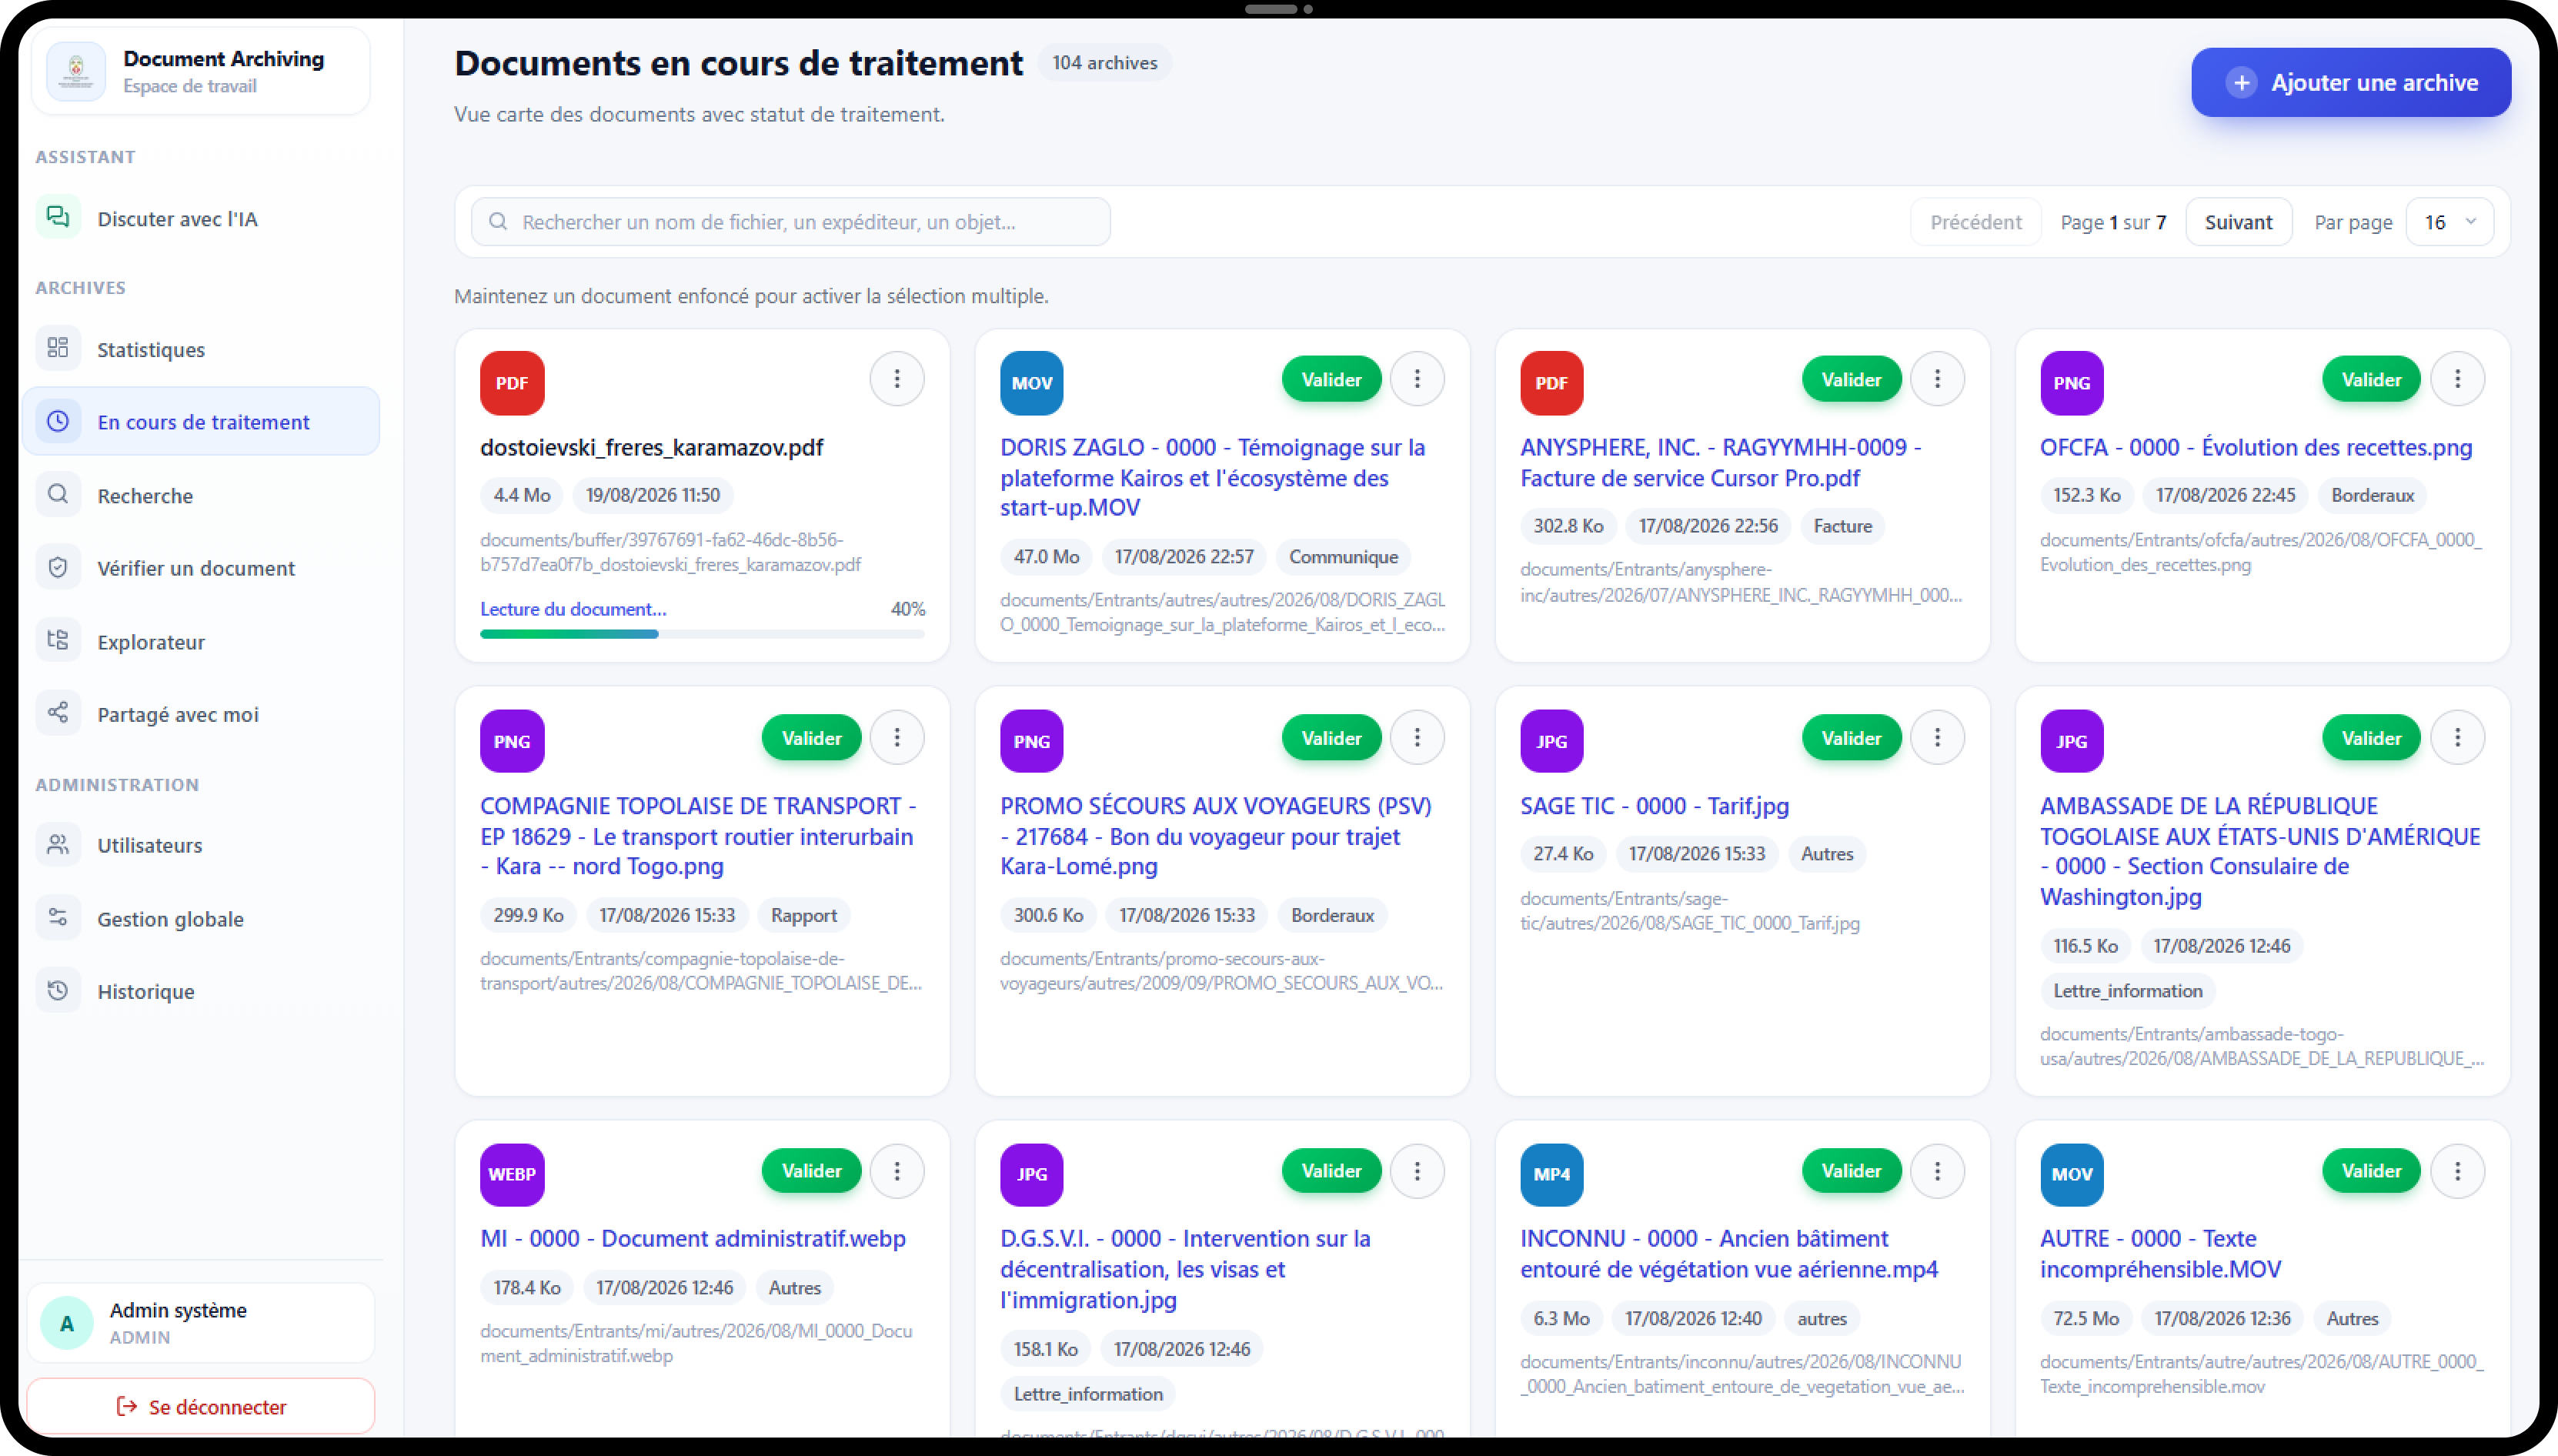
\includegraphics[width=0.98\textwidth]{images/screens/Traitement_documents.png}
\caption{Interface de traitement et de validation d'un document}
\label{fig:ui-traitement-validation}
\end{figure}

L'interface d'exploration documentaire reprend l'organisation retenue pour le classement, avec les niveaux Entrants, Sortants ou Internes, puis expéditeur, type documentaire, année et mois (figure~\ref{fig:ui-exploration}). Elle permet ainsi de retrouver les documents selon une logique proche de l'arborescence définie lors de la conception.

\begin{figure}[H]
\centering
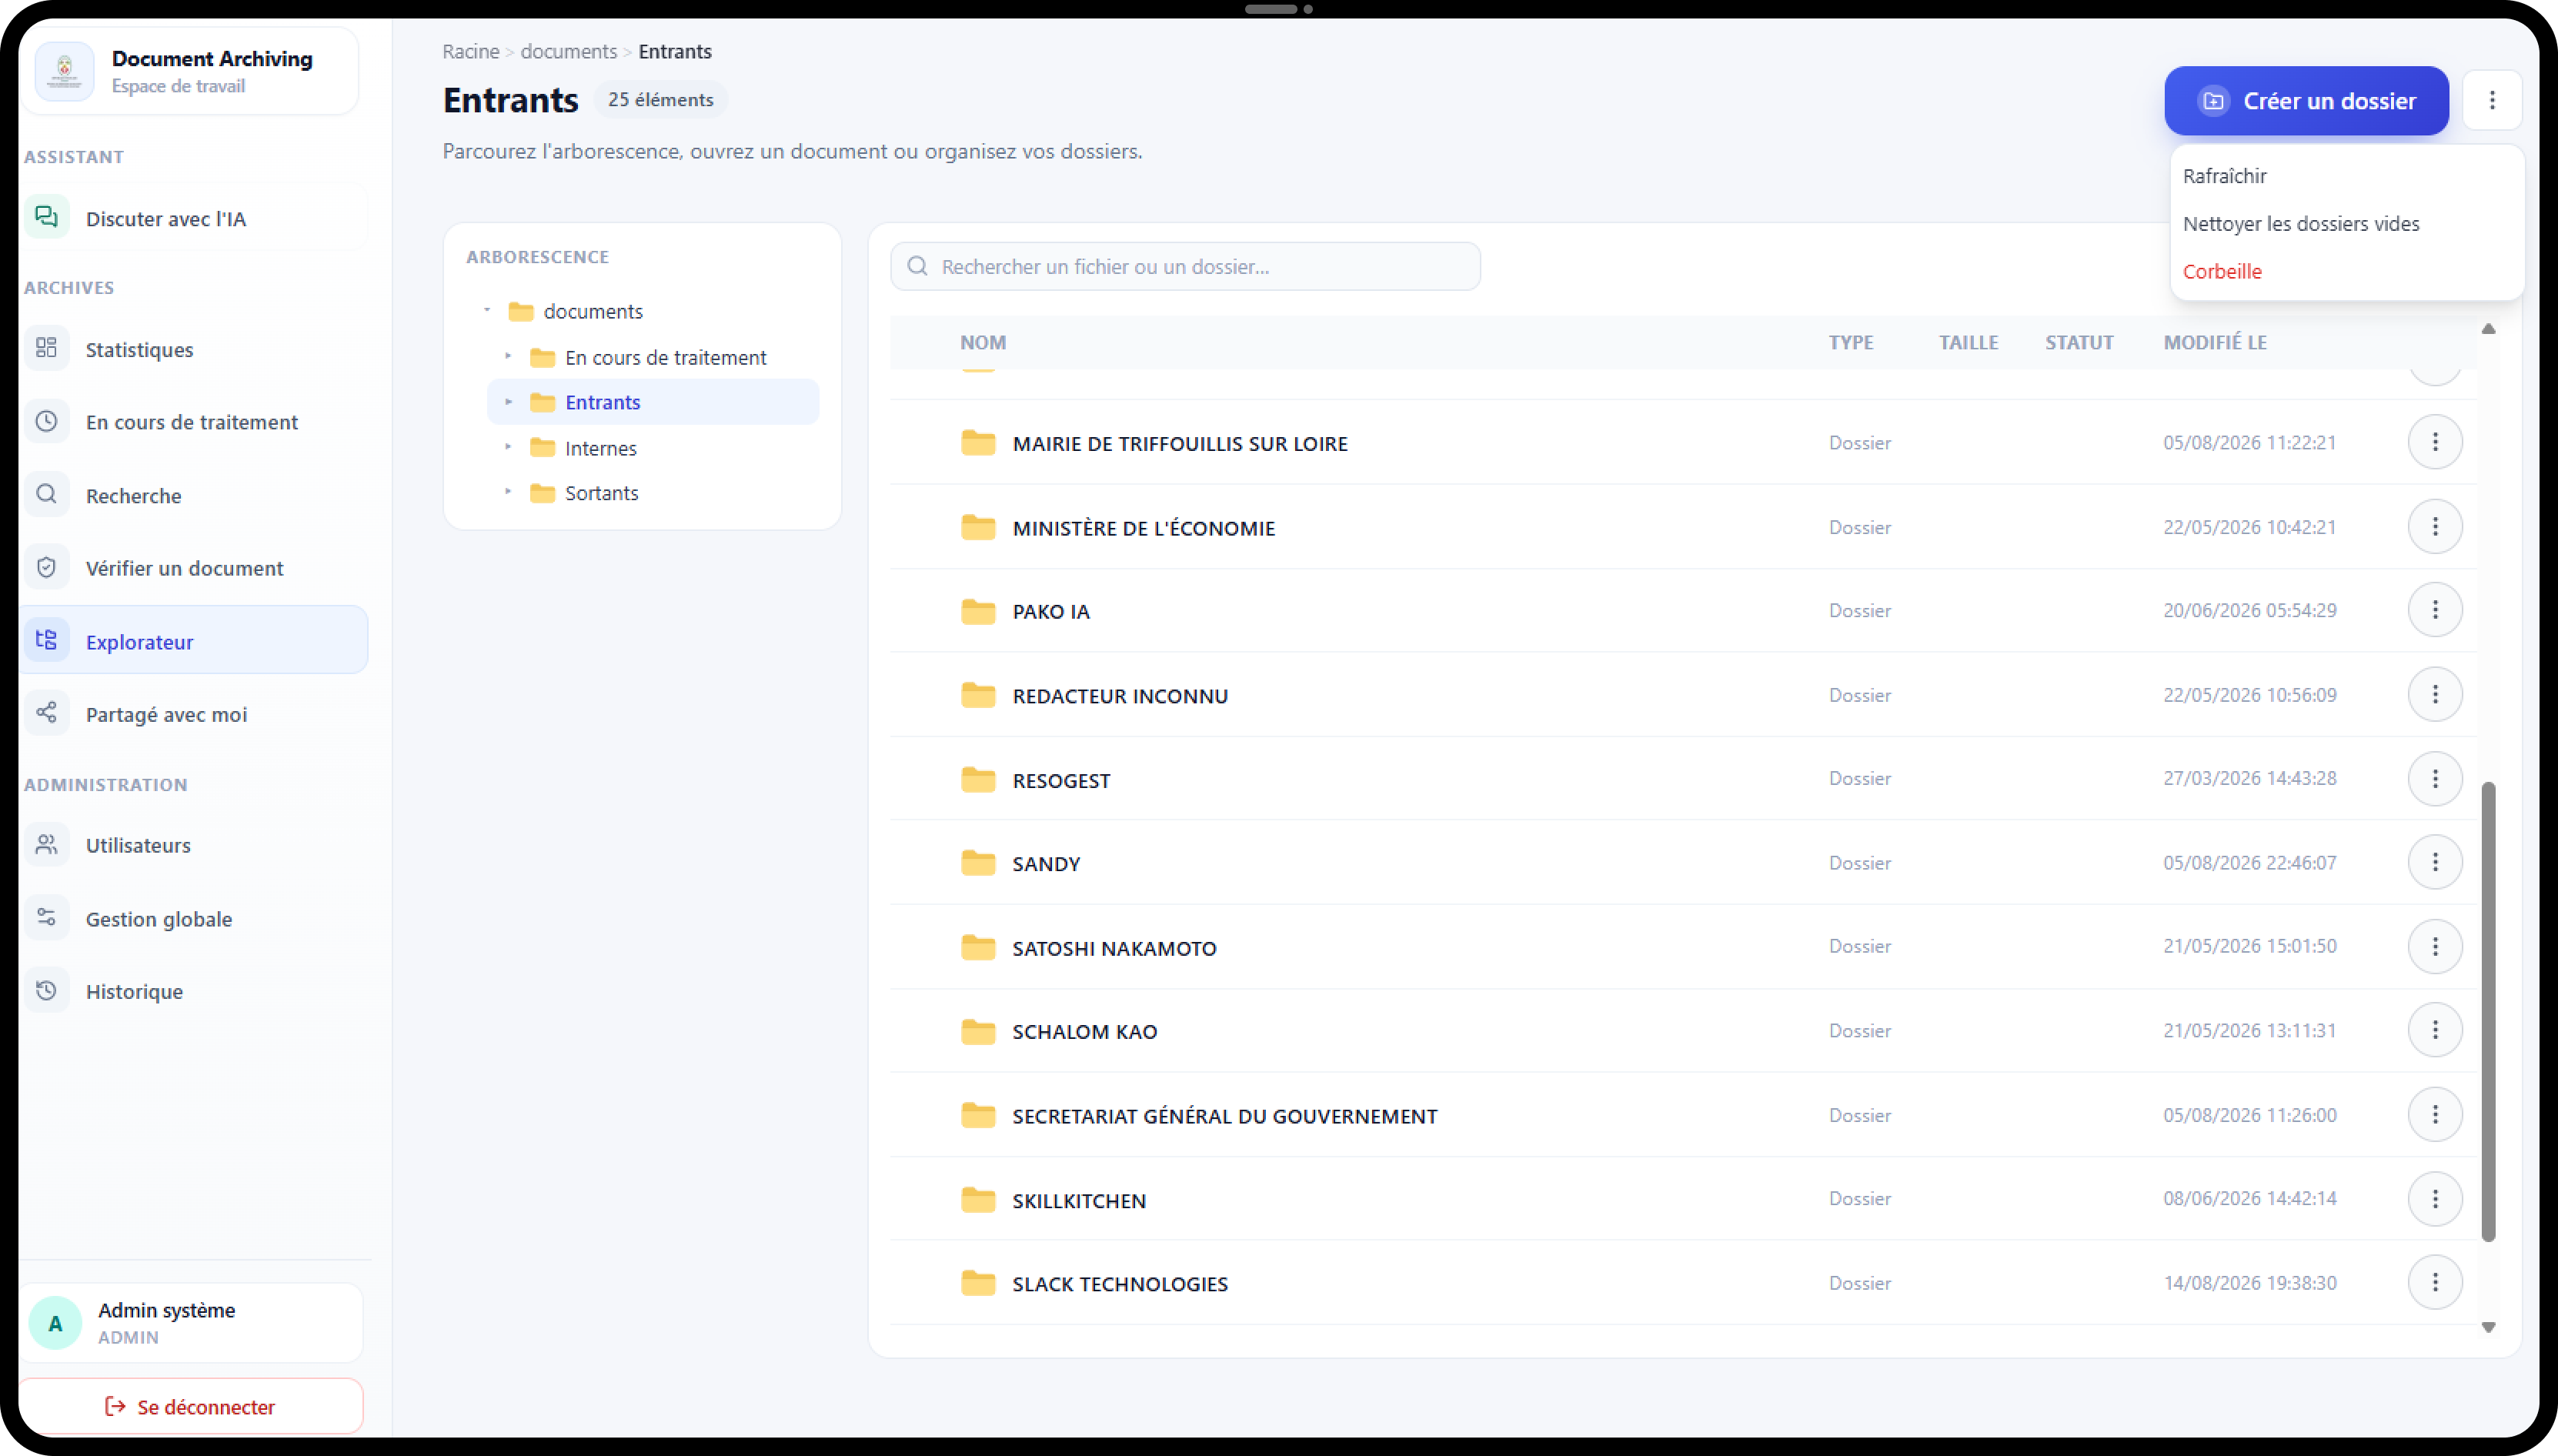
\includegraphics[width=0.98\textwidth]{images/screens/exploration_arborescence.png}
\caption{Interface d'exploration du fonds documentaire}
\label{fig:ui-exploration}
\end{figure}

La recherche et l'assistance intelligente constituent le second parcours majeur. L'utilisateur peut effectuer une recherche à partir de mots-clés et de filtres, ou formuler directement une question en langage naturel. Dans ce dernier cas, la réponse générée est accompagnée des sources utilisées, qui peuvent être ouvertes pour vérifier l'information fournie (figure~\ref{fig:ui-assistant}).

\begin{figure}[H]
\centering
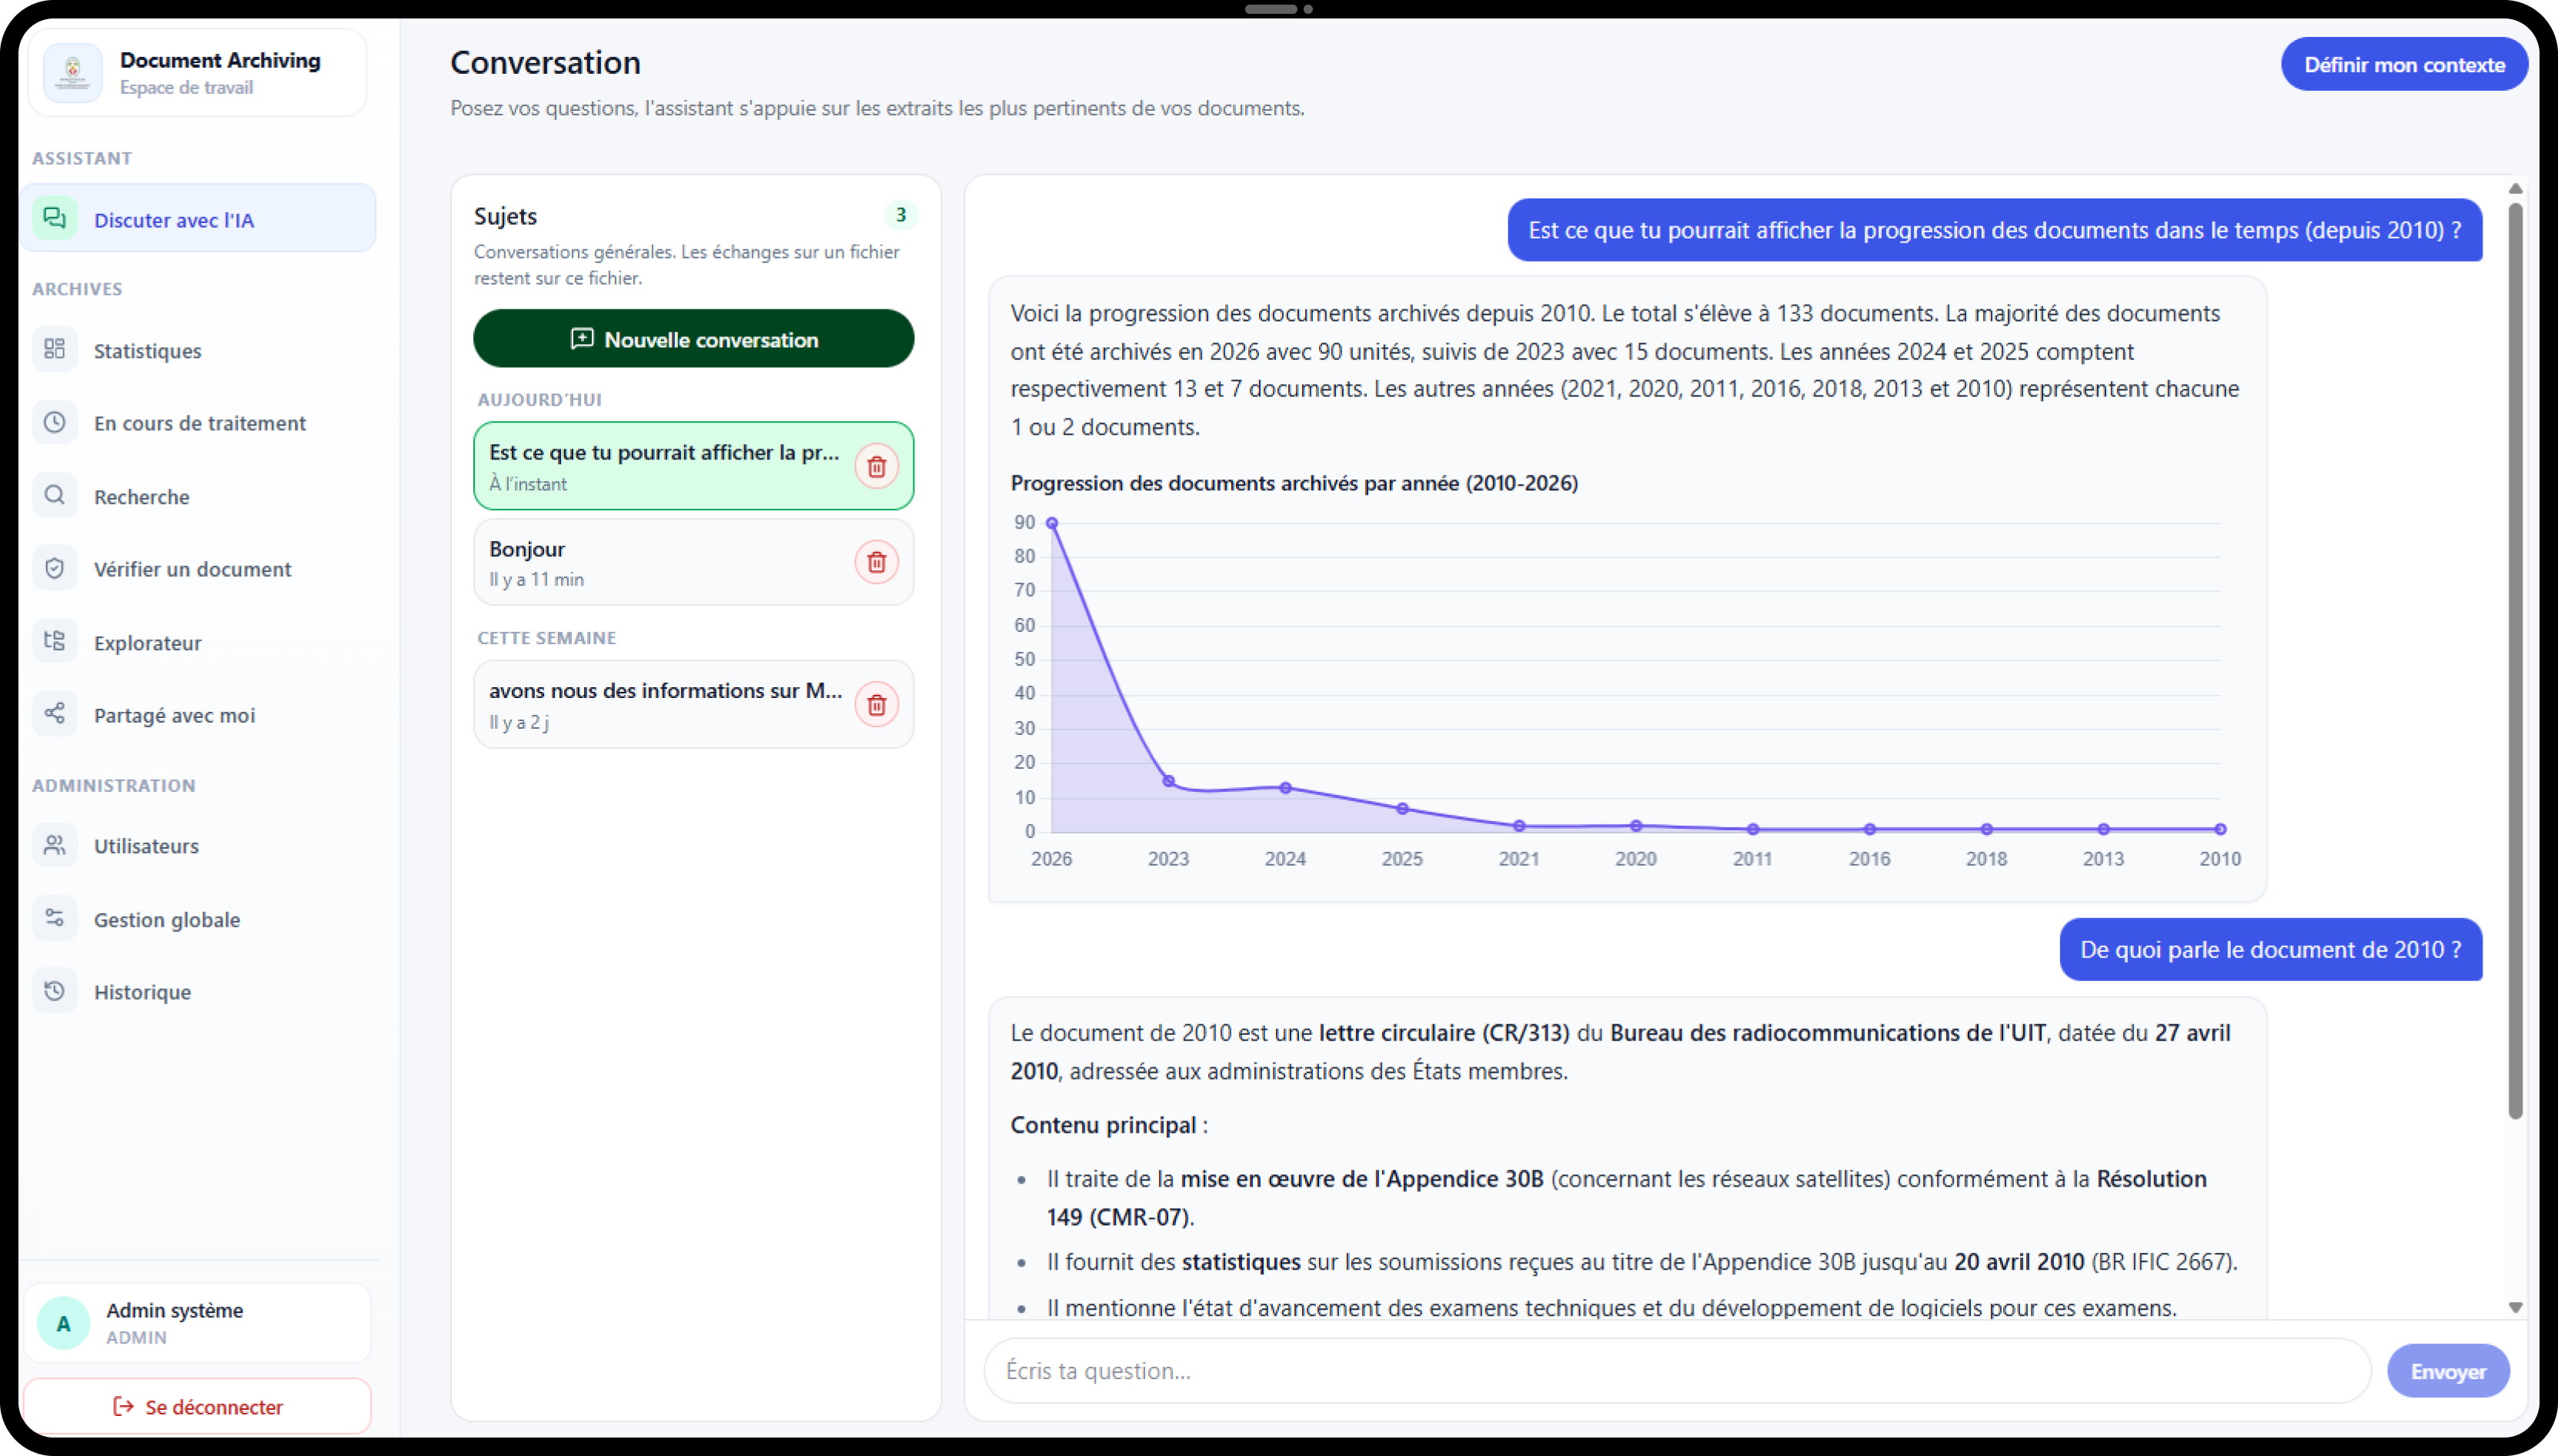
\includegraphics[width=0.98\textwidth]{images/screens/conversation_assistant.png}
\caption{Interface de recherche et d'assistance intelligente}
\label{fig:ui-assistant}
\end{figure}

Enfin, une vue synthétique de l'administration ou du suivi de l'activité illustre les fonctions de gouvernance et de supervision de la plateforme (figure~\ref{fig:ui-dashboard}).

\begin{figure}[H]
\centering
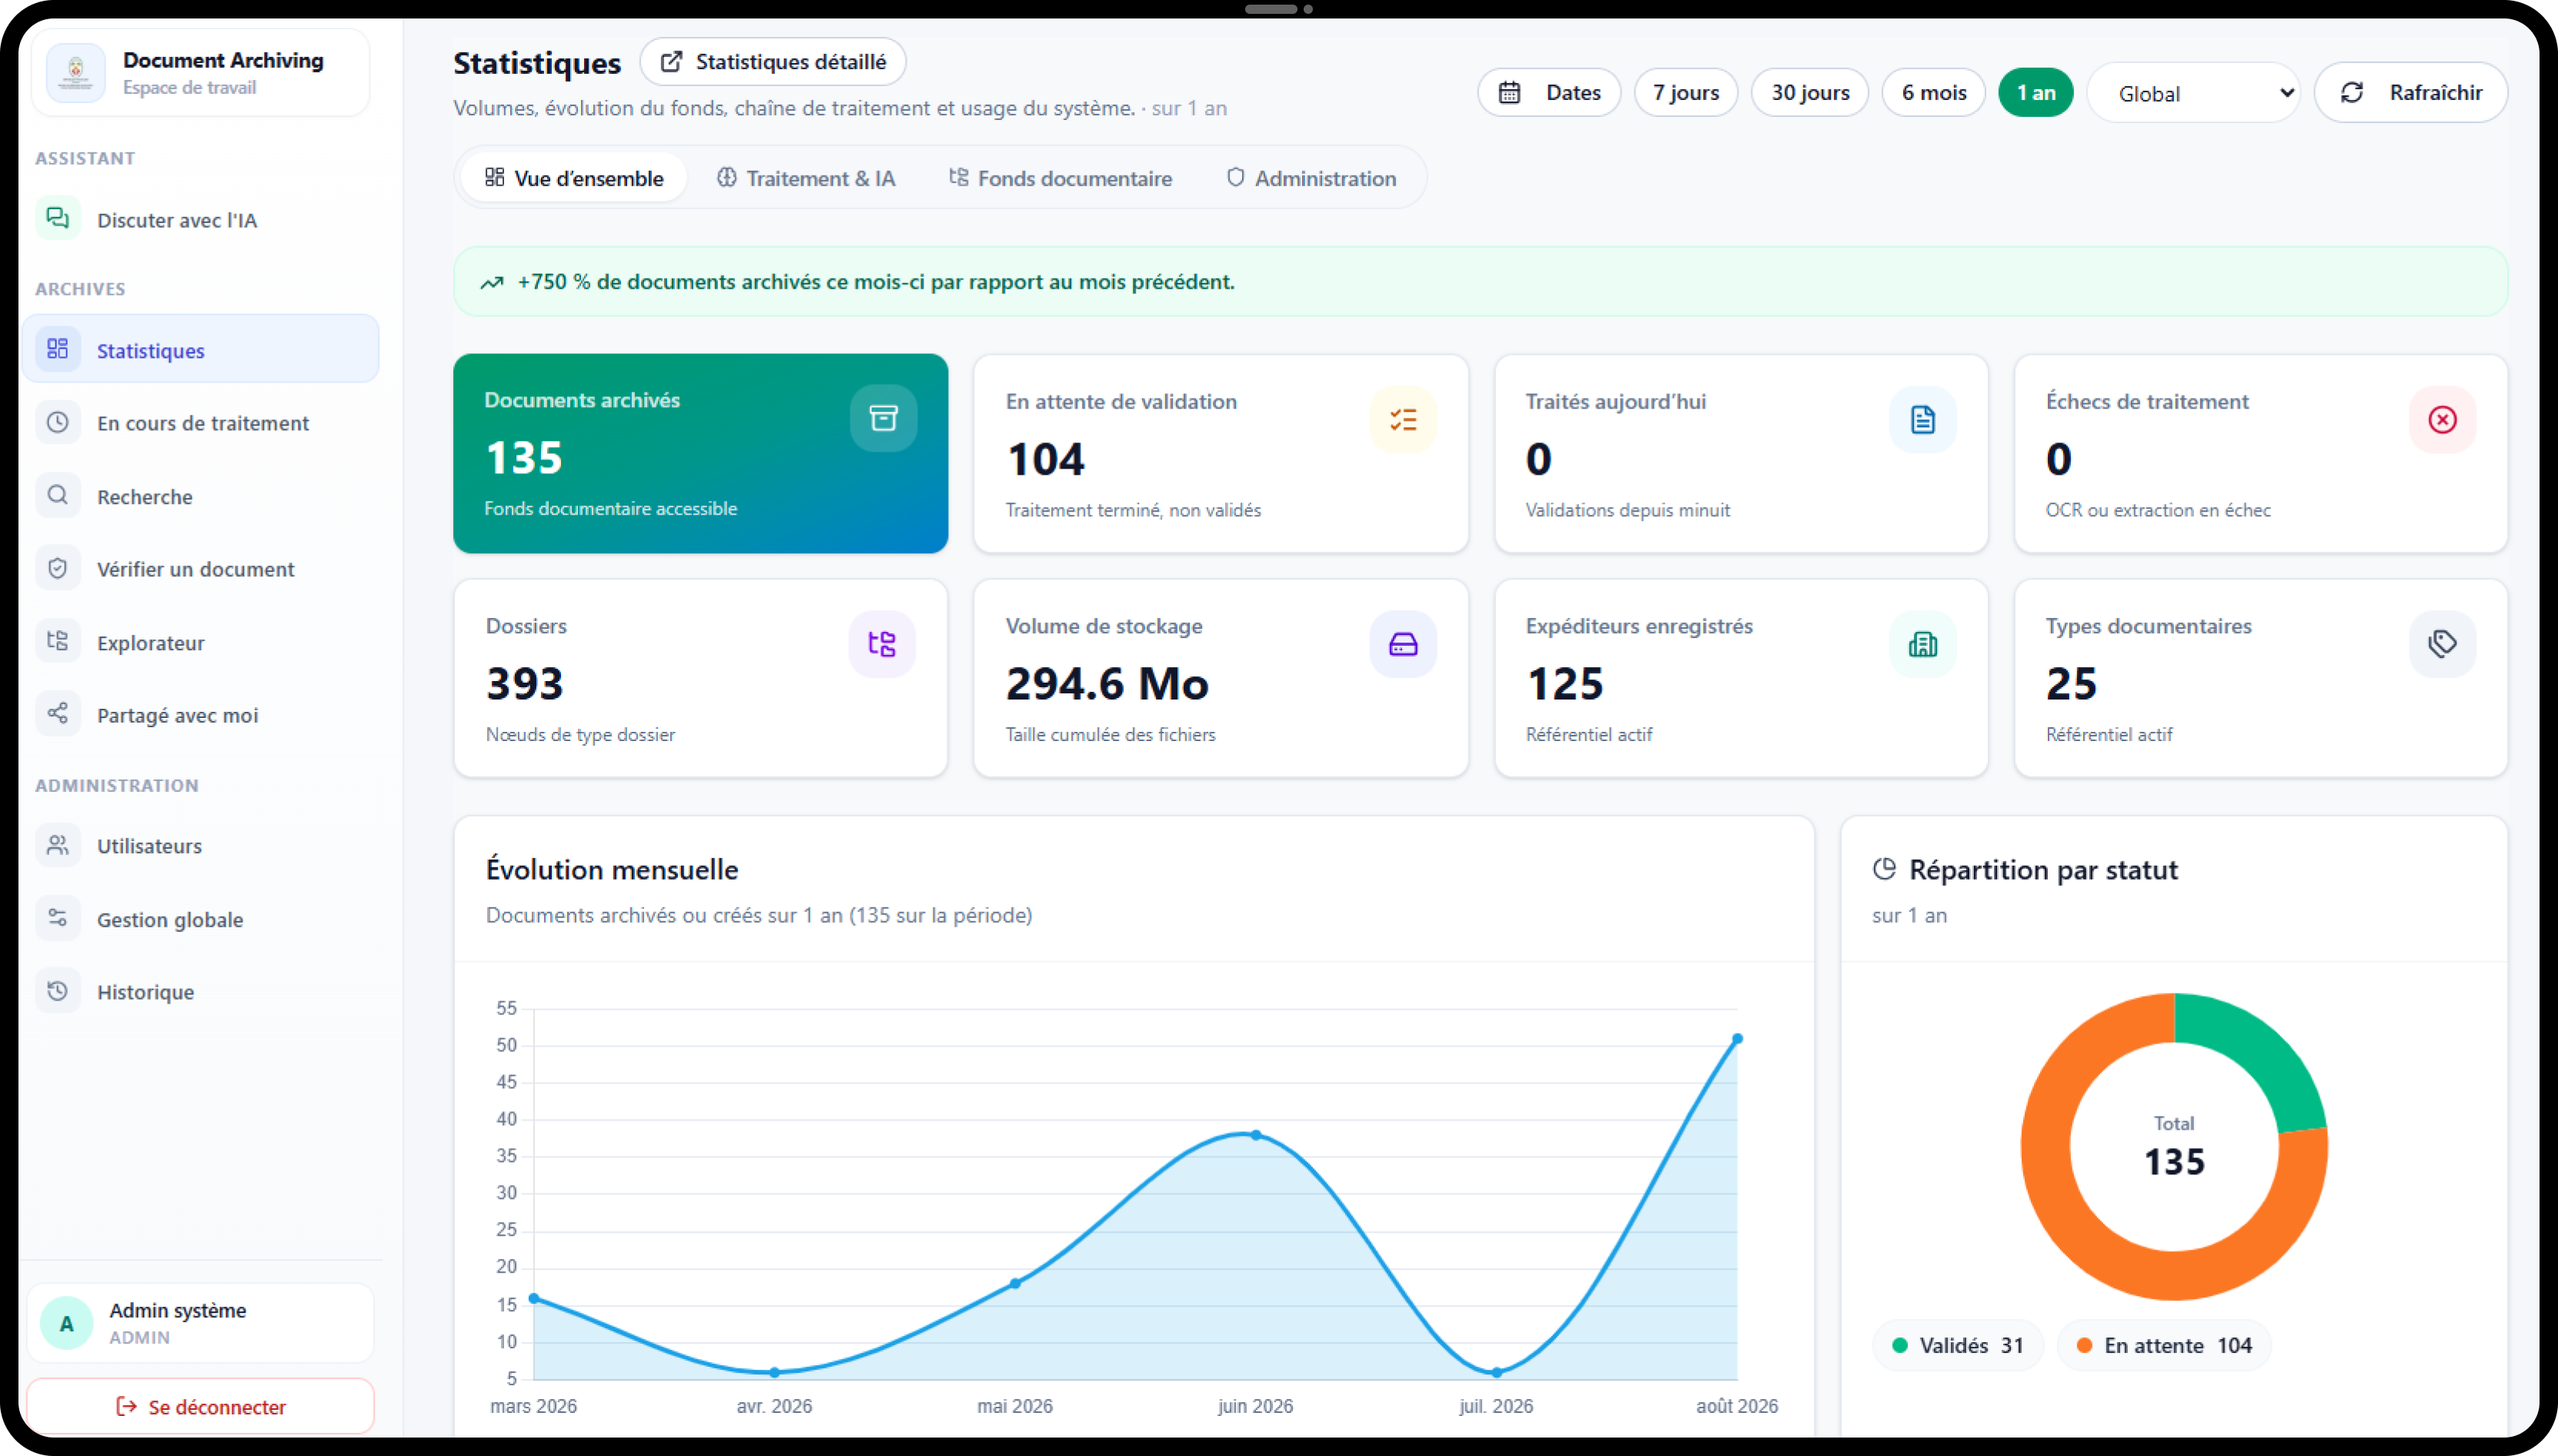
\includegraphics[width=0.98\textwidth]{images/screens/dashboard.png}
\caption{Tableau de bord de supervision de la plateforme}
\label{fig:ui-dashboard}
\end{figure}

Ces parcours traduisent concrètement les choix du chapitre~\ref{ch:conception} : proposer puis valider, classer par règles explicites, rechercher autrement qu'en parcourant l'arbre, et n'afficher que ce que les droits autorisent.

\section{Expérimentations et évaluation}

La conception a volontairement laissé ouverts certains réglages fins, notamment la taille des segments, le nombre d'extraits récupérés, les seuils de similarité et le nombre d'itérations. Cette section confronte ces choix à la solution déployée en environnement interne et revient sur la question posée au chapitre~\ref{ch:existant} : dans les conditions expérimentées, la solution répond-elle aux besoins identifiés ?

L'évaluation ne vise pas à multiplier les indicateurs. Elle les organise autour de quatre dimensions : la qualité du traitement, celle de l'OCR et de l'extraction, celle de la recherche, et celle du RAG. Elle ne constitue pas une preuve statistique généralisable à l'ensemble des archives administratives togolaises. Elle vise à caractériser le fonctionnement de la solution dans les conditions d'exploitation internes, en distinguant ce qui mesure réellement la question posée de ce qui n'en donne que l'apparence.

\subsection{Protocole, corpus et lecture des métriques}

Quatre ensembles doivent être distingués. Le \textbf{fonds historique} du ministère n'est pas mesuré ici dans son intégralité. Le \textbf{flux annuel} est estimé, d'après l'observation du service, à environ 10\,000 dossiers. Le \textbf{fonds accessible en production}, lu sur le tableau de bord le 26~août~2026, compte 35\,007 documents archivés. L'\textbf{échantillon d'évaluation} est un tirage stratifié de 300 documents parmi 34\,917 pièces éligibles (statut technique \texttt{done}, texte OCR ou segments disponibles), avec une graine fixée (\texttt{seed = 42}). Les métriques finales du harnais sont calculées sur le seul split de test ($n = 205$). Les 34\,917 pièces ne remplacent pas le fonds : elles en sont le sous-ensemble éligible au harnais (35\,007 $-$ 34\,917 $=$ 90 documents exclus par le filtre).

Le jeu de données de référence recopie les propositions déjà présentes en production. Les 300 documents ont été marqués comme validés pour le protocole, \textbf{sans relecture humaine des champs ni du texte OCR}. Les scores d'extraction, de type documentaire et d'OCR obtenus contre ce jeu de données de référence comparent donc le système à ses propres sorties. Ils ne sont pas reportés comme résultats : ils ne mesurent pas une performance métier. Les questions de recherche, une par document, ont été générées automatiquement à partir de l'objet et de l'expéditeur ; elles ne constituent pas un jeu métier relu par les agents. Un jeu de données de référence validé par des experts, plus fourni, sur le split de test (type, champs et extrait OCR), est prévu pour une campagne de mesures plus complète ; il n'est pas utilisé dans le présent mémoire.

Le moteur de recherche et l'assistant ont été interrogés en boucle locale sur le serveur de production. Dix objets MinIO de l'échantillon n'ont pas pu être copiés (clé absente ou chemin en base distinct de l'objet réel) ; ces absences limitent un rejeu OCR local, sans empêcher l'évaluation de l'extraction et de la recherche sur le reste du test.

Les paramètres retenus (tableau~\ref{tab:params-rag-realisation}) confirment, en exploitation, les valeurs de conception du tableau~\ref{tab:params-rag-conception} et de l'équation~\eqref{eq:rrf}. Ils ne prétendent pas à un optimum théorique, ni à une généricité hors de ce contexte.

\begin{table}[htbp]
\centering
\caption{Paramètres de travail de la solution déployée (recherche et indexation)}
\label{tab:params-rag-realisation}
\small
\renewcommand{\arraystretch}{1.45}
\begingroup
\rowcolors{2}{black!3}{white}
\begin{tabularx}{\textwidth}{@{}>{\bfseries}Y Y@{}}
\toprule
\rowcolor{black!12}
\tableheader{Paramètre} &
\tableheader{Valeur retenue} \\
\midrule
Taille d'un segment de contenu & environ 2000 caractères \\
Chevauchement & 400 caractères \\
Champs métier exploités & objet, expéditeur, type, destinataire, numéro interne \\
Modèle d'embeddings (local) & MiniLM multilingue, 384 dimensions \\
Fusion & RRF, $k=60$ (non calibré sur le test) \\
Nombre d'extraits (chat) & 8 \\
Statuts du corpus RAG par défaut & VALIDATED (hors DRAFT et corbeille) \\
Passe élargie si vide & implémentée, non isolée dans l'évaluation \\
\bottomrule
\end{tabularx}
\endgroup
\end{table}

\subsection{Qualité du traitement}

Le tableau de bord de production, au 26~août~2026, décrit l'échelle du fonds déjà archivé : 35\,007 documents. Sur ce stock, les trois étapes automatiques (OCR, extraction, analyse par modèle de langage) ont été menées à terme ; 32\,452 pièces sont validées (92,7~\%) et 2\,555 restent en file humaine (7,3~\%). Ces deux effectifs s'ajoutent au fonds : $32\,452 + 2\,555 = 35\,007$. Ce compteur n'est pas un taux d'échec nul du pipeline. En exploitation, sur le flux de traitement, le taux d'échec moyen observé est d'environ 5~\% : texte OCR inexploitable, timeout du modèle de langage, copie objet refusée, fichier isolé dans le répertoire d'erreur, nécessité d'un retraitement. Cette estimation est tirée des journaux Loki des services de traitement et des fichiers isolés dans le répertoire d'erreur du \texttt{scan-listener} ; le dénominateur est le nombre de documents soumis à la chaîne, et non le stock déjà archivé (35\,007) ni l'échantillon du harnais. Le harnais, calculé sur 300 documents déjà en statut \texttt{done}, ne capture pas ces échecs d'entrée ; il décrit la robustesse une fois la chaîne achevée, non le taux d'échec du flux réel.

Ces chiffres mesurent le fonctionnement technique du pipeline, non la justesse des métadonnées. Ils répondent toutefois à un besoin central du chapitre~\ref{ch:existant} : un volume annuel de l'ordre de 10\,000 dossiers ne peut plus reposer sur une saisie unitaire si la chaîne casse trop souvent. Un taux d'échec moyen d'environ 5~\%, avec reprise prévue (répertoire d'erreur, \texttt{reprocess}), reste compatible avec une exploitation interne ; il n'autorise pas à parler d'une chaîne sans défaillance.

Le tableau de bord fournit aussi un \textbf{taux de complétude} des métadonnées, distinct d'un taux de précision. Les propositions de l'IA atteignent une complétude moyenne d'environ 99~\% (100~\% sur les documents déjà validés). Le destinataire est le champ le plus souvent vide côté IA (97,8~\%). Un expéditeur faux mais renseigné compte comme complet : cet indicateur dit seulement si le champ est rempli.

\subsection{Qualité de l'OCR, de la classification et de l'extraction}

Sur le split de test ($n = 205$), le harnais a bien comparé le texte OCR, le type documentaire et les champs extraits aux valeurs déjà stockées en production. Comme le jeu de données de référence recopie ces sorties, le système est comparé à lui-même. Aucun score d'accuracy, de F1 ou de CER/WER n'est donc publié pour cette dimension : un chiffre, même imparfait, y serait lu comme une performance.

Un rejeu Tesseract sur cinq documents, confronté à l'OCR déjà en base, donne un CER moyen de 0,594 et un WER moyen de 0,699. Ce n'est pas un score humain : il mesure l'écart entre un Tesseract local et le texte déjà stocké. Il montre surtout qu'un jeu de données de référence validé par des experts serait nécessaire pour calibrer le moteur. Les temps OCR retenus pour le choix de Tesseract restent des ordres de grandeur observés sur le matériel cible, de l'ordre de 0,8 à 1,5~s par page, et non un engagement de service.

Tant qu'une annotation humaine du test n'est pas disponible, le tableau principal ne porte donc, pour cette dimension, que le temps moyen par page à titre indicatif et la complétude des métadonnées. L'accuracy, le F1 macro, le F1 d'extraction et le CER/WER de qualité n'y figureront qu'après relecture des références.

Les observations de terrain restent utiles pour interpréter ces limites. La qualité de l'OCR paraît liée à celle du scan : un courrier contrasté donne souvent un texte exploitable ; une page sombre, tamponnée ou manuscrite peut produire un OCR pauvre. Le garde-fou heuristique évite de transmettre ce bruit au classifieur. Un repli vers un modèle de vision a, dans certains cas, amélioré la transcription, au prix d'un temps plus élevé. Les erreurs rencontrées lors des essais portent notamment sur des organismes aux libellés proches, une source mal tranchée et des dates ambiguës ; le tableau de bord signale d'ailleurs des millésimes aberrants à nettoyer. Ces cas justifient le maintien de la validation humaine.

\subsection{Qualité de la recherche}

Ce volet est le plus crédible du lot : on compare des identifiants retournés par le service de recherche de production à l'identifiant du document pertinent, et non un champ à lui-même. Les 205 questions du split de test sont toutefois générées automatiquement (objet et expéditeur), ce qui borne l'interprétation.

Le rappel au rang~5 vaut 0,620 : environ 62~\% des questions ramènent le bon document dans les cinq premiers résultats. Le rappel au rang~10 est identique, ce qui indique que, lorsque le document est trouvé dans le haut de liste, il l'est déjà dans le top~5. Le MRR vaut 0,597 : lorsqu'il est trouvé, le document pertinent apparaît en moyenne vers le rang~1. Le nDCG au rang~5 vaut 0,603. Ces trois métriques suffisent pour le tableau principal. La précision aux rangs~5 et~10 (0,124 et 0,062) est mathématiquement cohérente avec un seul document pertinent par requête, mais beaucoup moins intuitive pour le lecteur ; elle n'est pas reprise dans la synthèse.

La latence du moteur, mesurée sur ces 205 requêtes, s'établit à 0,588~s en moyenne et 0,703~s au 95\textsuperscript{e}~percentile. Le maximum (1,342~s) est trop sensible à une requête exceptionnelle pour figurer dans le tableau principal. Pour un service interactif, le p95 sous la seconde est l'indicateur le plus utile.

Ces mesures ne remplacent pas le constat qualitatif déjà formulé lors des essais : une recherche uniquement dense peut manquer un numéro interne, une recherche uniquement lexicale une formulation proche ; la fusion RRF, alimentée aussi par le plein texte et les métadonnées, réduit ces angles morts dans le cadre observé. Huit extraits, avec une limite par document, restent un compromis de configuration, non un optimum démontré.

\subsection{Qualité du RAG}

Le rappel du contexte récupéré, calculé selon le protocole RAGAS \citp{es2024}{Es et al., 2024} sur les 205 questions, vaut 0,838. Il mesure la couverture des passages par rapport à une référence de contexte, et non la \og qualité RAG\fg{} globale. Il ne se confond pas avec le rappel documentaire au rang~5 (0,620) : l'un porte sur des extraits, l'autre sur l'identifiant du document.

La précision de contexte n'a pas pu être calculée (valeur non définie), faute de réponse de référence fournie au juge automatique. Ce n'est pas une métrique de performance ; c'est un état du protocole. De même, une mesure de similarité avec une réponse de référence telle que ROUGE-L \citp{lin2004}{Lin, 2004} et le taux d'ancrage des réponses dans les extraits récupérés (\textit{grounded rate}) n'ont pas été collectés pour ce jeu de 205 questions, bien que l'assistant de production ait été la cible des appels. Ils manquent au tableau principal. Une latence de génération moyenne et au p95 compléterait ce volet ; elle n'est pas reportée ici faute de série transmise.

L'assistant reste donc évalué, à ce stade, par la couverture du contexte récupéré, par les sources affichées dans l'interface, et par la consigne de ne pas compléter une réponse hors extraits. Ce n'est pas encore une mesure de la qualité des réponses générées.

\subsection{Choix des briques OCR et modèle de langage}
\label{sec:eval-choix-briques}

Une comparaison interne a permis de figer le moteur d'OCR et le modèle de langage local. Les temps indiqués sont des ordres de grandeur observés sur le matériel cible, non des engagements de service. Aucune note qualitative par étoiles n'est retenue : le critère déterminant est l'alignement avec un déploiement local, un coût nul à la page, et une latence compatible avec l'usage interactif.

\begin{table}[htbp]
\centering
\caption{Comparaison des moteurs d'OCR examinés (ordres de grandeur)}
\label{tab:choix-ocr}
\small
\renewcommand{\arraystretch}{1.40}
\begingroup
\rowcolors{2}{black!3}{white}
\begin{tabularx}{\textwidth}{@{}>{\bfseries}L{3.4cm}YYY@{}}
\toprule
\rowcolor{black!12}
\tableheader{Solution} &
\tableheader{Temps moyen} &
\tableheader{Déploiement} &
\tableheader{Coût} \\
\midrule
Tesseract~5 & $\sim$0,8--1,5~s/page & local & gratuit \\
EasyOCR & $\sim$3--8~s/page & local & gratuit \\
Moteurs cloud examinés & $\sim$1--4~s/page & distant & payant \\
\bottomrule
\end{tabularx}
\endgroup
\end{table}

Les moteurs cloud examinés (Google Cloud Vision, Azure AI Document Intelligence, AWS Textract) sont en général plus précis sur les scans difficiles, mais imposent un coût à la page, une sortie des documents hors du SI et une dépendance réseau. EasyOCR reste local, au prix d'un débit nettement inférieur pour un gain de précision limité dans le cadre observé. Tesseract~5 a été retenu : local, gratuit, de l'ordre d'une seconde par page, ressources faibles, cohérent avec un fonds de 35\,007 documents. Le rejeu CER/WER sur cinq pages n'invalide pas ce choix ; il rappelle seulement qu'un jeu de données de référence validé par des experts resterait nécessaire pour juger la précision réelle.

\begin{table}[htbp]
\centering
\caption{Comparaison des modèles de langage locaux examinés (Ollama)}
\label{tab:choix-llm}
\small
\renewcommand{\arraystretch}{1.40}
\begingroup
\rowcolors{2}{black!3}{white}
\begin{tabularx}{\textwidth}{@{}>{\bfseries}L{3.6cm}YYYY@{}}
\toprule
\rowcolor{black!12}
\tableheader{Modèle} &
\tableheader{Contexte} &
\tableheader{Temps moyen} &
\tableheader{Ressources} &
\tableheader{Local} \\
\midrule
Llama~3 (8B) & 8K & $\sim$1--3~s & faibles & oui \\
Mistral~7B & 32K & $\sim$2--4~s & faibles & oui \\
GPT-OSS~20B & 128K & $\sim$8--15~s & élevées & oui \\
Qwen3-Coder~30B & 256K & $\sim$17--23~s & élevées & oui \\
\bottomrule
\end{tabularx}
\endgroup
\end{table}

Llama~3 est plus léger, mais le contexte de 8K pèse pour l'extraction et le chat sur dossiers. GPT-OSS et Qwen3-Coder tiennent de plus longs contextes ; un éventuel avantage en raisonnement n'a pas été mesuré dans ce mémoire. Leur latence et leur empreinte mémoire restent, en l'état, incompatibles avec le chat interactif sur le serveur disponible. Mistral~7B tient le compromis retenu : 32K de contexte, quelques secondes par appel, ressources faibles, déploiement entièrement local.

\subsection{Réponse aux besoins du chapitre~\ref{ch:existant}}

Les quatre dimensions se relient aux besoins identifiés après l'analyse de l'existant. Le tableau~\ref{tab:besoins-realisation-ch5}, présenté dans la synthèse du chapitre, rassemble pour chaque besoin la réalisation correspondante et les constats issus de l'évaluation. Le tableau~\ref{tab:eval-systeme} en extrait les métriques conservées dans le résultat principal.

\section{Synthèse}

La conception présentée au chapitre~\ref{ch:conception} a été traduite en une plateforme fonctionnelle déployée en environnement interne. La solution assiste le traitement documentaire depuis l'acquisition jusqu'à la validation humaine, en combinant reconnaissance du contenu, extraction, analyse par intelligence artificielle, proposition de métadonnées, classement déterministe et indexation pour la recherche. Le modèle multi-composante est matérialisé par l'association du stockage objet et de la base de données relationnelle ; le pipeline asynchrone assure l'enchaînement des traitements ; le dispositif de recherche combine plusieurs modes de récupération avant de solliciter le modèle de langage. Les mécanismes de contrôle d'accès, de sensibilité, de journalisation et d'intégrité sont intégrés au fonctionnement de la plateforme.

Le tableau~\ref{tab:eval-systeme} rassemble les métriques dont la lecture est défendable dans l'état actuel du jeu de référence et des logs. Il n'inclut ni les scores d'exactitude obtenus contre les sorties de production, ni la précision au rang~$k$, ni une latence maximale, ni des indicateurs RAG non calculés.

\begin{table}[htbp]
\centering
\caption{Évaluation du système : métriques retenues pour le résultat principal}
\label{tab:eval-systeme}
\small
\renewcommand{\arraystretch}{1.40}
\begingroup
\rowcolors{2}{black!3}{white}
\begin{tabularx}{\textwidth}{@{}L{3.3cm}Y>{\raggedleft\arraybackslash}p{2.7cm}@{}}
\toprule
\rowcolor{black!12}
\tableheader{Dimension} &
\tableheader{Métrique} &
\tableheader{Résultat} \\
\midrule
Robustesse & Documents traités & 35\,007 \\
 & Taux d'échec moyen (exploitation) & $\approx$~5~\% \\
OCR & Temps moyen par page & $\sim$0,8--1,5~s \\
Extraction & Complétude moyenne (propositions IA) & 99~\% \\
Recherche & MRR & 0,597 \\
 & Rappel au rang~5 & 0,620 \\
 & nDCG au rang~5 & 0,603 \\
 & Latence moyenne & 0,588~s \\
 & Latence p95 & 0,703~s \\
RAG & Rappel du contexte récupéré & 0,838 \\
\bottomrule
\end{tabularx}
\endgroup
\end{table}

N'entrent pas dans ce tableau, faute de vérité terrain validée par des experts ou de série transmise : le CER et le WER de qualité, l'accuracy et le F1 macro de classification, le F1 d'extraction, ROUGE-L, le taux d'ancrage des réponses générées, et la latence de l'assistant. Ce n'est pas un vide de protocole : c'est la limite honnête de ce qui peut être affirmé aujourd'hui.

Le tableau~\ref{tab:besoins-realisation-ch5} relie ensuite ces résultats aux besoins du chapitre~\ref{ch:existant}.

\begin{table}[htbp]
\centering
\caption{Besoins identifiés, réalisation et observations issues de l'évaluation}
\label{tab:besoins-realisation-ch5}
\small
\renewcommand{\arraystretch}{1.45}
\begingroup
\rowcolors{2}{black!3}{white}
\begin{tabularx}{\textwidth}{@{}>{\bfseries}Y Y Y@{}}
\toprule
\rowcolor{black!12}
\tableheader{Besoin identifié au chapitre~\ref{ch:existant}} &
\tableheader{Réalisation} &
\tableheader{Observation} \\
\midrule
Réduire le traitement manuel &
Proposition automatique de métadonnées et de classification ; traitement asynchrone &
35\,007 documents traités ; taux d'échec moyen d'environ 5~\% en exploitation ; complétude IA d'environ 99~\% ; une correction humaine reste nécessaire avant validation \\
Fiabiliser le classement &
Construction du chemin à partir des métadonnées validées et de règles déterministes &
Le classement ne dépend pas d'un chemin librement généré par le modèle de langage \\
Conserver le contrôle humain &
États \texttt{DRAFT} et \texttt{VALIDATED} ; validation par un agent &
32\,452 documents validés (92,7~\%) et 2\,555 en file humaine (7,3~\%), soit 35\,007 \\
Faciliter la recherche &
Recherche lexicale, dense et hybride ; RRF ; assistance conversationnelle sourcée &
Rappel au rang~5 de 0,620 et MRR de 0,597 sur 205 questions ; latence p95 de 0,703~s \\
Adapter la structure documentaire &
Référentiels administrables et racines Entrants, Sortants et Internes &
115 types et 13\,244 expéditeurs actifs ; la structure peut être adaptée sans modifier le principe du modèle \\
Sécuriser les archives &
RBAC, ACL, sensibilité, Keycloak et Vault ; filtrage avant récupération &
Le périmètre d'accès est pris en compte avant l'alimentation du contexte destiné au RAG \\
Assurer la traçabilité &
Journalisation des événements, suivi des traitements et empreinte SHA-256 &
Les propositions automatiques peuvent être distinguées des décisions et actions humaines \\
\bottomrule
\end{tabularx}
\endgroup
\end{table}

Au-delà des indicateurs, la solution déployée change le mode de traitement. L'agent n'a plus à renseigner systématiquement l'ensemble des informations avant de classer une pièce : il examine et corrige des propositions. Le classement est ensuite construit à partir des métadonnées retenues et de règles explicites. La recherche interroge le contenu, sous contrainte des droits, avec un rappel au rang~5 de 62~\% sur le jeu automatique du test. Ce n'est pas encore une preuve de qualité des types, des champs ou des réponses générées.

Ces résultats restent limités aux conditions d'exploitation internes et au protocole décrit. Ils ne permettent pas de généraliser un niveau de précision de l'OCR, de la classification ou de l'extraction à l'ensemble des archives administratives togolaises. Le chapitre suivant discute cette portée, les limites du jeu de référence et les perspectives d'une annotation humaine du split de test.


\chapter{Méthodologie et organisation du projet}
\section{Démarche}
Ce chapitre rappelle la démarche méthodologique adoptée pour la conduite du projet, depuis le cadrage initial jusqu'à la mise en production progressive de la solution.

Une approche itérative et incrémentale, inspirée des méthodes agiles (Scrum), a été retenue afin de livrer rapidement une première version fonctionnelle du système, puis d'enrichir progressivement ses fonctionnalités en fonction des retours des utilisateurs.

Cette démarche a permis de réduire les risques, d'améliorer l'adéquation aux besoins métiers et de favoriser une validation continue des choix techniques.

Les principales étapes ont été les suivantes :
\begin{itemize}
  \item \textbf{Cadrage fonctionnel} : recueil des besoins auprès des parties prenantes (secrétariats, équipe technique), identification des contraintes métier et définition des cas d'usage prioritaires ;
  \item \textbf{Prototypage initial} : mise en place d'un premier pipeline minimal (ingestion $\rightarrow$ OCR $\rightarrow$ stockage) afin de valider les choix techniques ;
  \item \textbf{Itérations successives} : ajout progressif des modules d'extraction, d'assistance intelligente (classification, renommage) et de recherche documentaire ;
  \item \textbf{Intégration des interfaces utilisateur} : développement des interfaces de consultation et de validation, avec prise en compte des retours terrain ;
  \item \textbf{Stabilisation et mise en production} : amélioration de la robustesse, mise en place de l'observabilité (logs, métriques, alertes) et préparation au déploiement en environnement \textit{on-premise}.
\end{itemize}

L'implication des parties prenantes a été un élément clé de la démarche. Des échanges réguliers avec les utilisateurs finaux ont permis d'ajuster les fonctionnalités, notamment sur les règles de classement et les interfaces de validation.

Les principaux risques identifiés concernaient :
\begin{itemize}
  \item la qualité et la variabilité des documents scannés (impact sur l'OCR) ;
  \item l'hétérogénéité des formats documentaires ;
  \item la nécessité de garantir un contrôle humain sur les décisions automatisées.
\end{itemize}

Ces risques ont été atténués par :
\begin{itemize}
  \item une architecture asynchrone basée sur un système de messagerie, permettant de fiabiliser le traitement ;
  \item la mise en place d'un workflow de validation utilisateur (\og proposer puis valider \fg{}) ;
  \item une approche progressive permettant d'ajuster les traitements en fonction des résultats observés.
\end{itemize}

\section{Organisation et planification}
Le projet a été structuré selon une logique d'itérations courtes (\textit{sprints}), avec des livraisons incrémentales permettant de valider rapidement les fonctionnalités développées.

Les principaux livrables ont été organisés comme suit :
\begin{itemize}
  \item (i) ingestion automatique des documents ;
  \item (ii) OCR et stockage ;
  \item (iii) extraction des informations et gestion des métadonnées ;
  \item (iv) assistance au classement et au renommage ;
  \item (v) interface utilisateur et moteur de recherche ;
  \item (vi) observabilité, supervision et durcissement du système.
\end{itemize}

Chaque itération donnait lieu à une démonstration auprès des utilisateurs et de l'équipe technique, permettant de recueillir des retours et d'ajuster les développements suivants. Cette boucle de feedback a contribué à améliorer progressivement la pertinence fonctionnelle et l'ergonomie du système.


\part{Exploitation, sécurité, évaluation et bilan}
\chapter{Observabilité et exploitation}
\section{Objectifs}
L’observabilité vise à donner une visibilité sur :
\begin{itemize}
  \item la santé des services ;
  \item les erreurs (OCR/extraction, erreurs HTTP) ;
  \item la latence et les volumes de requêtes ;
  \item les logs applicatifs (corrélation par service/conteneur).
\end{itemize}

\section{Tableaux de bord applicatifs}
En complément de la supervision technique (métriques et logs), l’application propose des tableaux de bord destinés au suivi opérationnel : volumes de documents, répartition par statuts, indicateurs de traitement et journaux d’actions.
\begin{figure}[h!]
\centering
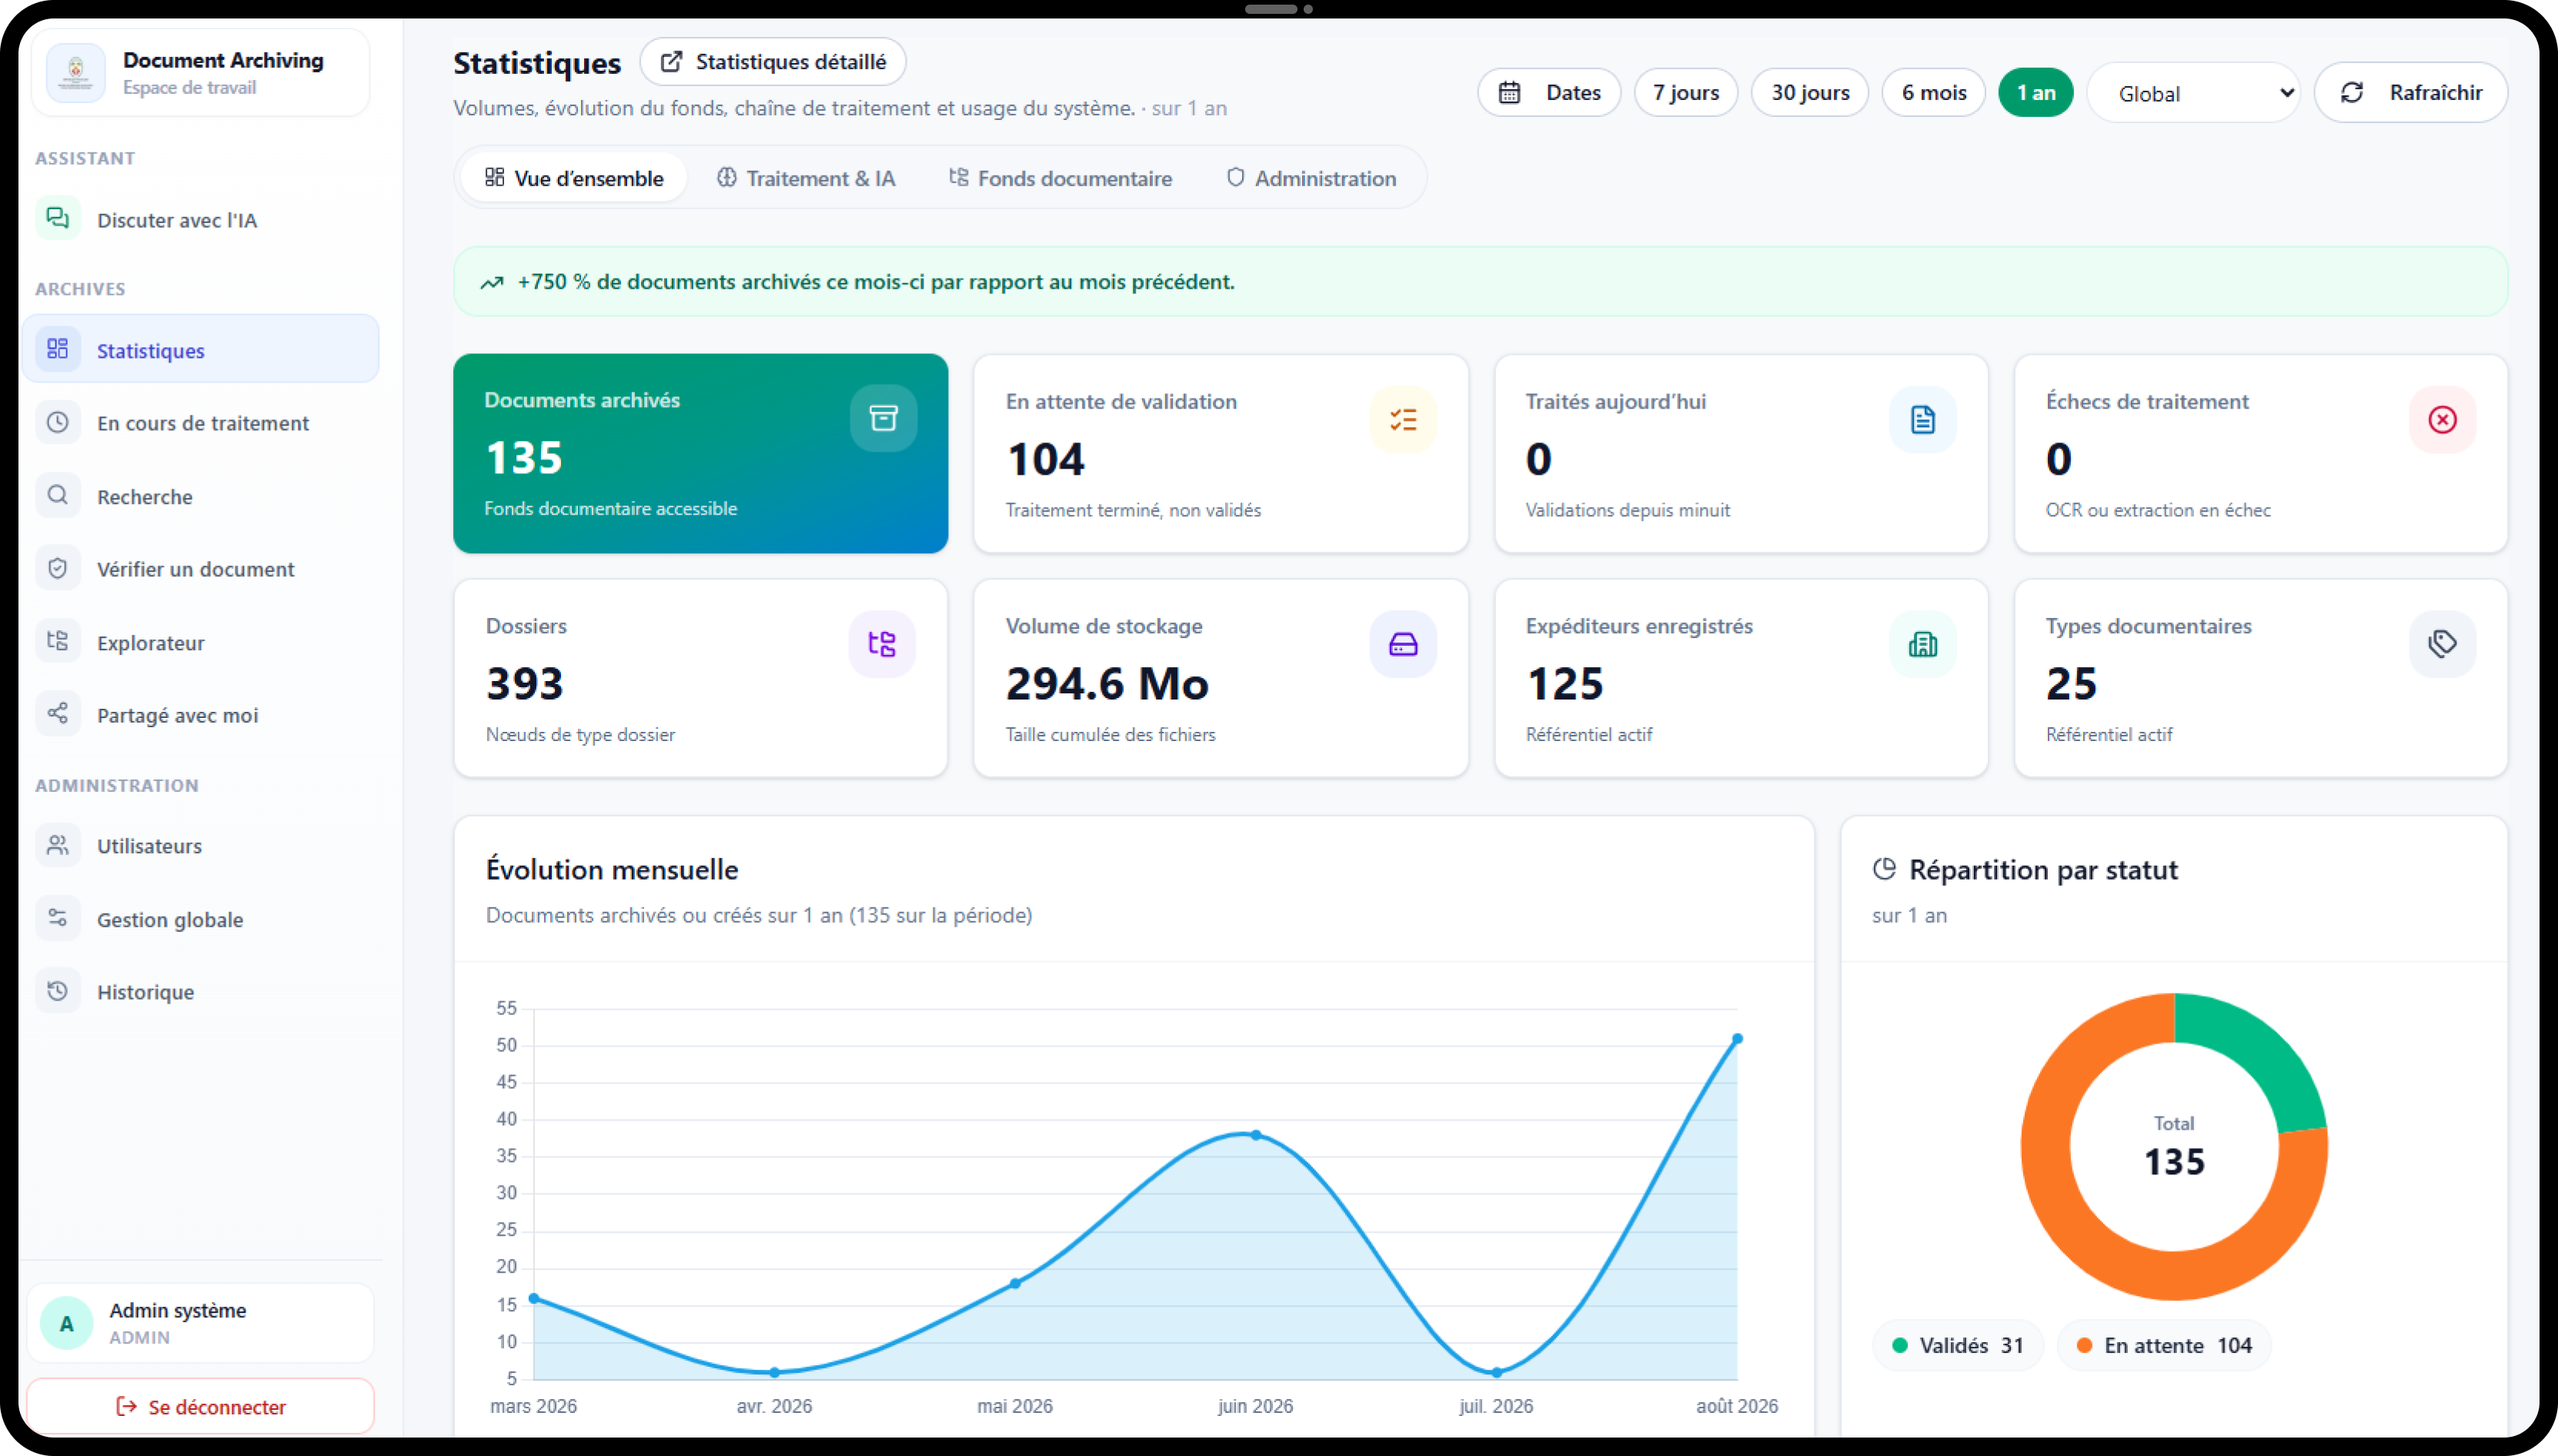
\includegraphics[width=0.98\textwidth]{images/screens/dashboard.png}
\par\vspace{0.6em}
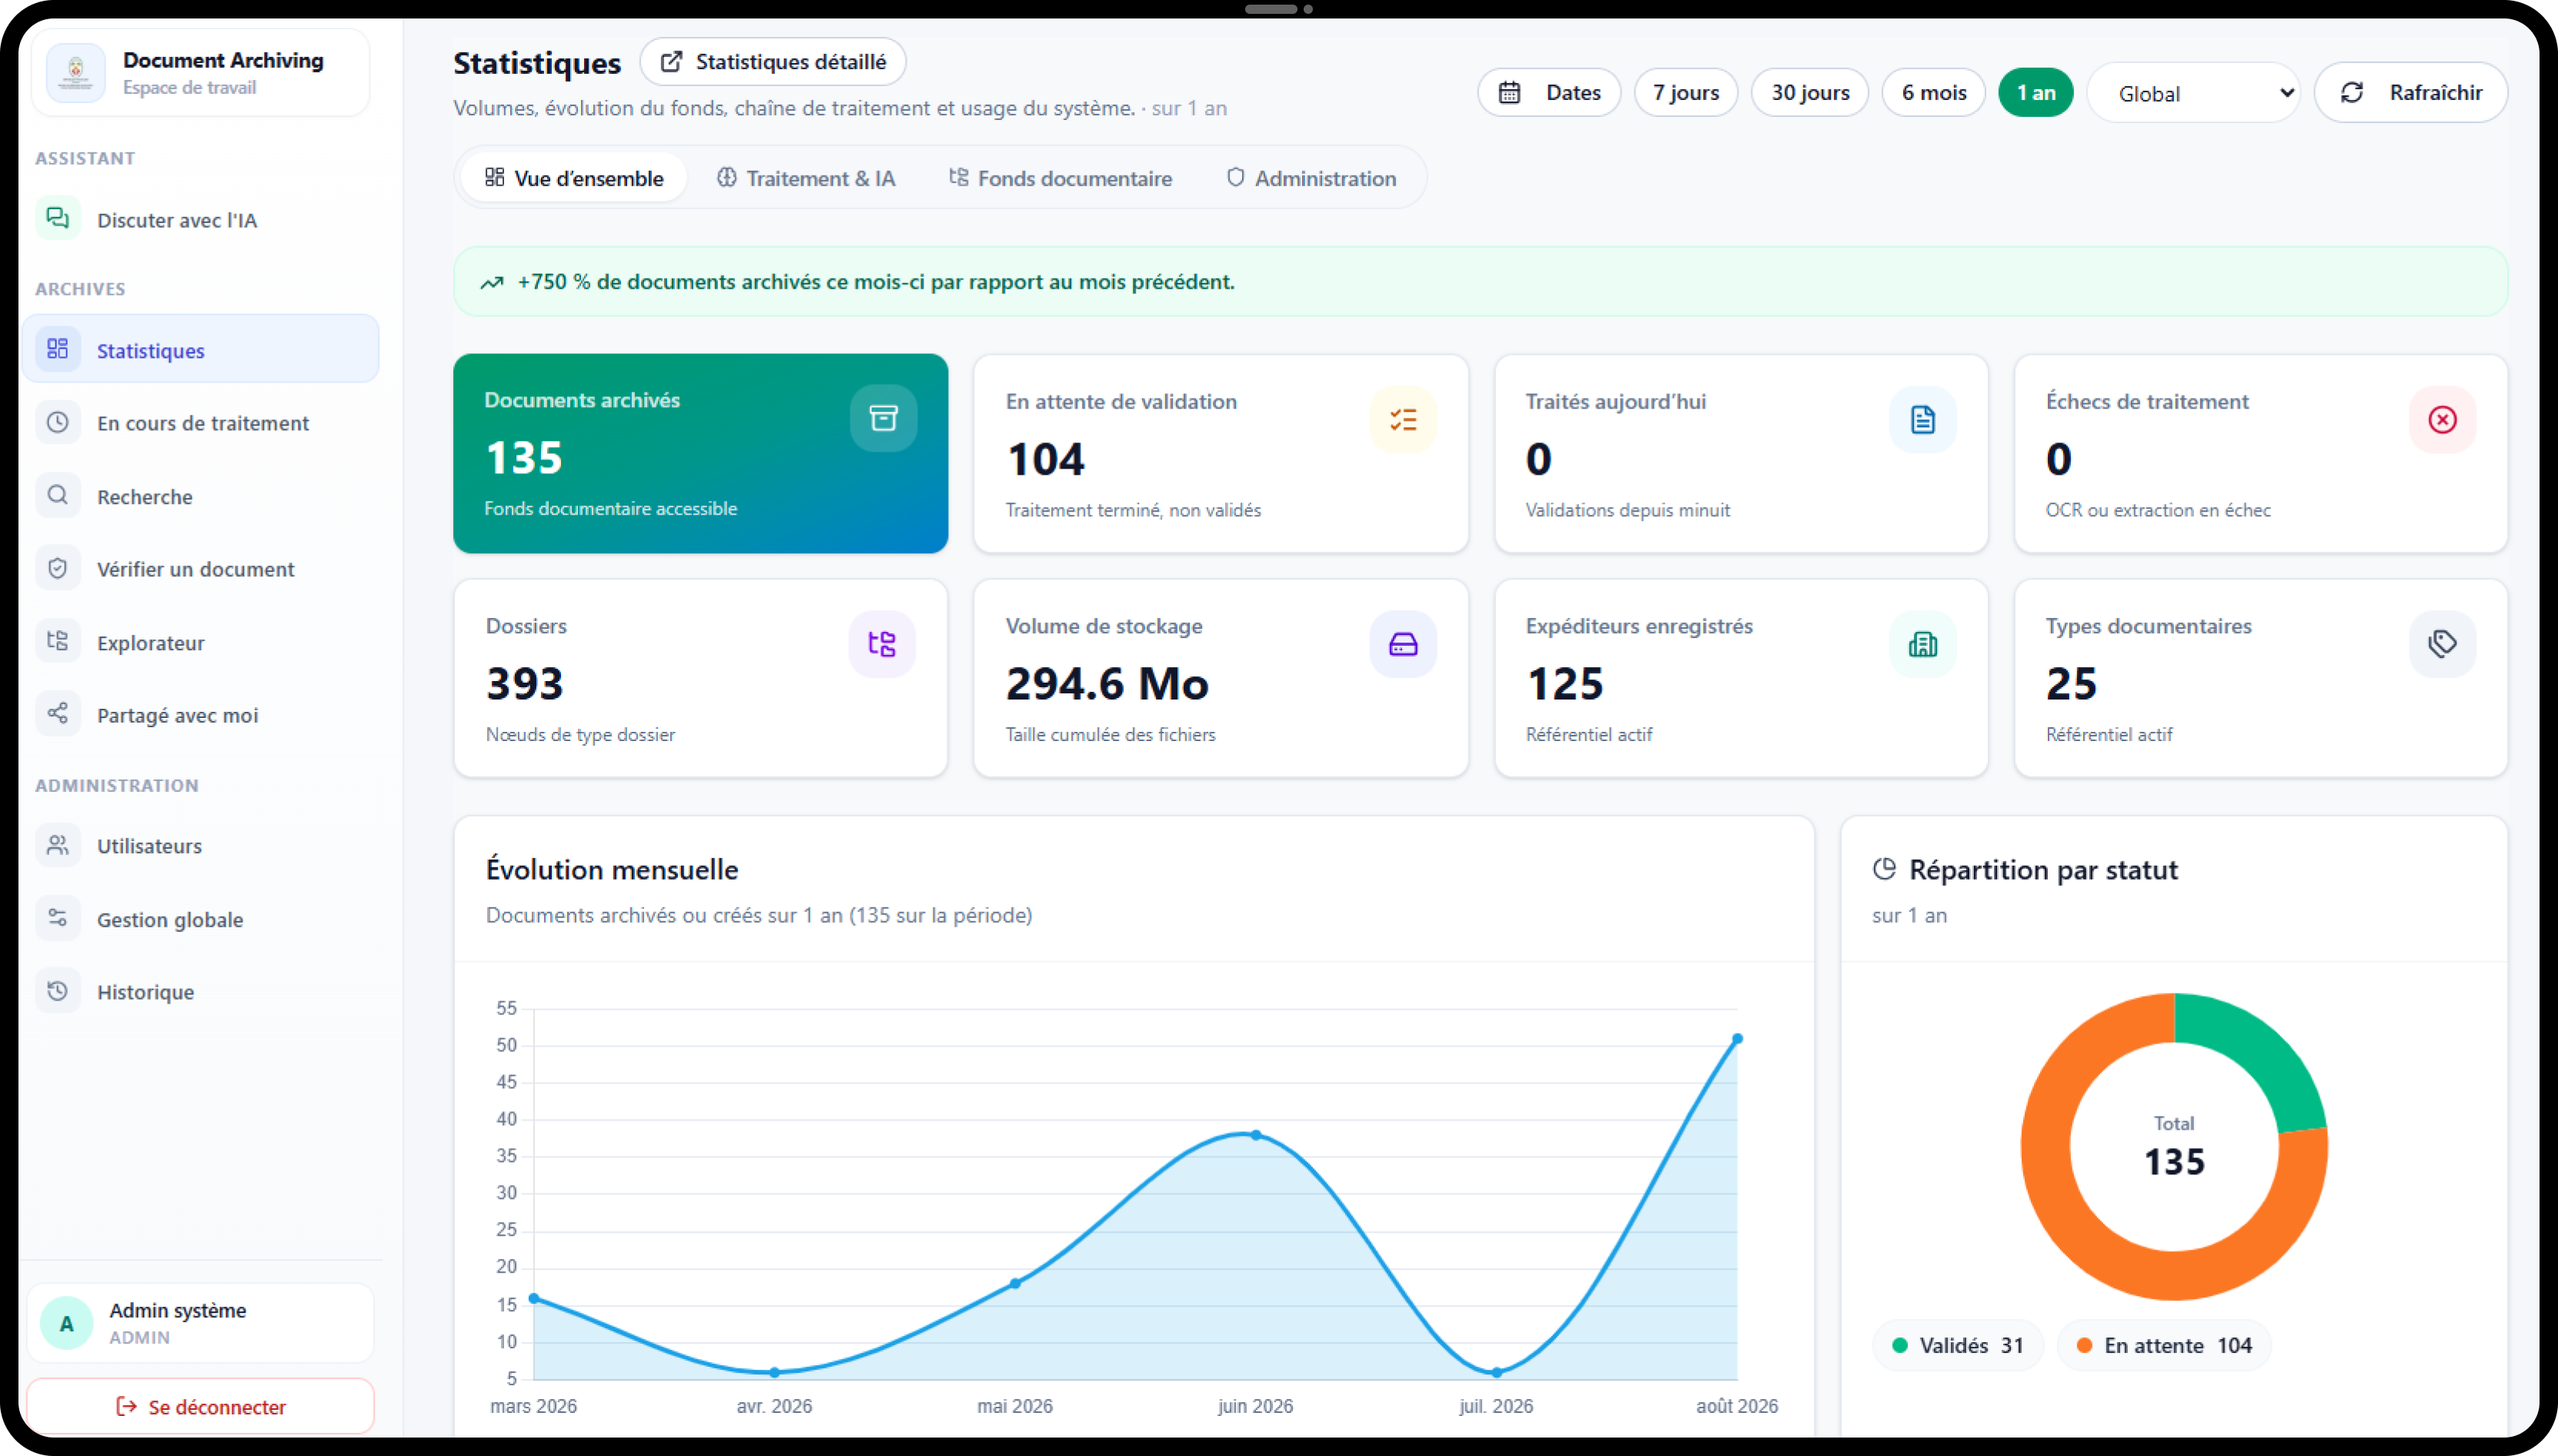
\includegraphics[width=0.98\textwidth]{images/screens/dashboard.png}
\caption{Tableaux de bord applicatifs : indicateurs de volumétrie, statuts, types de documents et temps moyen de traitement.}
\label{fig:dashboards-app}
\end{figure}

\section{Stack mise en place}
Une stack séparée est fournie :
\begin{itemize}
  \item \textbf{Prometheus} : collecte des métriques sur \texttt{/metrics} (FastAPI) et \texttt{/api/metrics} (Next.js) ;
  \item \textbf{Grafana} : dashboards et alerting, avec provisioning automatique ;
  \item \textbf{Loki} : stockage des logs ;
  \item \textbf{Vector} : collecte des logs Docker et expédition vers Loki.
\end{itemize}

\section{Alertes}
Des règles Prometheus détectent :
\begin{itemize}
  \item un taux d’erreurs HTTP 5xx supérieur à 5\% sur 10 minutes ;
  \item une latence p95 supérieure à 2s sur 10 minutes ;
  \item la présence d’erreurs OCR/extraction via des compteurs dédiés.
\end{itemize}

\chapter{Sécurité}
\section{Approche générale}
Le système est déployé \textbf{on-premise} afin de respecter les contraintes de souveraineté et de confidentialité propres à une administration publique. Dans ce contexte, l’architecture de sécurité s’inspire d’une approche \textbf{Zero Trust} : ne pas supposer qu’un réseau interne est sûr par défaut, limiter la surface exposée, vérifier systématiquement l’identité et appliquer des contrôles d’accès stricts.

\section{Exposition, réseau et segmentation}
L’exposition des composants est volontairement minimisée. Les accès externes sont concentrés sur un point d’entrée unique (reverse proxy), configuré en \textbf{TLS} afin de protéger les échanges. Les services internes (OCR, extraction, bus de messages, bases) restent non exposés et accessibles uniquement sur le réseau interne.

La segmentation réseau sépare les composants selon leur rôle (API/Frontend, traitements, stockage, observabilité, consoles). En production, les interfaces d’administration (RabbitMQ, MinIO, Grafana) sont restreintes (VPN, filtrage IP, comptes dédiés) afin d’éviter toute exposition accidentelle.

\section{Gestion des identités et des accès (IAM)}
La gestion des identités et des accès est un élément central pour sécuriser l’usage quotidien (secrétariats, administrateurs, services métier). Une intégration IAM est prévue via un fournisseur dédié (\textbf{Keycloak}) afin de :
\begin{itemize}
  \item centraliser l’authentification (\textbf{SSO}) et réduire la multiplication des comptes applicatifs ;
  \item gérer les rôles et groupes, et appliquer des politiques d’accès homogènes ;
  \item renforcer l’authentification (ex. \textbf{MFA}) selon la sensibilité des profils.
\end{itemize}
Cette approche facilite également la gestion du cycle de vie des comptes (création, révocation) et l’audit des connexions.

\section{Contrôle d’accès, RBAC et moindre privilège}
Le contrôle d’accès repose sur le principe du \textbf{moindre privilège} : chaque utilisateur et chaque service ne dispose que des droits strictement nécessaires. Le modèle RBAC (rôles et permissions) permet de limiter la consultation, la recherche et l’administration selon les profils, et de tracer les actions sensibles.

Au niveau des services, les permissions d’accès aux ressources (buckets MinIO, tables, files RabbitMQ) sont séparées et attribuées de manière fine, afin de réduire l’impact d’un éventuel compromis d’un composant.

\section{Gestion des secrets et configuration}
La configuration applicative est aujourd’hui centralisée via un fichier \texttt{.env} (développement). Pour une mise en production robuste, l’externalisation et la sécurisation des secrets est prévue avec \textbf{Vault} (HashiCorp Vault). L’objectif est d’éviter tout stockage en clair de mots de passe, clés API et tokens, et de permettre :
\begin{itemize}
  \item la rotation et la révocation des secrets ;
  \item la distribution contrôlée des secrets aux services autorisés ;
  \item la réduction du risque de fuite via les dépôts, logs ou sauvegardes.
\end{itemize}

\section{Traçabilité et journalisation}
La traçabilité est essentielle pour un environnement sensible : journalisation des actions (audit), suivi des traitements et corrélation des événements. Le système s’appuie sur :
\begin{itemize}
  \item un journal d’événements applicatifs (actions et changements d’état) ;
  \item des logs centralisés (Loki/Vector) et des métriques (Prometheus) pour détecter les anomalies ;
  \item des alertes (erreurs, latences, indisponibilités) afin de réduire le temps de réaction.
\end{itemize}
Ces mécanismes contribuent à la détection d’incidents, à l’analyse post-mortem et au respect des exigences d’audit.

\chapter{Bilan de la mission et recommandations}
\section{Livrables et résultats}
Ce chapitre dresse un bilan global de la mission, en présentant les réalisations concrètes, les limites rencontrées, ainsi que les recommandations pour une mise en production et les enseignements tirés sur le plan personnel.

Au cours de la mission, une solution complète d’archivage numérique a été conçue et implémentée. Les principaux livrables incluent :
\begin{itemize}
  \item un pipeline de traitement automatisé couvrant l’ingestion des documents, l’OCR, l’extraction d’informations et l’indexation ;
  \item une architecture microservices assurant la modularité et la scalabilité du système ;
  \item une interface web permettant la consultation, la recherche et la validation des documents ;
  \item un système de recherche combinant recherche plein texte et recherche sémantique ;
  \item un assistant conversationnel basé sur une approche \textit{RAG} pour faciliter l’accès à l’information ;
  \item un déploiement en environnement \textit{on-premise} via Docker Compose ;
  \item une première couche d’observabilité incluant logs, métriques et tableaux de bord.
\end{itemize}

Les résultats observés sur un échantillon représentatif montrent :
\begin{itemize}
  \item une réduction significative des tâches manuelles liées au tri et au renommage ;
  \item une amélioration de la cohérence et de la qualité du classement documentaire ;
  \item une meilleure traçabilité des opérations grâce à la journalisation ;
  \item un accès plus rapide à l’information via la recherche et le chat documentaire.
\end{itemize}

\section{Limites et difficultés rencontrées}
Malgré les résultats obtenus, plusieurs limites et difficultés ont été identifiées.

\textbf{Sur le plan technique :}
\begin{itemize}
  \item la qualité variable des scans a un impact direct sur les performances de l’OCR ;
  \item l’hétérogénéité des formats documentaires complique l’extraction et la structuration des données ;
  \item certains traitements (OCR, extraction, embeddings) peuvent être coûteux en temps et en ressources.
\end{itemize}

\textbf{Sur le plan opérationnel :}
\begin{itemize}
  \item l’intégration dans un environnement contraint (réseau interne, sécurité) a nécessité des ajustements ;
  \item la gestion des volumes importants de documents impose une optimisation continue des performances ;
  \item la nécessité de conserver une validation humaine limite l’automatisation complète du processus.
\end{itemize}

Ces contraintes ont conduit à des arbitrages, notamment :
\begin{itemize}
  \item le choix d’un traitement asynchrone pour améliorer la robustesse ;
  \item la mise en place d’un workflow de validation utilisateur pour garantir la fiabilité ;
  \item une approche progressive privilégiant la qualité des résultats plutôt que l’automatisation totale.
\end{itemize}

\section{Bilan personnel}
Cette mission m’a permis de développer des compétences techniques et méthodologiques significatives dans la conception et la mise en œuvre de systèmes distribués orientés traitement documentaire.

\textbf{Sur le plan technique,} j’ai approfondi :
\begin{itemize}
  \item le développement d’architectures microservices (API, communication asynchrone) ;
  \item l’intégration de briques d’intelligence artificielle (OCR, extraction, \textit{RAG}) ;
  \item le déploiement et l’exploitation de solutions en environnement \textit{on-premise} (Docker, supervision).
\end{itemize}

\textbf{Sur le plan méthodologique,} cette expérience m’a permis de :
\begin{itemize}
  \item adopter une démarche itérative inspirée des méthodes agiles ;
  \item collaborer étroitement avec des utilisateurs métiers afin de mieux comprendre leurs besoins ;
  \item intégrer des contraintes réelles (performance, sécurité, exploitation) dans la conception.
\end{itemize}

Enfin, cette mission a également mis en évidence des axes d’amélioration, notamment :
\begin{itemize}
  \item approfondir les aspects liés à la sécurité des systèmes distribués ;
  \item améliorer l’optimisation des performances sur des volumes importants ;
  \item renforcer les pratiques de pilotage de projet et de formalisation des besoins.
\end{itemize}

\chapter{Discussion}
Ce chapitre interprète les résultats obtenus au regard de la problématique initiale et des choix méthodologiques retenus.

\section{Interprétation des résultats}
Les livrables du projet montrent qu’il est possible d’industrialiser une chaîne d’archivage numérique sous contraintes \textit{on-premise}, en combinant OCR, extraction assistée par IA et validation humaine. La réduction des tâches manuelles de tri et de renommage, ainsi que l’amélioration de la cohérence du classement, confirment la pertinence d’une approche « proposer puis valider ». L’accès accéléré à l’information via la recherche sémantique et le chat documentaire répond directement à l’enjeu d’exploitabilité des archives numérisées.

\section{Limites de l’interprétation}
Plusieurs limites appellent à la prudence. La qualité de l'OCR demeure dépendante de la qualité des scans ; les performances observées sur un échantillon ne se généralisent pas automatiquement à l'ensemble du fonds documentaire. Les expérimentations du chapitre~5 confirment l'intérêt opérationnel de l'assistant, tout en restant pour partie qualitatives : une évaluation automatique plus large du RAG demeure un prolongement possible. Enfin, le maintien d'une validation humaine, nécessaire à la fiabilité, freine une automatisation totale : ce n'est pas un échec, mais un arbitrage assumé entre efficacité et contrôle.

\section{Apports au regard de la problématique}
La problématique posée en introduction trouve une réponse opérationnelle : une chaîne d’archivage numérique peut traiter un volume important de documents, réduire les interventions manuelles, améliorer le classement, garantir la traçabilité et offrir une recherche fiable, à condition de déployer une architecture résiliente, des règles métier explicites et un workflow de validation. Les perspectives (référentiels documentaires, gouvernance, optimisation RAG, signature électronique) prolongent cette réponse vers une industrialisation plus poussée.

\chapter*{Conclusion et perspectives}
\addcontentsline{toc}{chapter}{Conclusion et perspectives}
Le système développé constitue une chaîne d’archivage numérique complète, couvrant l’ensemble du cycle de vie du document, depuis la collecte automatique des scans jusqu’à leur consultation et leur recherche. En réduisant significativement les opérations manuelles (tri, renommage, saisie) et en proposant un classement plus homogène, la solution améliore à la fois la qualité de l’archivage et les délais de traitement.

Le choix d’un déploiement en environnement \textit{on-premise} permet de répondre aux exigences de sécurité et de souveraineté propres au contexte administratif, tandis que l’intégration de mécanismes d’observabilité contribue à une exploitation fiable et maîtrisée du système au quotidien. Par ailleurs, l’apport de techniques d’intelligence artificielle, notamment pour l’extraction d’informations et la recherche sémantique, renforce l’accessibilité et la valorisation du patrimoine documentaire.

Néanmoins, ce projet constitue une première étape vers un système d’archivage pleinement industrialisé. Plusieurs axes d’évolution peuvent être envisagés afin d’en améliorer la robustesse, la pertinence et l’intégration métier.

Les perspectives principales concernent :
\begin{itemize}
  \item l’amélioration des règles métier de classement, à travers la formalisation de référentiels documentaires, de modèles de nommage et la gestion des cas particuliers ;
  \item le renforcement des workflows de validation et de la gouvernance documentaire (gestion des droits, circuits de traitement, versioning) ;
  \item l’amélioration des capacités de recherche et d’assistance documentaire, notamment par l’optimisation des approches \textit{RAG} (qualité des contextes, citations, gestion des permissions) ;
  \item l’intégration de fonctionnalités complémentaires telles que la signature électronique, les politiques de conservation ou encore des tableaux de bord décisionnels.
\end{itemize}

À terme, l’évolution de ce système pourrait s’inscrire dans une démarche plus large de transformation numérique, visant à faire de la gestion documentaire un levier stratégique d’efficacité et de valorisation de l’information au sein de l’administration.

\chapter*{Références}
\addcontentsline{toc}{chapter}{Références}

Les références sont regroupées par thème. La numérotation reste continue, afin de conserver les renvois du corps du mémoire.

\subsubsection*{Archives et gestion documentaire}
\begin{enumerate}[leftmargin=2em, itemsep=0.6em, series=refs]
  \item\label{ref:bantin2002} Bantin, P. (2002). \textit{Records Management in a Digital World}. EDUCAUSE Center for Applied Research, Research Bulletin.

  \item\label{ref:davenport1998} Davenport, T.~H. et Prusak, L. (1998). \textit{Working Knowledge: How Organizations Manage What They Know}. Boston~: Harvard Business School Press.

  \item\label{ref:dpc} Digital Preservation Coalition (s.d.). \textit{Digital Preservation Handbook}. Disponible sur~: \url{https://www.dpconline.org/handbook} (consulté le 11 août 2026).

  \item\label{ref:sprague1995} Sprague, R.~H. (1995). Electronic Document Management: Challenges and Opportunities for Information Systems Managers. \textit{MIS Quarterly}, 19(1), pp.~29--49.
\end{enumerate}

\subsubsection*{Normes, lois et réglementations}
\begin{enumerate}[resume=refs, leftmargin=2em, itemsep=0.6em]
  \item\label{ref:nist2024} Autio, C., Schwartz, R., Dunitz, J. et al. (2024). \textit{Artificial Intelligence Risk Management Framework: Generative Artificial Intelligence Profile} (NIST~AI~600-1). Gaithersburg~: National Institute of Standards and Technology.

  \item\label{ref:prodigit} GIZ et LuxDev (s.d.). \textit{Projet ProDigiT : Accompagnement de la transformation digitale au Togo}.

  \item\label{ref:iso14721} Organisation internationale de normalisation (2025). \textit{ISO~14721:2025. Space Data System Practices. Reference model for an open archival information system (OAIS)}. Genève~: ISO. 3\textsuperscript{e}~éd.

  \item\label{ref:iso15489} Organisation internationale de normalisation (2016). \textit{ISO~15489-1:2016 : Information et documentation. Gestion des documents d'activité. Partie~1 : Concepts et principes}. Genève~: ISO.

  \item\label{ref:iso23081} Organisation internationale de normalisation (2017). \textit{ISO~23081-1:2017 : Information et documentation. Processus de gestion des documents d'activité. Métadonnées pour les documents d'activité. Partie~1 : Principes}. Genève~: ISO.

  \item\label{ref:owasp2025} OWASP Foundation (2025). \textit{OWASP Top 10 for Large Language Model Applications}. Disponible sur~: \url{https://owasp.org/www-project-top-10-for-large-language-model-applications/} (consulté le 18 août 2026).

  \item\label{ref:togodigital2025} République togolaise (s.d.). \textit{Stratégie Togo Digital 2025}.

  \item\label{ref:unesco2015} UNESCO (2015). \textit{Recommendation concerning the preservation of, and access to, documentary heritage including in digital form}. Paris~: UNESCO / Programme Mémoire du monde.
\end{enumerate}

\subsubsection*{Intelligence artificielle et modèles de langage (LLM)}
\begin{enumerate}[resume=refs, leftmargin=2em, itemsep=0.6em]
  \item\label{ref:liu2024} Liu, N.~F., Lin, K., Hewitt, J., Paranjape, A., Bevilacqua, M., Petroni, F. et Liang, P. (2024). Lost in the Middle: How Language Models Use Long Contexts. \textit{Transactions of the Association for Computational Linguistics}, 12, pp.~157--173.

  \item\label{ref:reimers2019} Reimers, N. et Gurevych, I. (2019). Sentence-BERT: Sentence Embeddings using Siamese BERT-Networks. In \textit{Proceedings of the 2019 Conference on Empirical Methods in Natural Language Processing and the 9th International Joint Conference on Natural Language Processing (EMNLP-IJCNLP)}, pp.~3982--3992.

  \item\label{ref:vaswani2017} Vaswani, A., Shazeer, N., Parmar, N., Uszkoreit, J., Jones, L., Gomez, A.~N., Kaiser, \L{} et Polosukhin, I. (2017). Attention Is All You Need. In \textit{Advances in Neural Information Processing Systems~(NeurIPS)}, pp.~5998--6008.
\end{enumerate}

\subsubsection*{Génération augmentée par récupération (RAG) et recherche d'information}
\begin{enumerate}[resume=refs, leftmargin=2em, itemsep=0.6em]
  \item\label{ref:azad2019} Azad, H.~K. et Deepak, A. (2019). Query expansion techniques for information retrieval: A survey. \textit{Information Processing \& Management}, 56(5), pp.~1698--1735.

  \item\label{ref:cormack2009} Cormack, G.~V., Clarke, C.~L.~A. et Buettcher, S. (2009). Reciprocal Rank Fusion outperforms Condorcet and individual Rank Learning Methods. In \textit{Proceedings of the 32nd International ACM SIGIR Conference on Research and Development in Information Retrieval (SIGIR~'09)}, pp.~758--759.

  \item\label{ref:karpukhin2020} Karpukhin, V., Oguz, B., Min, S., Lewis, P., Wu, L., Edunov, S., Chen, D. et Yih, W.-t. (2020). Dense Passage Retrieval for Open-Domain Question Answering. In \textit{Proceedings of the 2020 Conference on Empirical Methods in Natural Language Processing (EMNLP)}, pp.~6769--6781.

  \item\label{ref:lewis2020} Lewis, P., Perez, E., Piktus, A., Petroni, F., Karpukhin, V., Goyal, N., Küttler, H., Lewis, M., Yih, W.-t., Rocktäschel, T., Riedel, S. et Kiela, D. (2020). Retrieval-Augmented Generation for Knowledge-Intensive NLP Tasks. In \textit{Advances in Neural Information Processing Systems~(NeurIPS)}.

  \item\label{ref:namer2024} Namer, A., Lagerström, R., Balakrishnan, G. et Maltz, B. (2024). Retrieval-Augmented Generation (RAG) Classification and Access Control. \textit{Technical Disclosure Commons}. Disponible sur~: \url{https://www.tdcommons.org/dpubs_series/7382/} (consulté le 18 août 2026).
\end{enumerate}

\subsubsection*{Intelligence artificielle appliquée aux documents et aux archives}
\begin{enumerate}[resume=refs, leftmargin=2em, itemsep=0.6em]
  \item\label{ref:smith2007} Smith, R. (2007). An Overview of the Tesseract OCR Engine. In \textit{Proceedings of the Ninth International Conference on Document Analysis and Recognition (ICDAR~2007)}, vol.~2, pp.~629--633. Los Alamitos~: IEEE Computer Society.

  \item\label{ref:xu2020} Xu, Y., Li, M., Cui, L., Huang, S., Wei, F. et Zhou, M. (2020). LayoutLM: Pre-training of Text and Layout for Document Image Understanding. In \textit{Proceedings of the 26th ACM SIGKDD International Conference on Knowledge Discovery \& Data Mining}, pp.~1192--1200.

  \item\label{ref:xu2021} Xu, Y., Xu, Y., Lv, T., Cui, L., Wei, F., Wang, G., Lu, Y., Florencio, D., Zhang, C., Che, W., Zhang, M. et Zhou, L. (2021). LayoutLMv2: Multi-modal Pre-training for Visually-Rich Document Understanding. In \textit{Proceedings of the 59th Annual Meeting of the Association for Computational Linguistics (ACL)}, pp.~2579--2591.
\end{enumerate}

\chapter*{Glossaire}
\addcontentsline{toc}{chapter}{Glossaire}

Les définitions ci-dessous précisent les termes techniques employés dans le mémoire. Elles sont regroupées par thème.

\subsubsection*{Archives et gestion documentaire}
\begin{description}[style=unboxed, leftmargin=0pt, itemsep=0.55em, parsep=0.12em, font=\normalfont\bfseries]
  \item[archivage numérique] Ensemble des opérations qui permettent de capturer, décrire, classer, conserver et restituer des documents sous forme numérique, dans le temps, tout en préservant leur valeur de preuve et d'information.
  \item[document d'activité] Trace fixée d'une action administrative (courrier, note, arrêté, contrat, etc.), gérée indépendamment de son support ou de son format, conformément aux principes de la gestion des documents d'activité.
  \item[fonds documentaire] Ensemble des documents produits ou reçus par une organisation dans l'exercice de ses missions, conservés en raison de leur valeur administrative, juridique, historique ou informationnelle.
  \item[GED (Gestion électronique des documents)] Ensemble d'outils et de règles permettant de stocker, d'indexer, de partager et de conserver les documents tout au long de leur cycle de vie.
  \item[métadonnées] Informations structurées qui décrivent un document (expéditeur, objet, type, dates, sensibilité, etc.) afin de le retrouver, de le classer et d'en contrôler l'accès.
  \item[nomenclature] Règle de nommage des fichiers, ici de la forme \texttt{[Expéditeur] - [Numéro] - [Objet]}, destinée à rendre les noms homogènes et exploitables.
  \item[nœud d'exploration] Entrée de l'arborescence (dossier ou fichier) qui place le document dans le classement, porte un statut (\texttt{DRAFT}, \texttt{VALIDATED}, \texttt{ARCHIVED}) et reçoit les droits d'accès.
  \item[OAIS (\textit{Open Archival Information System})] Modèle de référence pour un système d'information archivistique ouvert, normalisé par l'ISO~14721, qui décrit les fonctions nécessaires à la conservation et à l'accès à long terme.
  \item[patrimoine documentaire] Ensemble des documents conservés par une institution, considéré comme un héritage à préserver et à rendre accessible, y compris sous forme numérique.
\end{description}

\subsubsection*{Intelligence artificielle, LLM et RAG}
\begin{description}[style=unboxed, leftmargin=0pt, itemsep=0.55em, parsep=0.12em, font=\normalfont\bfseries]
  \item[assistant conversationnel] Interface permettant d'interroger le corpus d'archives en langage naturel et d'obtenir une réponse accompagnée de ses sources documentaires.
  \item[embeddings] Représentations vectorielles de mots, de phrases ou de passages, destinées à capter leur sens afin de comparer des contenus par similarité plutôt que par seuls mots-clés.
  \item[hallucination] Production, par un modèle de langage, d'informations incorrectes, inventées ou non étayées, souvent présentées comme factuelles. Le RAG vise à en limiter le risque en ancrant la génération dans des extraits du fonds.
  \item[IA (intelligence artificielle)] Ensemble de techniques permettant à un système d'exécuter des tâches d'analyse, de classification ou de génération habituellement associées à une activité humaine, ici au service du traitement documentaire.
  \item[LLM (\textit{Large Language Model})] Grand modèle de langage, entraîné sur de vastes corpus textuels, capable de comprendre, de générer et de structurer du langage naturel (extraction de métadonnées, classification, assistance).
  \item[OCR (\textit{Optical Character Recognition})] Technologie qui convertit l'image d'un texte imprimé ou scanné en texte numérique exploitable, notamment à l'aide du moteur Tesseract.
  \item[prompt] Instruction ou texte d'entrée fourni à un modèle de langage pour qu'il accomplisse une tâche (classification, renommage, réponse à une question).
  \item[RAG (\textit{Retrieval-Augmented Generation})] Technique qui fait précéder la génération d'une récupération d'extraits pertinents dans une base documentaire. Ces extraits sont ajoutés au contexte du LLM afin d'obtenir une réponse sourcée plutôt qu'une formulation générique.
  \item[recherche hybride] Combinaison de recherche sémantique (vecteurs), de correspondances lexicales et de recherche sur les métadonnées, puis fusion des listes de candidats, ici par Reciprocal Rank Fusion (RRF).
  \item[segment (\textit{chunk})] Passage de texte de taille maîtrisée, éventuellement enrichi d'un champ métier (objet, expéditeur, type), vectorisé et stocké pour la recherche et le RAG.
  \item[TAL (traitement automatique du langage)] Domaine de l'intelligence artificielle consacré à l'analyse, à la compréhension et à la génération du langage humain (\textit{Natural Language Processing}, NLP).
  \item[vectorisation] Transformation d'un texte en vecteur numérique afin qu'il puisse être comparé, indexé et retrouvé par des algorithmes de similarité.
\end{description}

\subsubsection*{Architecture, sécurité et déploiement}
\begin{description}[style=unboxed, leftmargin=0pt, itemsep=0.55em, parsep=0.12em, font=\normalfont\bfseries]
  \item[ACL (\textit{Access Control List})] Liste de contrôles d'accès rattachée à un nœud, qui autorise un utilisateur, un groupe ou un rôle à effectuer certaines actions, avec héritage possible dans l'arborescence.
  \item[API (\textit{Application Programming Interface})] Interface de programmation par laquelle les services de la plateforme s'échangent des données, par exemple pour le dépôt d'un fichier (\texttt{POST /upload}).
  \item[chaîne de traitement] Séquence d'étapes par lesquelles passe un document, de l'acquisition à la validation : reconnaissance du contenu, analyse, classement, indexation, puis confirmation humaine.
  \item[empreinte SHA-256] Empreinte cryptographique calculée à l'entrée du fichier et conservée avec le document, utilisée pour vérifier l'intégrité et détecter les copies binaires identiques.
  \item[IAM (\textit{Identity and Access Management})] Gestion des identités et des accès : authentification des personnes, attribution des rôles et contrôle de ce que chaque profil peut consulter ou valider.
  \item[messagerie asynchrone] Mécanisme de communication par files d'attente (ici RabbitMQ) qui découple l'ingestion des traitements longs (OCR, extraction), afin de ne pas bloquer l'interface.
  \item[microservices] Organisation de l'application en services spécialisés et relativement indépendants (dépôt, OCR, extraction, modèle de langage, routage), communiquant par API ou par bus de messages.
  \item[on-premise] Déploiement sur l'infrastructure interne de l'organisation, sans exposition du fonds sur un nuage public, retenu ici pour des raisons de souveraineté et de confidentialité.
  \item[RBAC (\textit{Role-Based Access Control})] Contrôle d'accès fondé sur les rôles : les droits (lecture, validation, administration, etc.) sont attribués à des profils plutôt qu'à chaque action isolée.
  \item[stockage objet] Conservation des fichiers sous forme d'objets identifiés par une clé, distincte de la description métier en base de données. Dans la plateforme, ce rôle est assuré par MinIO.
  \item[TLS (\textit{Transport Layer Security})] Protocole de protection des échanges réseau, utilisé notamment sur le point d'entrée exposé (reverse proxy).
\end{description}

\end{document}
